%@@@@@@@@@@@@@@@@@@@@@@@@@@@@@@@@@@@@@@@@@@@@@@@@@@
\appendix{Appendices}
\label{app:AppendixA}
%@@@@@@@@@@@@@@@@@@@@@@@@@@@@@@@@@@@@@@@@@@@@@@@@@@
%%===============================
\clearpage
\newpage
\section{Tracking: Dudek dataset} 
%===============================
								\begin{figure}[h]
								\centering
								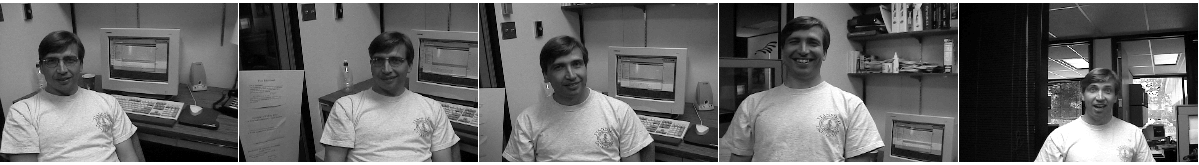
\includegraphics[width=1.0\textwidth]{figs/seq_1_Dudek.png}
								\caption{Dudek dataset.}
								\label{fig:seq_1_Dudek}
								\end{figure}



\begin{table}[h]
\centering
\begin{tabular}{|l|c|c|c|c|}
\hline
&\textbf{maxQ}&\textbf{RofE}&\textbf{nulE}&\textbf{monR}\\\hline
\textbf{2}&-1.00&6.68&7.96&7.85\\\hline
\textbf{4}&8.40&8.19&7.22&8.89\\\hline
\textbf{8}&9.13&7.95&8.67&8.47\\\hline
\textbf{12}&8.34&10.02&8.18&7.60\\\hline
\textbf{16}&8.05&10.08&8.10&9.25\\\hline
\end{tabular}

\caption{Tracking errors for various RVQ configurations.  -1 means that track was lost.  These results show that RVQ is able to track the object of interest very closely.}
\end{table}

For the interested reader, detailed graphical results follow for 8x4 RVQ.
%------------------------------------
\clearpage
\newpage
\subsection{Tracking error}
%------------------------------------

								\begin{figure}[h!]
								\centering
								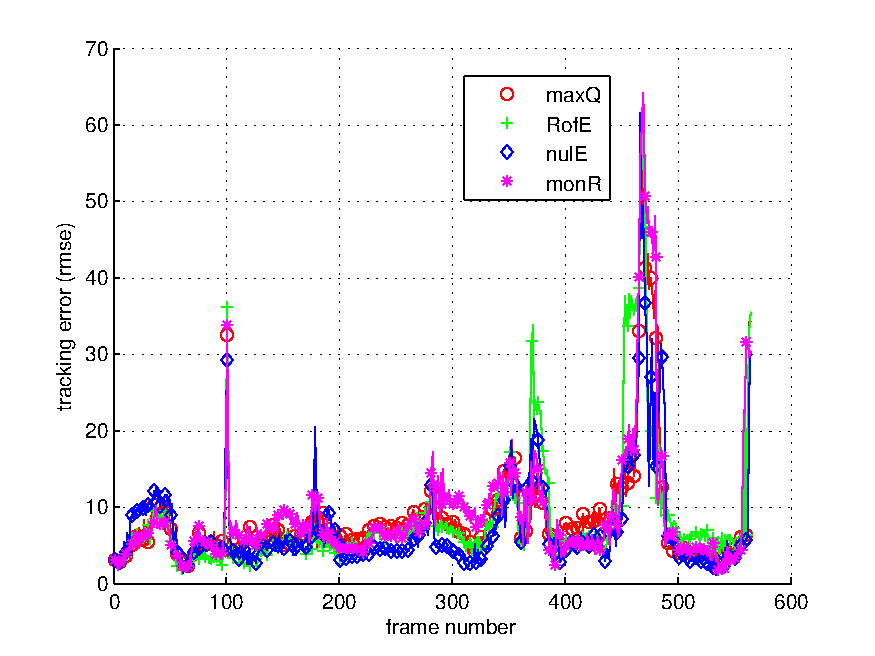
\includegraphics[height=0.38\textheight]{figs/1_Dudek_8_4_1000_trk_rmse.pdf}
								\caption{8x4 RVQ, tracking error (rmse).}
								\label{fig:1_Dudek_8_4_1000_trk_rmse}
								\end{figure}


								\begin{figure}[h!]
								\centering
								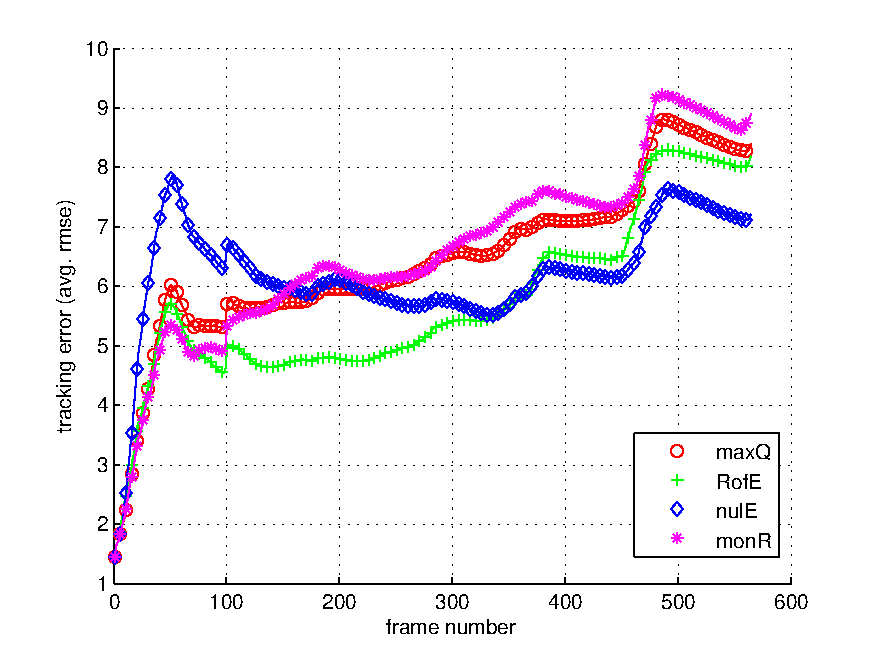
\includegraphics[height=0.38\textheight]{figs/1_Dudek_8_4_1000_trk_armse.pdf}
								\caption{8x4 RVQ, tracking error (average rmse).}
								\label{fig:1_Dudek_8_4_1000_trk_avg_rmse}
								\end{figure}

%------------------------------------
\clearpage
\newpage
\subsection{Target reconstruction}
%------------------------------------

								\begin{figure}[h!]
								\centering
								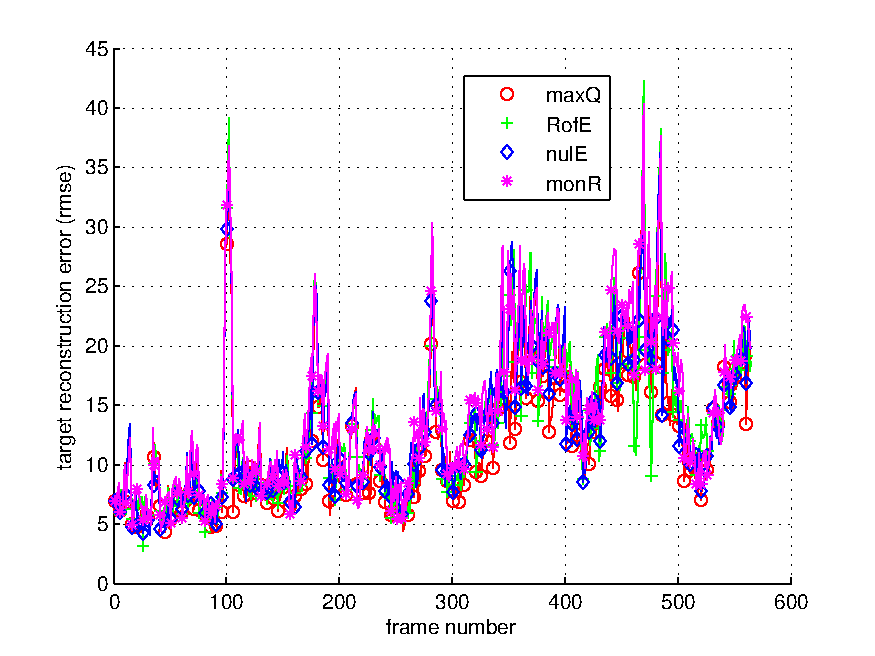
\includegraphics[height=0.4\textheight]{figs/1_Dudek_8_4_1000_snp_rmse.pdf}
								\caption{8x4 RVQ, snippet reconstruction error (rmse).}
								\label{fig:1_Dudek_8_4_1000_snp_rmse}
								\end{figure}


								\begin{figure}[h!]
								\centering
								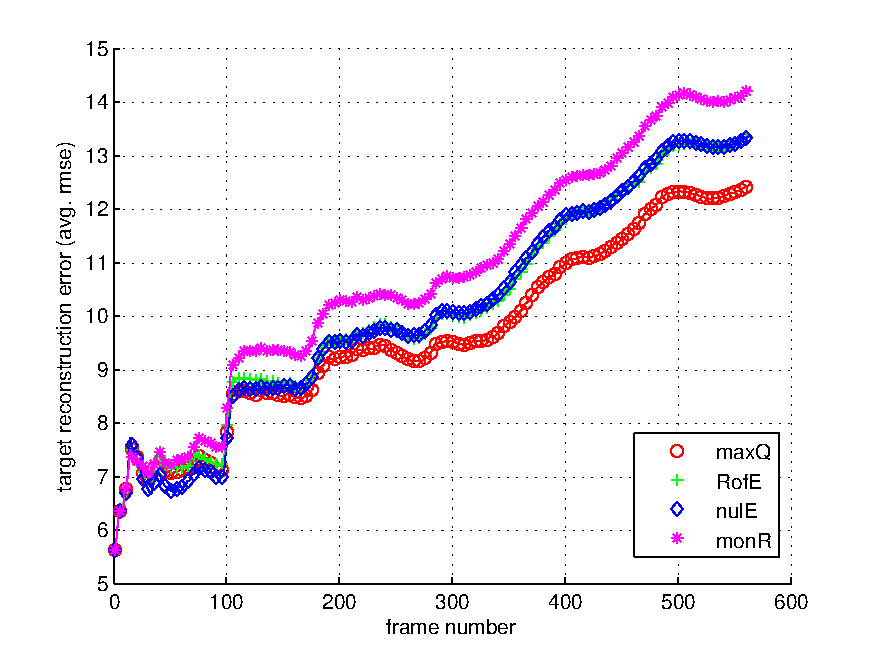
\includegraphics[height=0.4\textheight]{figs/1_Dudek_8_4_1000_snp_armse.pdf}
								\caption{8x4 RVQ, snippet reconstruction error (avg. rmse).}
								\label{fig:1_Dudek_8_4_1000_snp_armse}
								\end{figure}

								\begin{figure}[h!]
								\centering
								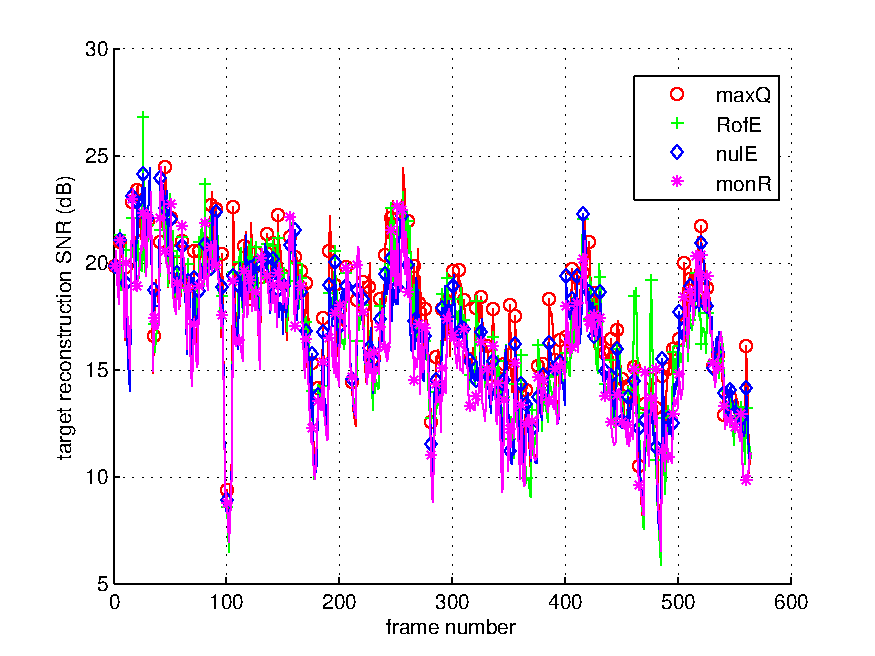
\includegraphics[height=0.4\textheight]{figs/1_Dudek_8_4_1000_snp_SNRdB.pdf}
								\caption{8x4 RVQ, snippet reconstruction SNR in dB.}
								\label{fig:1_Dudek_8_4_1000_snp_SNRdB}
								\end{figure}
%------------------------------------
\clearpage
\newpage
\subsection{Learning}
%------------------------------------
								\begin{figure}[h!]
								\centering
								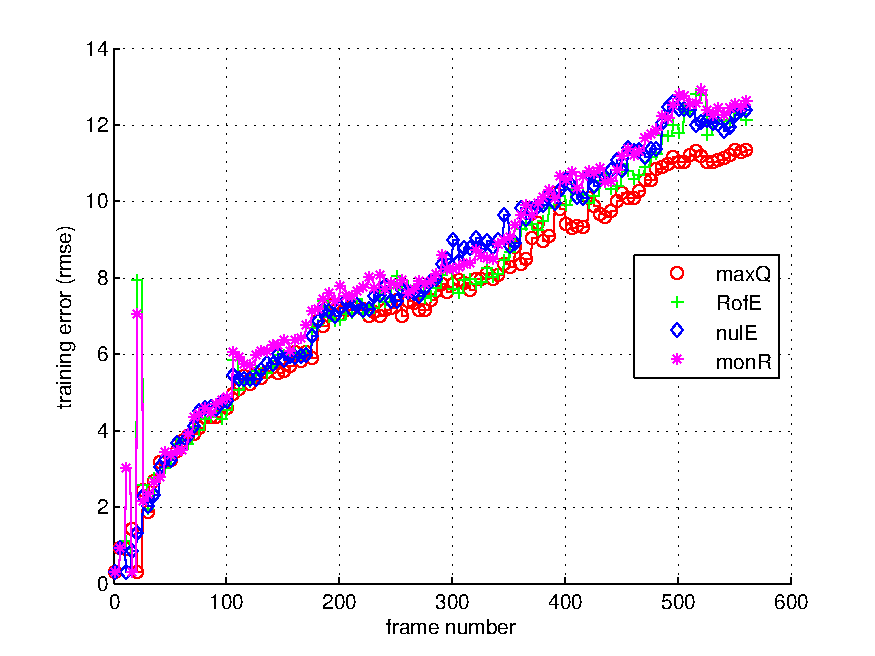
\includegraphics[height=0.4\textheight]{figs/1_Dudek_8_4_1000_trg_rmse.pdf}
								\caption{8x4 RVQ, training error (rmse).}
								\label{fig:1_Dudek_8_4_1000_trg_rmse}
								\end{figure}


								\begin{figure}[h!]
								\centering
								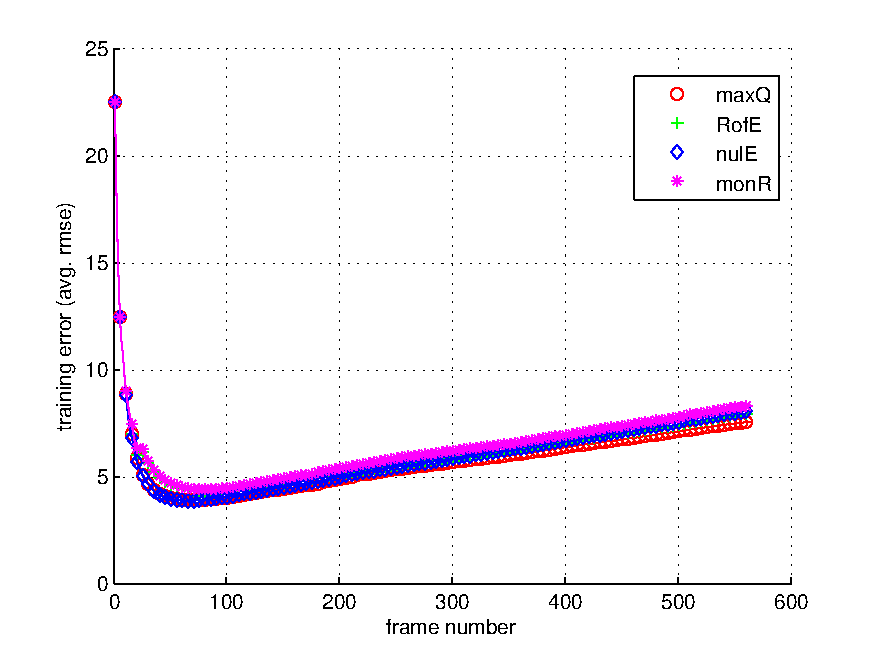
\includegraphics[height=0.4\textheight]{figs/1_Dudek_8_4_1000_trg_armse.pdf}
								\caption{8x4 RVQ, training error (avg. rmse).}
								\label{fig:1_Dudek_8_4_1000_trg_armse}
								\end{figure}

								\begin{figure}[h!]
								\centering
								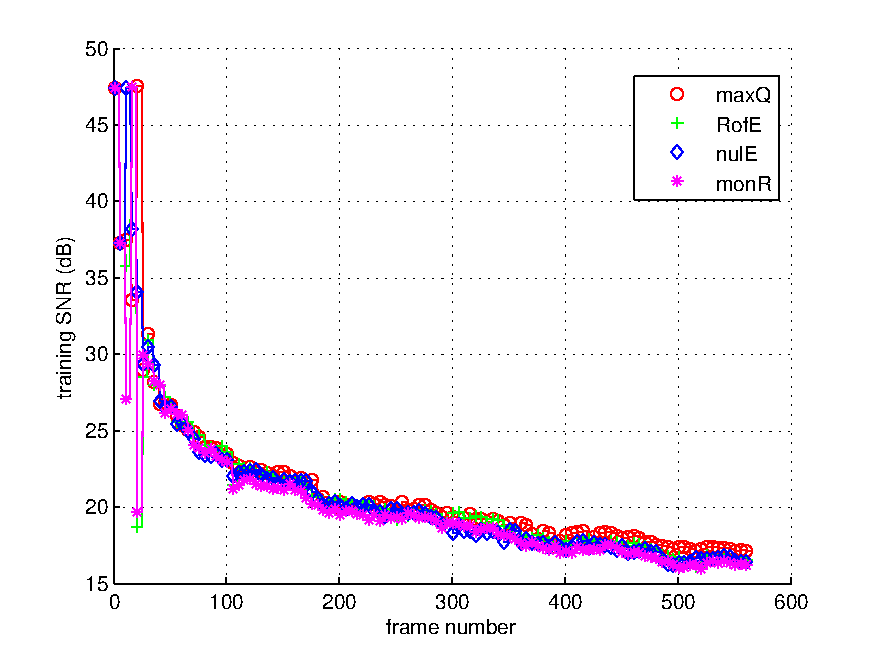
\includegraphics[height=0.4\textheight]{figs/1_Dudek_8_4_1000_trg_SNRdB.pdf}
								\caption{8x4 RVQ, training SNR in dB.}
								\label{fig:1_Dudek_8_4_1000_trg_SNRdB}
								\end{figure}
%------------------------------------
\clearpage
\newpage
\subsection{Testing}
%------------------------------------
								\begin{figure}[h!]
								\centering
								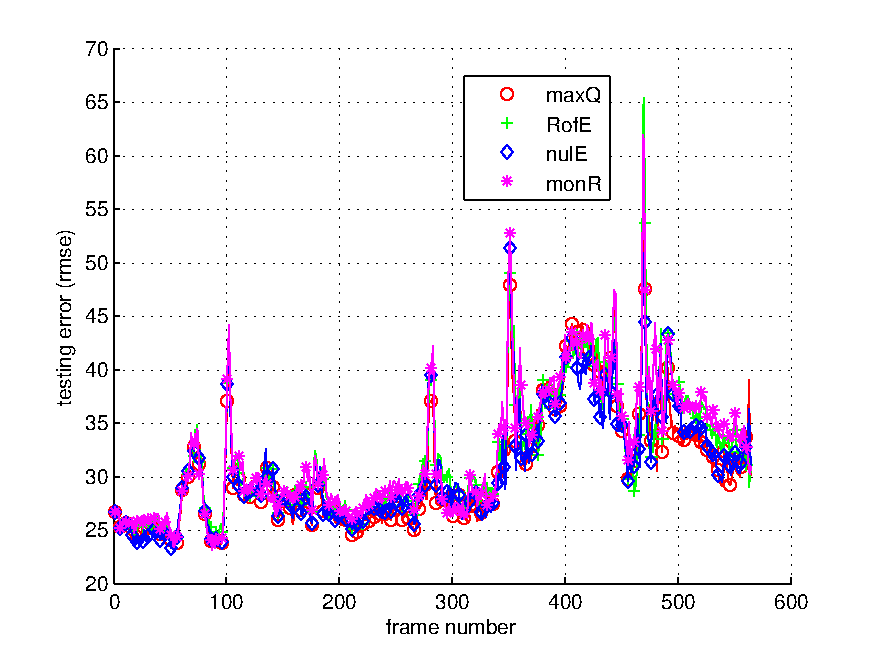
\includegraphics[height=0.4\textheight]{figs/1_Dudek_8_4_1000_tst_rmse.pdf}
								\caption{8x4 RVQ, testing error (rmse).}
								\label{fig:1_Dudek_8_4_1000_tst_rmse}
								\end{figure}


								\begin{figure}[h!]
								\centering
								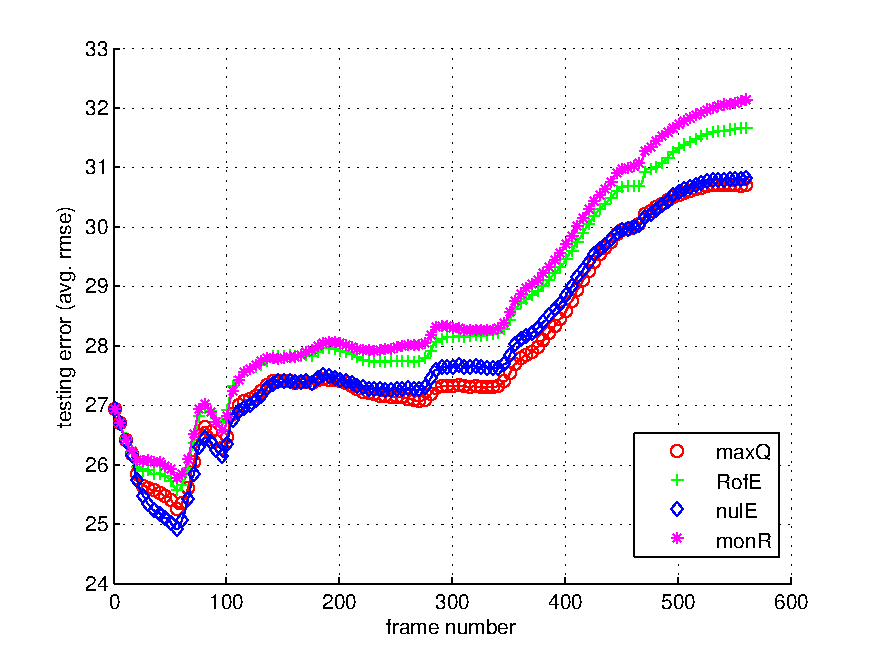
\includegraphics[height=0.4\textheight]{figs/1_Dudek_8_4_1000_tst_armse.pdf}
								\caption{8x4 RVQ, testing error (avg. rmse).}
								\label{fig:1_Dudek_8_4_1000_tst_armse}
								\end{figure}

								\begin{figure}[h!]
								\centering
								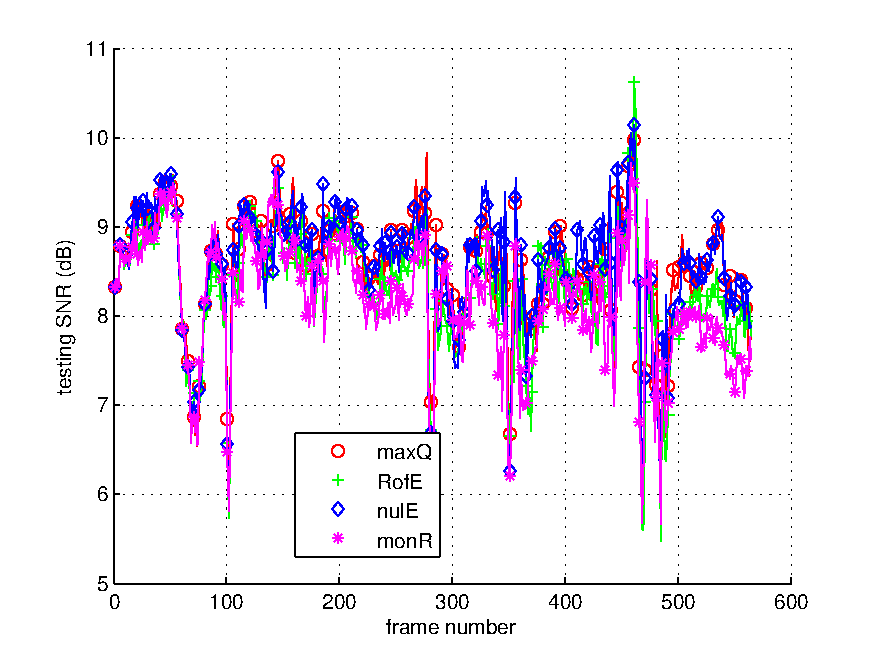
\includegraphics[height=0.4\textheight]{figs/1_Dudek_8_4_1000_tst_SNRdB.pdf}
								\caption{8x4 RVQ,testing SNR in dB.}
								\label{fig:1_Dudek_8_4_1000_tst_SNRdB}
								\end{figure}
%%===============================
\clearpage
\newpage
\section{Tracking: David dataset} 
%===============================
								\begin{figure}[h!]
								\centering
								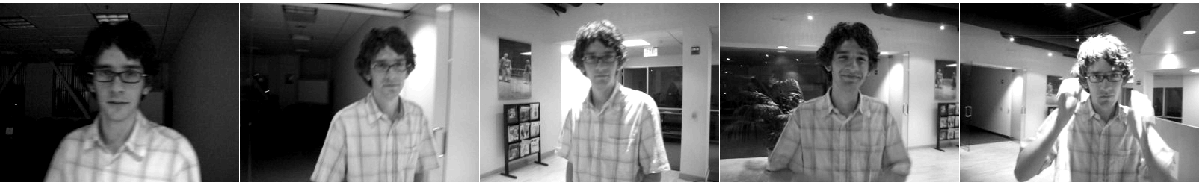
\includegraphics[width=1.0\textwidth]{figs/seq_2_davidin300.png}
								\caption{David dataset.}
								\label{fig:seq_1_David}
								\end{figure}



\begin{table}[h]
\centering
\begin{tabular}{|l|c|c|c|c|}
\hline
&\textbf{maxQ}&\textbf{RofE}&\textbf{nulE}&\textbf{monR}\\\hline
\textbf{2}&5.67&6.93&8.72&11.31\\\hline
\textbf{4}&4.39&5.95&4.59&5.00\\\hline
\textbf{8}&8.08&6.14&8.50&8.52\\\hline
\textbf{12}&6.07&5.65&6.70&4.52\\\hline
\textbf{16}&5.48&5.33&4.60&4.29\\\hline
\end{tabular}

\caption{Tracking errors for various RVQ configurations.  -1 means that track was lost.  These results show that RVQ is able to track the object of interest very closely.}
\end{table}

For the interested reader, detailed graphical results follow for 8x4 RVQ.

%------------------------------------
\clearpage
\newpage
\subsection{Tracking error}
%------------------------------------

								\begin{figure}[h!]
								\centering
								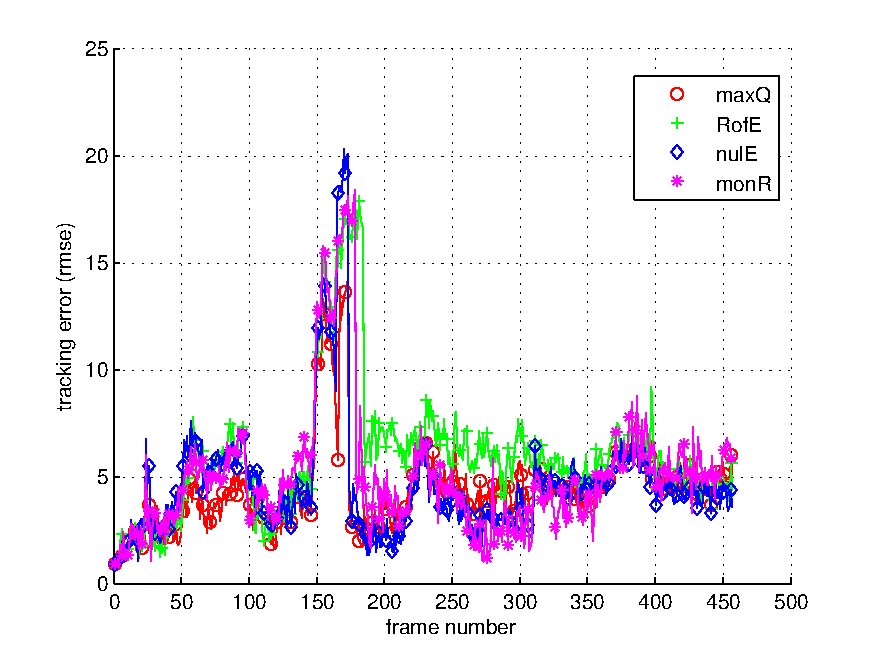
\includegraphics[height=0.38\textheight]{figs/2_davidin300_8_4_1000_trk_rmse.pdf}
								\caption{8x4 RVQ, tracking error (rmse).}
								\label{fig:2_davidin300_8_4_1000_trk_rmse}
								\end{figure}


								\begin{figure}[h!]
								\centering
								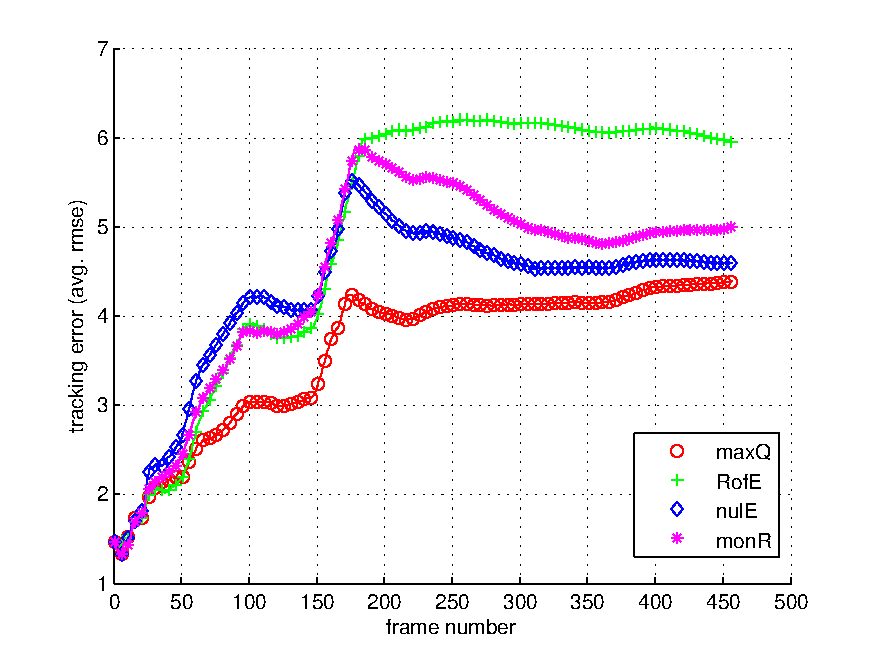
\includegraphics[height=0.38\textheight]{figs/2_davidin300_8_4_1000_trk_armse.pdf}
								\caption{8x4 RVQ, tracking error (average rmse).}
								\label{fig:2_davidin300_8_4_1000_trk_avg_rmse}
								\end{figure}

%------------------------------------
\clearpage
\newpage
\subsection{Target reconstruction}
%------------------------------------

								\begin{figure}[h!]
								\centering
								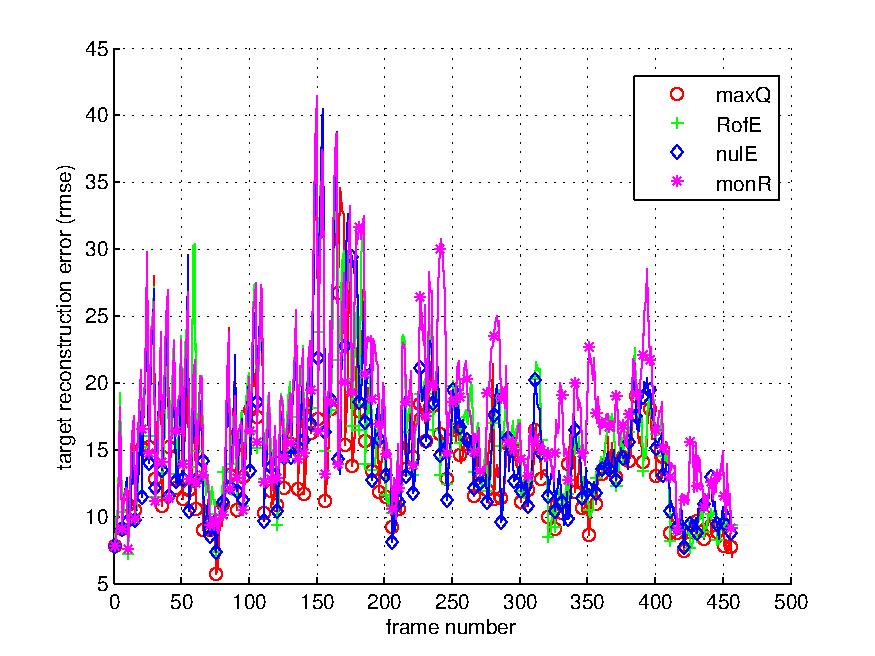
\includegraphics[height=0.4\textheight]{figs/2_davidin300_8_4_1000_snp_rmse.pdf}
								\caption{8x4 RVQ, snippet reconstruction error (rmse).}
								\label{fig:2_davidin300_8_4_1000_snp_rmse}
								\end{figure}


								\begin{figure}[h!]
								\centering
								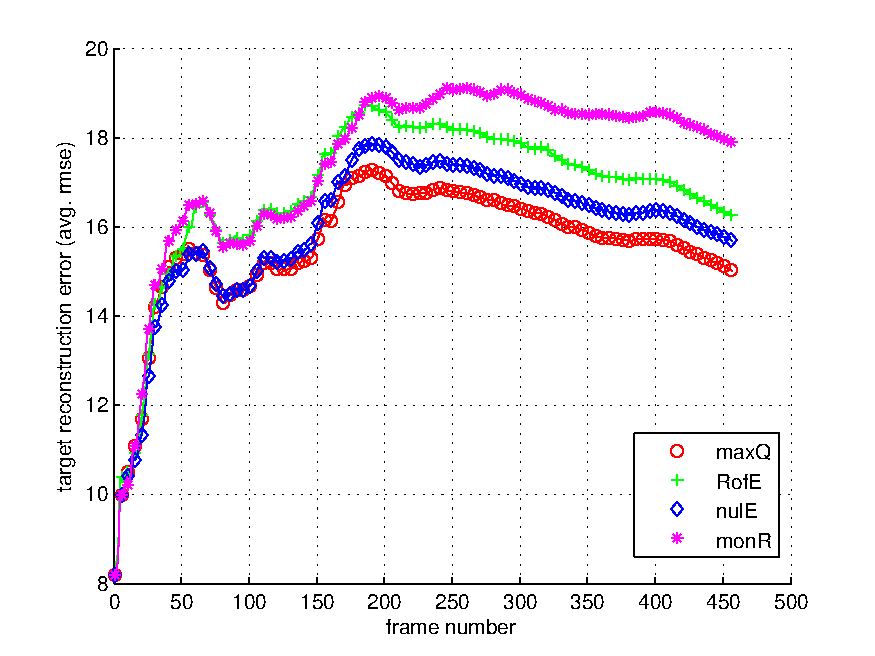
\includegraphics[height=0.4\textheight]{figs/2_davidin300_8_4_1000_snp_armse.pdf}
								\caption{8x4 RVQ, snippet reconstruction error (avg. rmse).}
								\label{fig:2_davidin300_8_4_1000_snp_armse}
								\end{figure}

								\begin{figure}[h!]
								\centering
								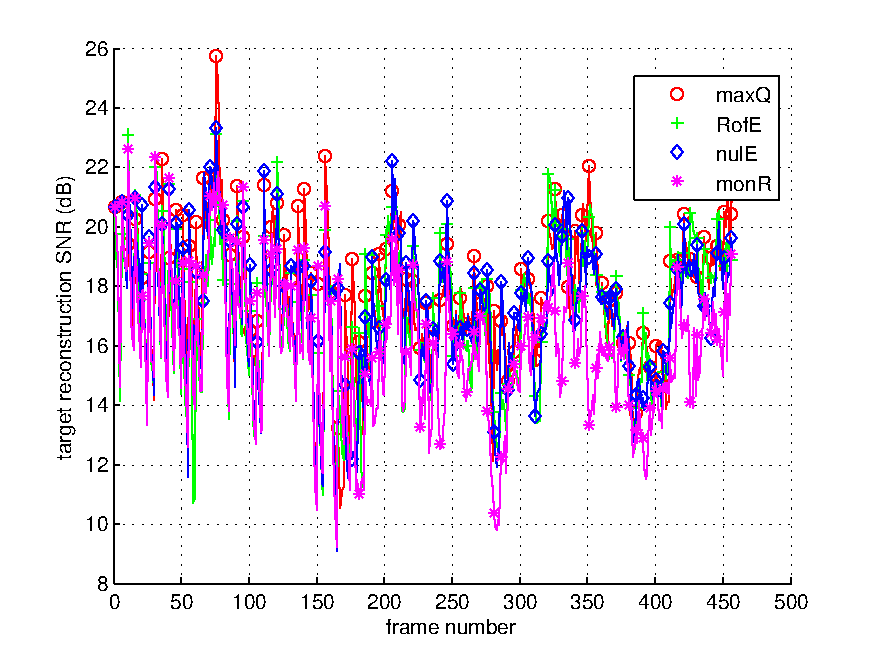
\includegraphics[height=0.4\textheight]{figs/2_davidin300_8_4_1000_snp_SNRdB.pdf}
								\caption{8x4 RVQ, snippet reconstruction SNR in dB.}
								\label{fig:2_davidin300_8_4_1000_snp_SNRdB}
								\end{figure}
%------------------------------------
\clearpage
\newpage
\subsection{Learning}
%------------------------------------

								\begin{figure}[h!]
								\centering
								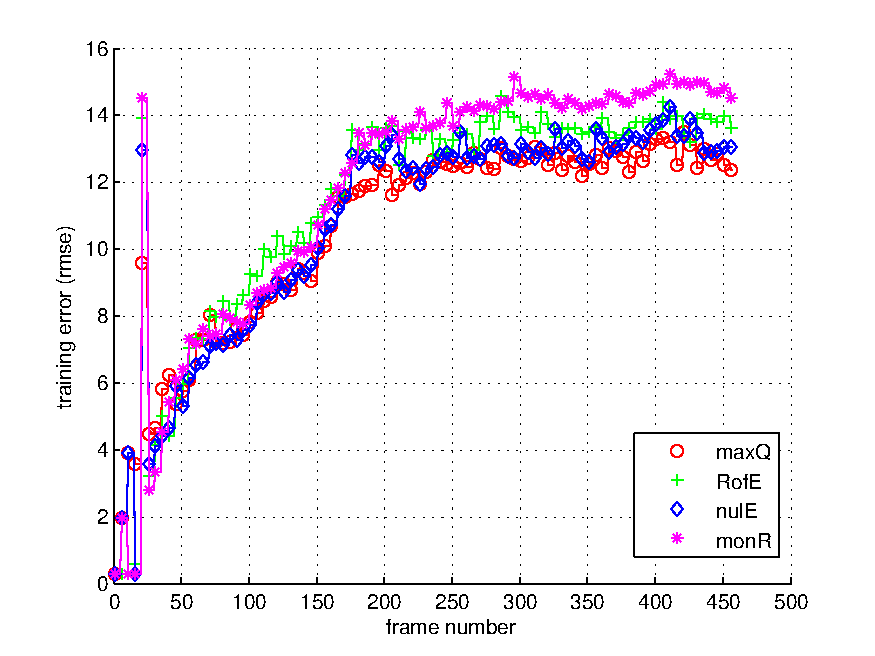
\includegraphics[height=0.4\textheight]{figs/2_davidin300_8_4_1000_trg_rmse.pdf}
								\caption{8x4 RVQ, training error (rmse).}
								\label{fig:2_davidin300_8_4_1000_trg_rmse}
								\end{figure}


								\begin{figure}[h!]
								\centering
								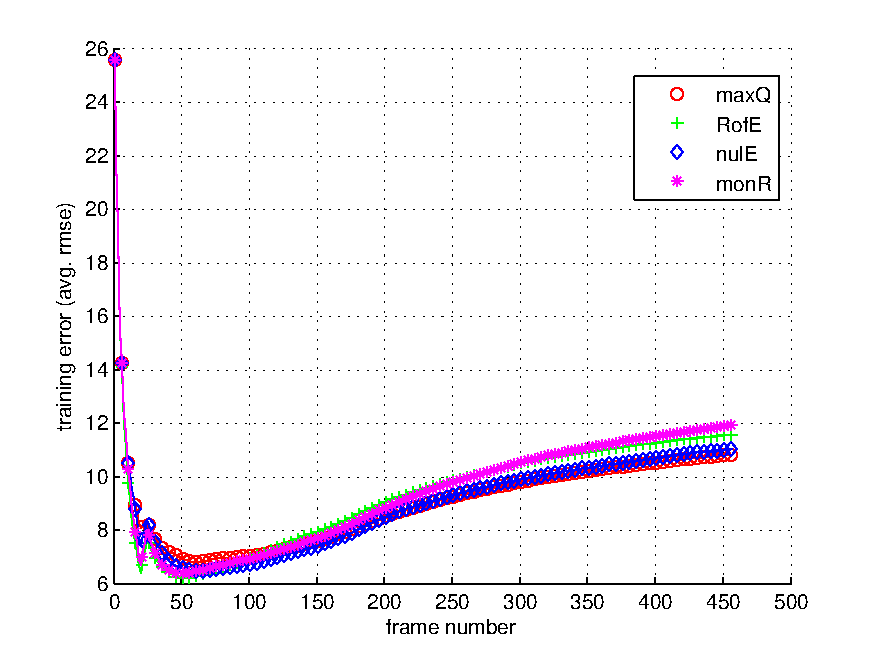
\includegraphics[height=0.4\textheight]{figs/2_davidin300_8_4_1000_trg_armse.pdf}
								\caption{8x4 RVQ, training error (avg. rmse).}
								\label{fig:2_davidin300_8_4_1000_trg_armse}
								\end{figure}

								\begin{figure}[h!]
								\centering
								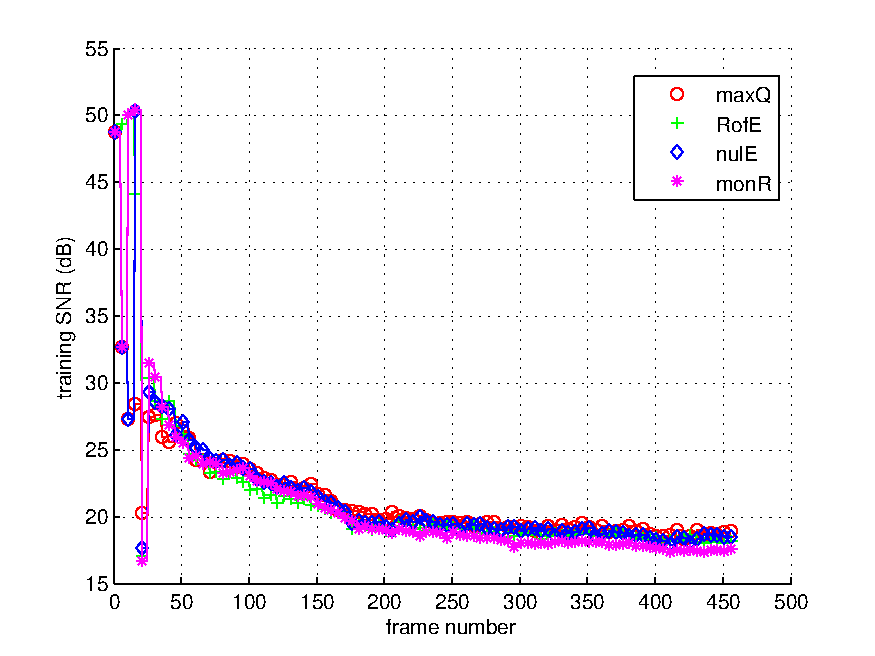
\includegraphics[height=0.4\textheight]{figs/2_davidin300_8_4_1000_trg_SNRdB.pdf}
								\caption{8x4 RVQ, training SNR in dB.}
								\label{fig:2_davidin300_8_4_1000_trg_SNRdB}
								\end{figure}
%------------------------------------
\clearpage
\newpage
\subsection{Testing}
%------------------------------------
								\begin{figure}[h!]
								\centering
								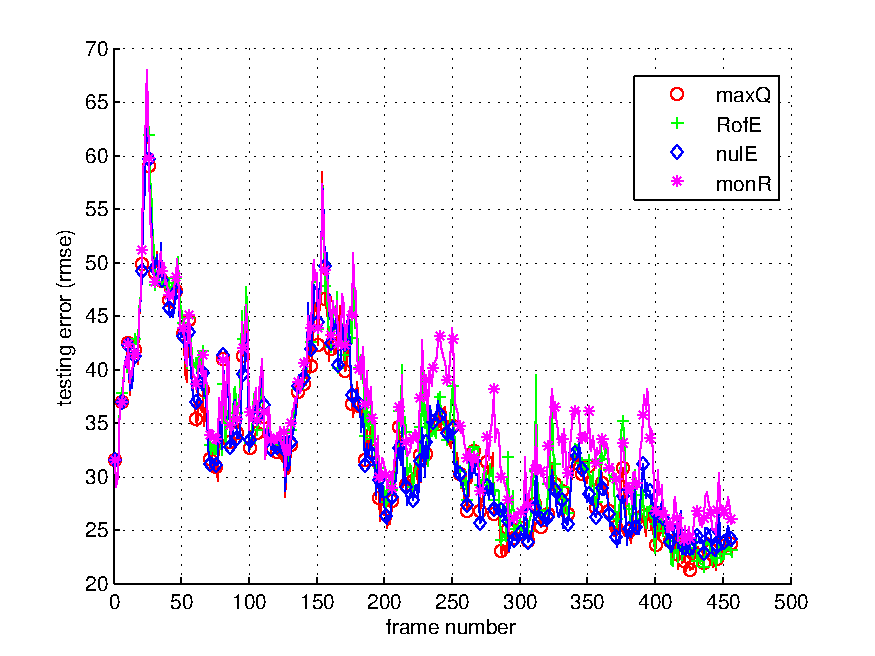
\includegraphics[height=0.4\textheight]{figs/2_davidin300_8_4_1000_tst_rmse.pdf}
								\caption{8x4 RVQ, testing error (rmse).}
								\label{fig:2_davidin300_8_4_1000_tst_rmse}
								\end{figure}


								\begin{figure}[h!]
								\centering
								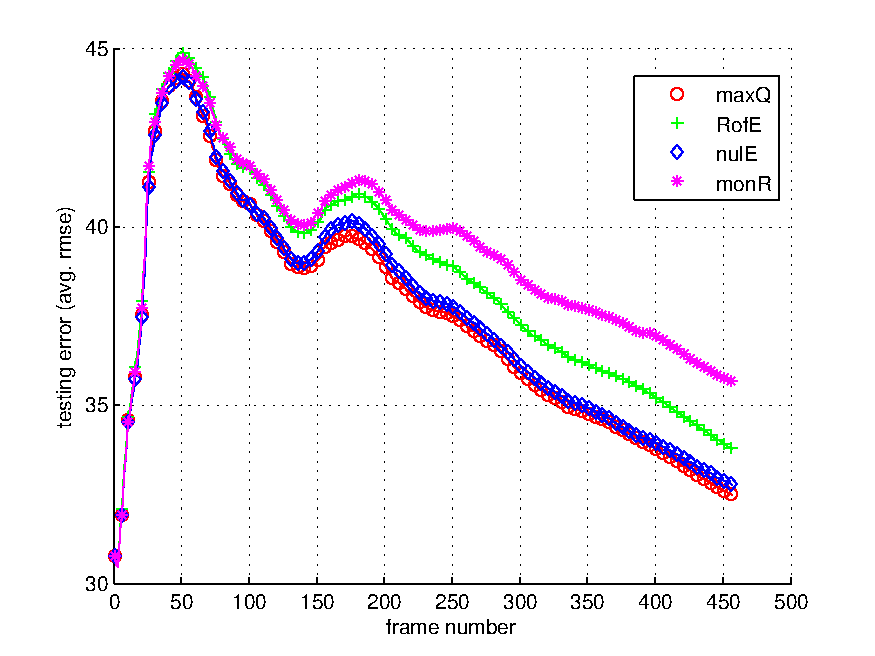
\includegraphics[height=0.4\textheight]{figs/2_davidin300_8_4_1000_tst_armse.pdf}
								\caption{8x4 RVQ, testing error (avg. rmse).}
								\label{fig:2_davidin300_8_4_1000_tst_armse}
								\end{figure}

								\begin{figure}[h!]
								\centering
								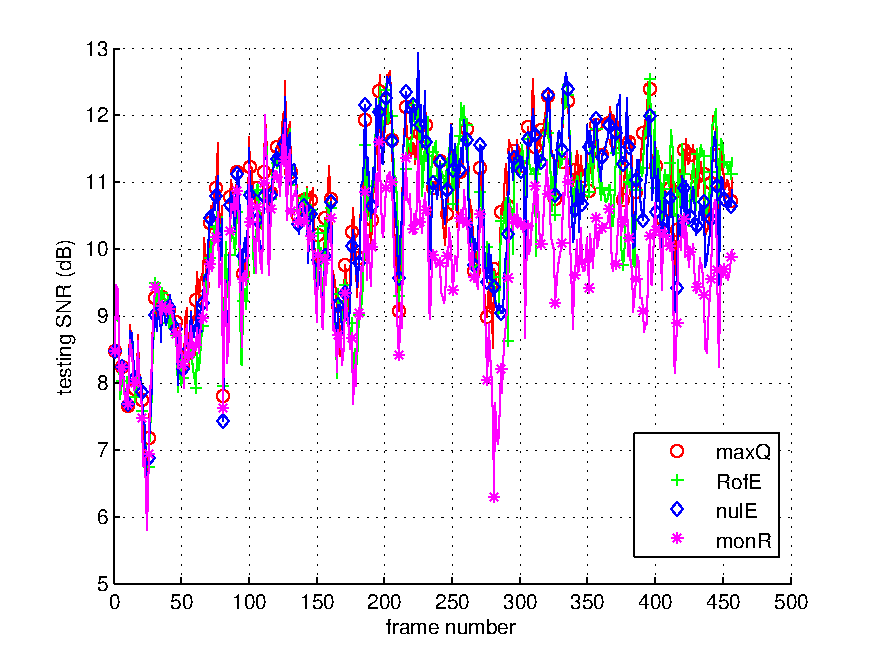
\includegraphics[height=0.4\textheight]{figs/2_davidin300_8_4_1000_tst_SNRdB.pdf}
								\caption{8x4 RVQ,testing SNR in dB.}
								\label{fig:2_davidin300_8_4_1000_tst_SNRdB}
								\end{figure}

%%===============================
\clearpage
\newpage
\section{Tracking: sylv dataset} 
%===============================
								\begin{figure}[h!]
								\centering
								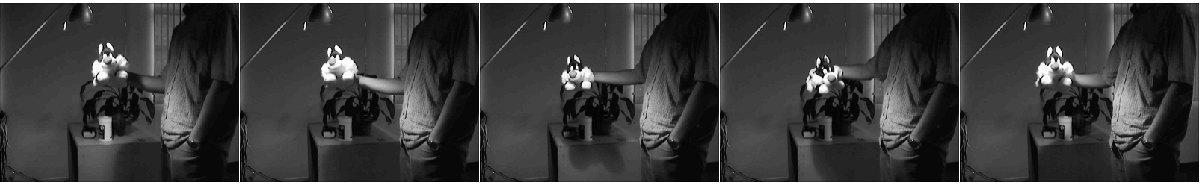
\includegraphics[width=1.0\textwidth]{figs/seq_3_sylv.png}
								\caption{sylv dataset.}
								\label{fig:seq_3_sylv}
								\end{figure}



\begin{table}[h]
\centering
\begin{tabular}{|l|c|c|c|c|}
\hline
&\textbf{maxQ}&\textbf{RofE}&\textbf{nulE}&\textbf{monR}\\\hline
\textbf{2}&4.26&4.29&4.72&5.61\\\hline
\textbf{4}&4.69&4.66&4.82&4.70\\\hline
\textbf{8}&4.66&4.56&4.88&4.95\\\hline
\textbf{12}&4.19&5.03&4.43&4.96\\\hline
\textbf{16}&4.89&4.54&4.77&4.69\\\hline
\end{tabular}

\caption{Tracking errors for various RVQ configurations.  -1 means that track was lost.  These results show that RVQ is able to track the object of interest very closely.}
\end{table}

For the interested reader, detailed graphical results follow for 8x4 RVQ.
%------------------------------------
\clearpage
\newpage
\subsection{Tracking error}
%------------------------------------

								\begin{figure}[h!]
								\centering
								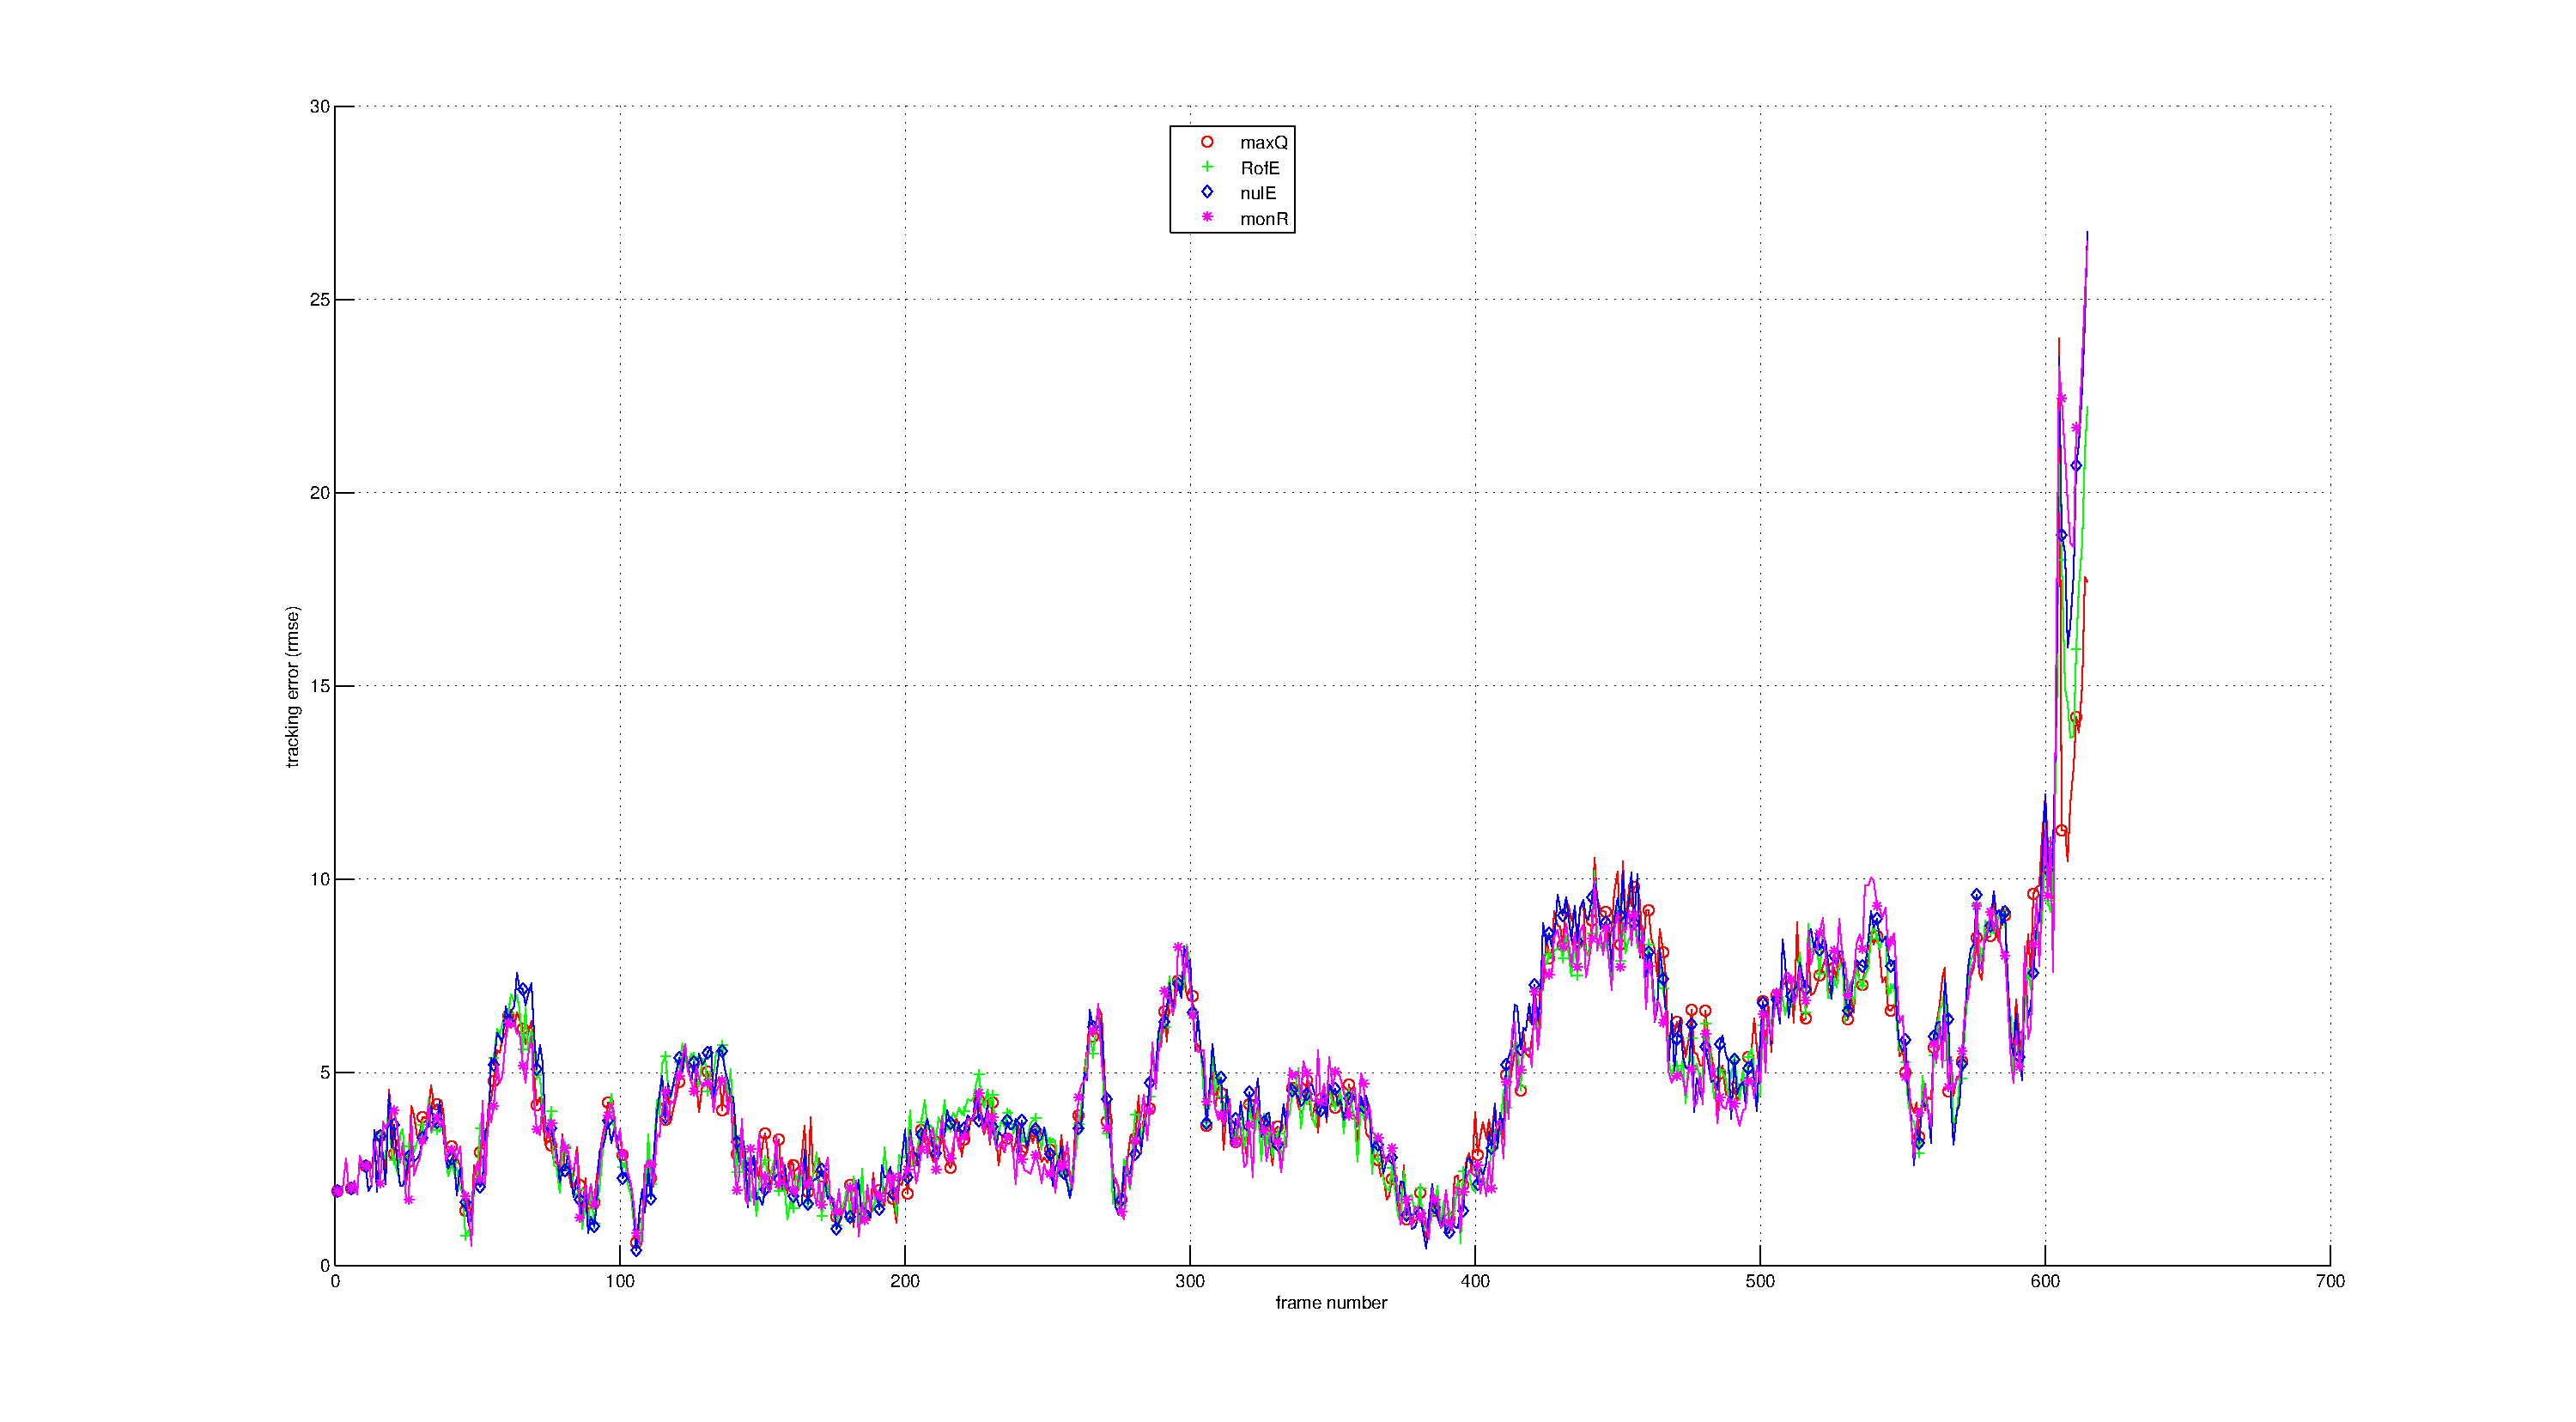
\includegraphics[height=0.38\textheight]{figs/3_sylv_8_4_1000_trk_rmse.pdf}
								\caption{8x4 RVQ, tracking error (rmse).}
								\label{fig:3_sylv_8_4_1000_trk_rmse}
								\end{figure}


								\begin{figure}[h!]
								\centering
								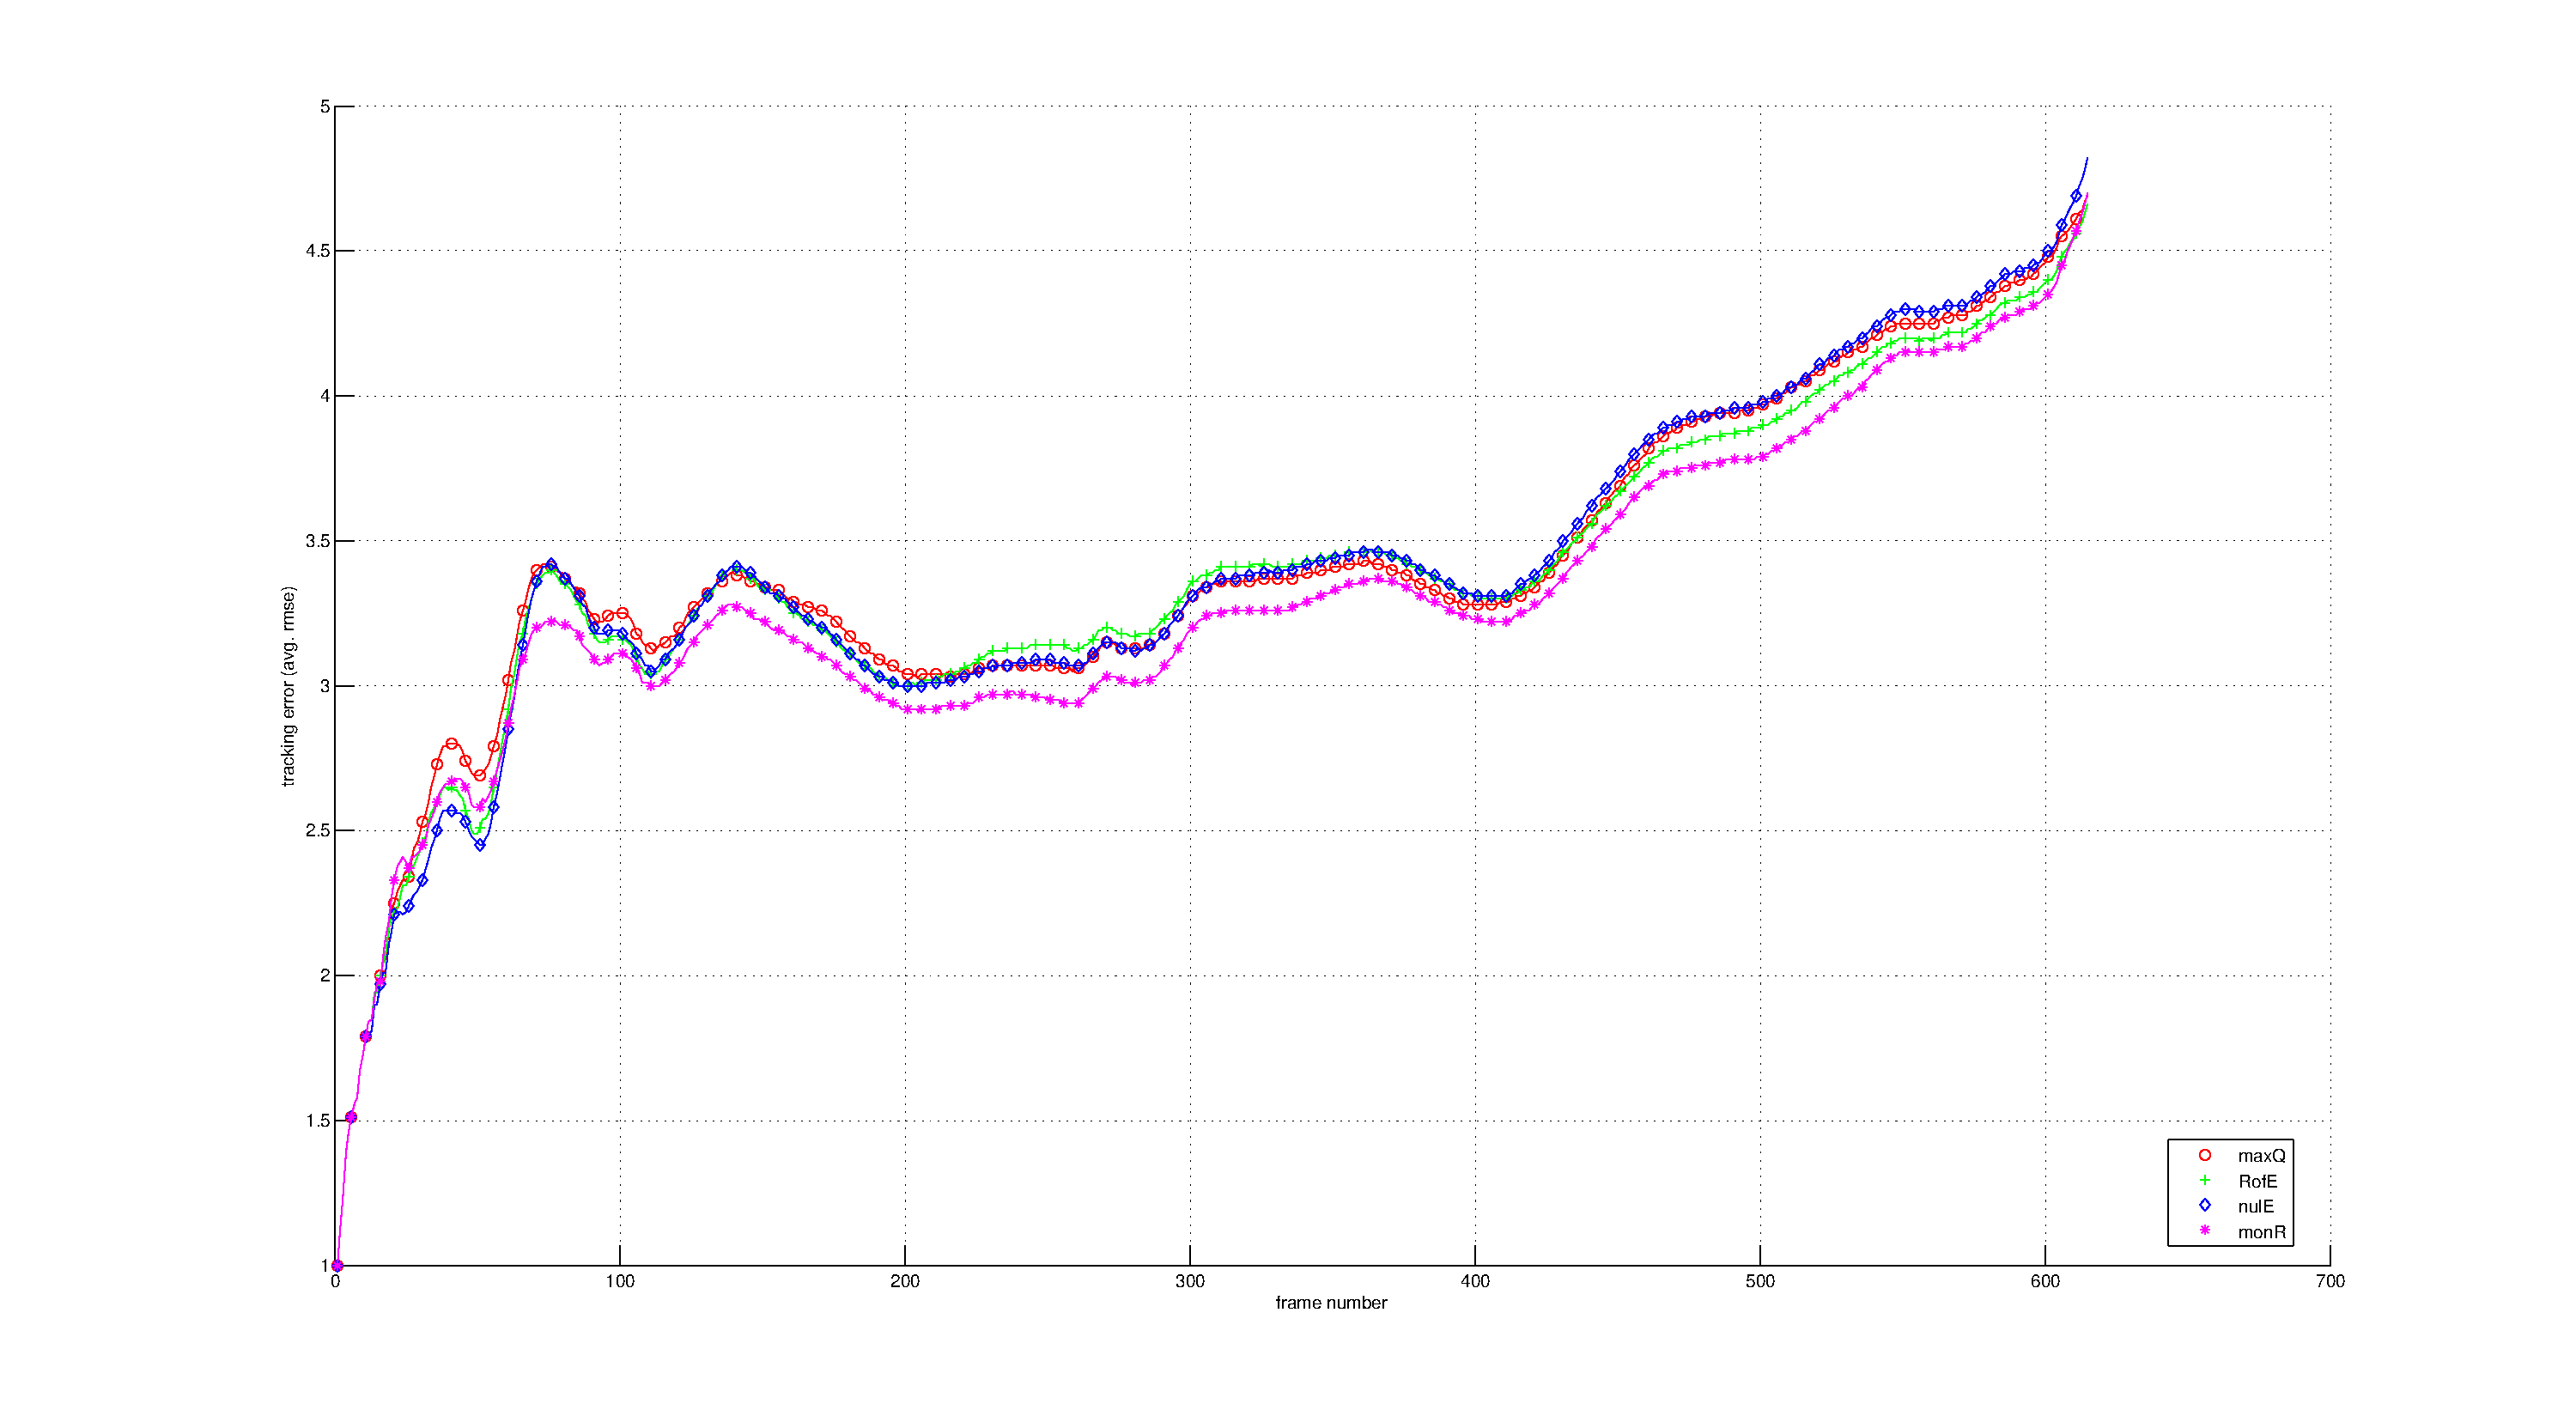
\includegraphics[height=0.38\textheight]{figs/3_sylv_8_4_1000_trk_armse.pdf}
								\caption{8x4 RVQ, tracking error (average rmse).}
								\label{fig:3_sylv_8_4_1000_trk_avg_rmse}
								\end{figure}

%------------------------------------
\clearpage
\newpage
\subsection{Target reconstruction}
%------------------------------------

								\begin{figure}[h!]
								\centering
								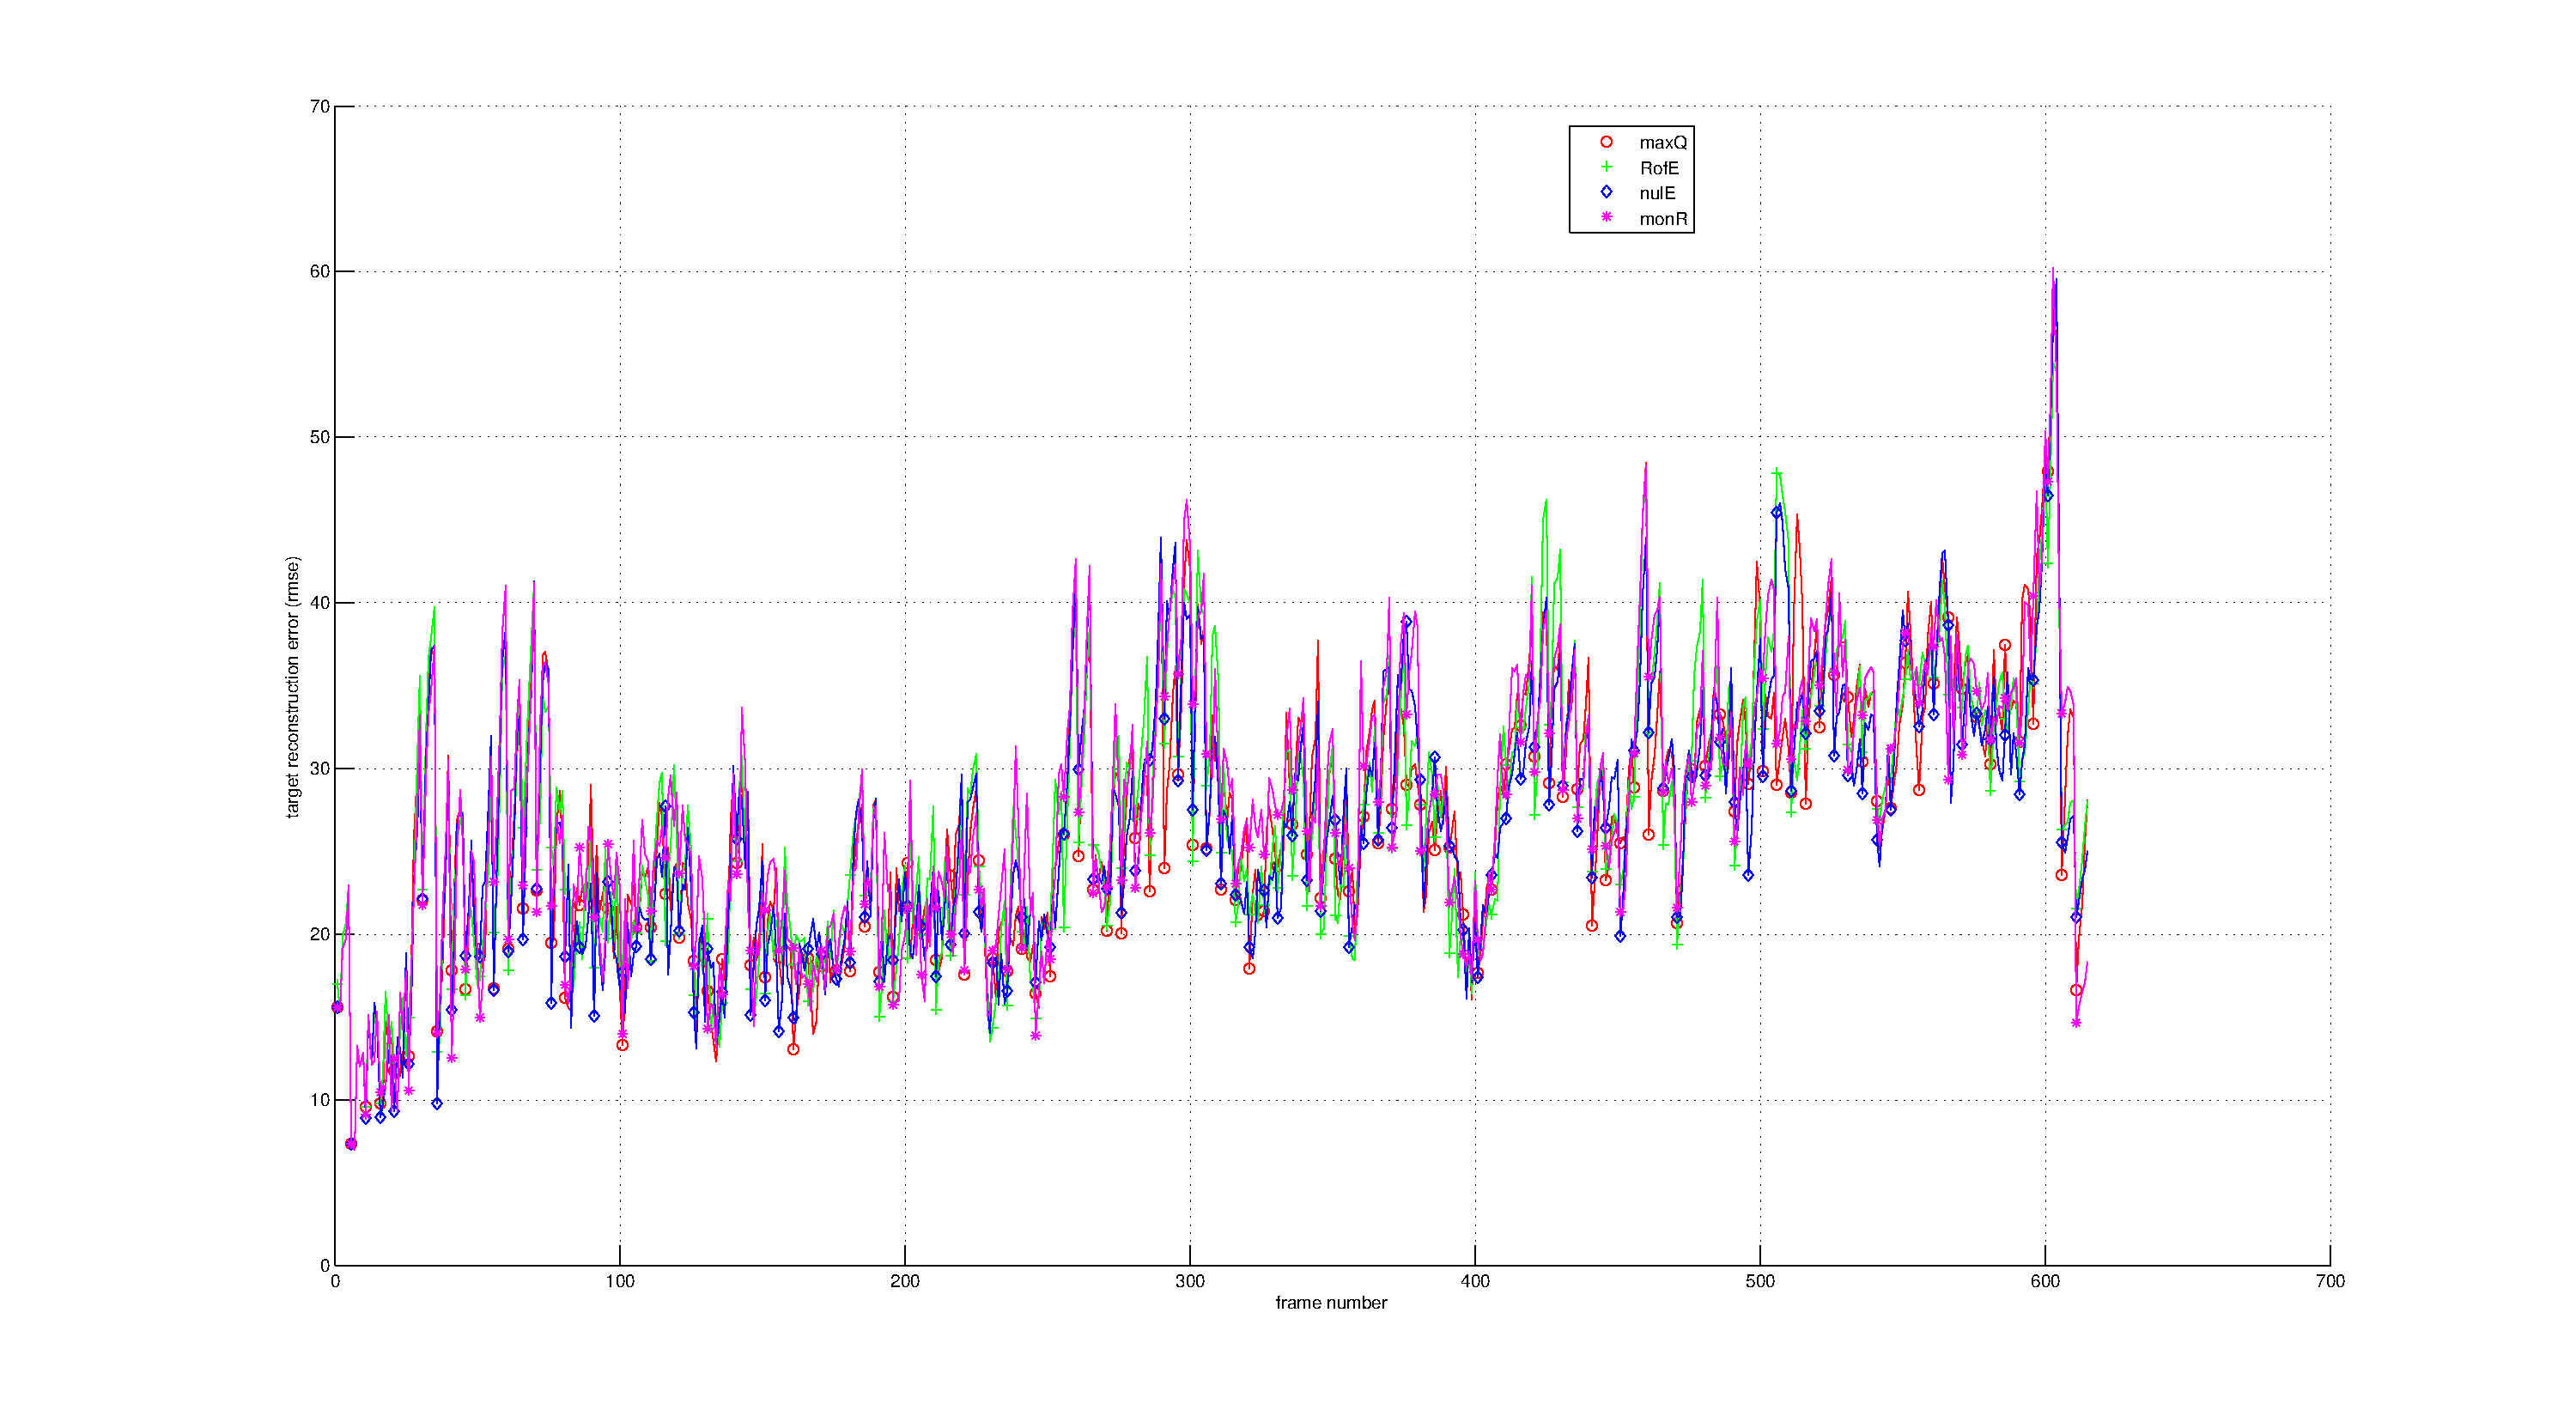
\includegraphics[height=0.4\textheight]{figs/3_sylv_8_4_1000_snp_rmse.pdf}
								\caption{8x4 RVQ, snippet reconstruction error (rmse).}
								\label{fig:3_sylv_8_4_1000_snp_rmse}
								\end{figure}


								\begin{figure}[h!]
								\centering
								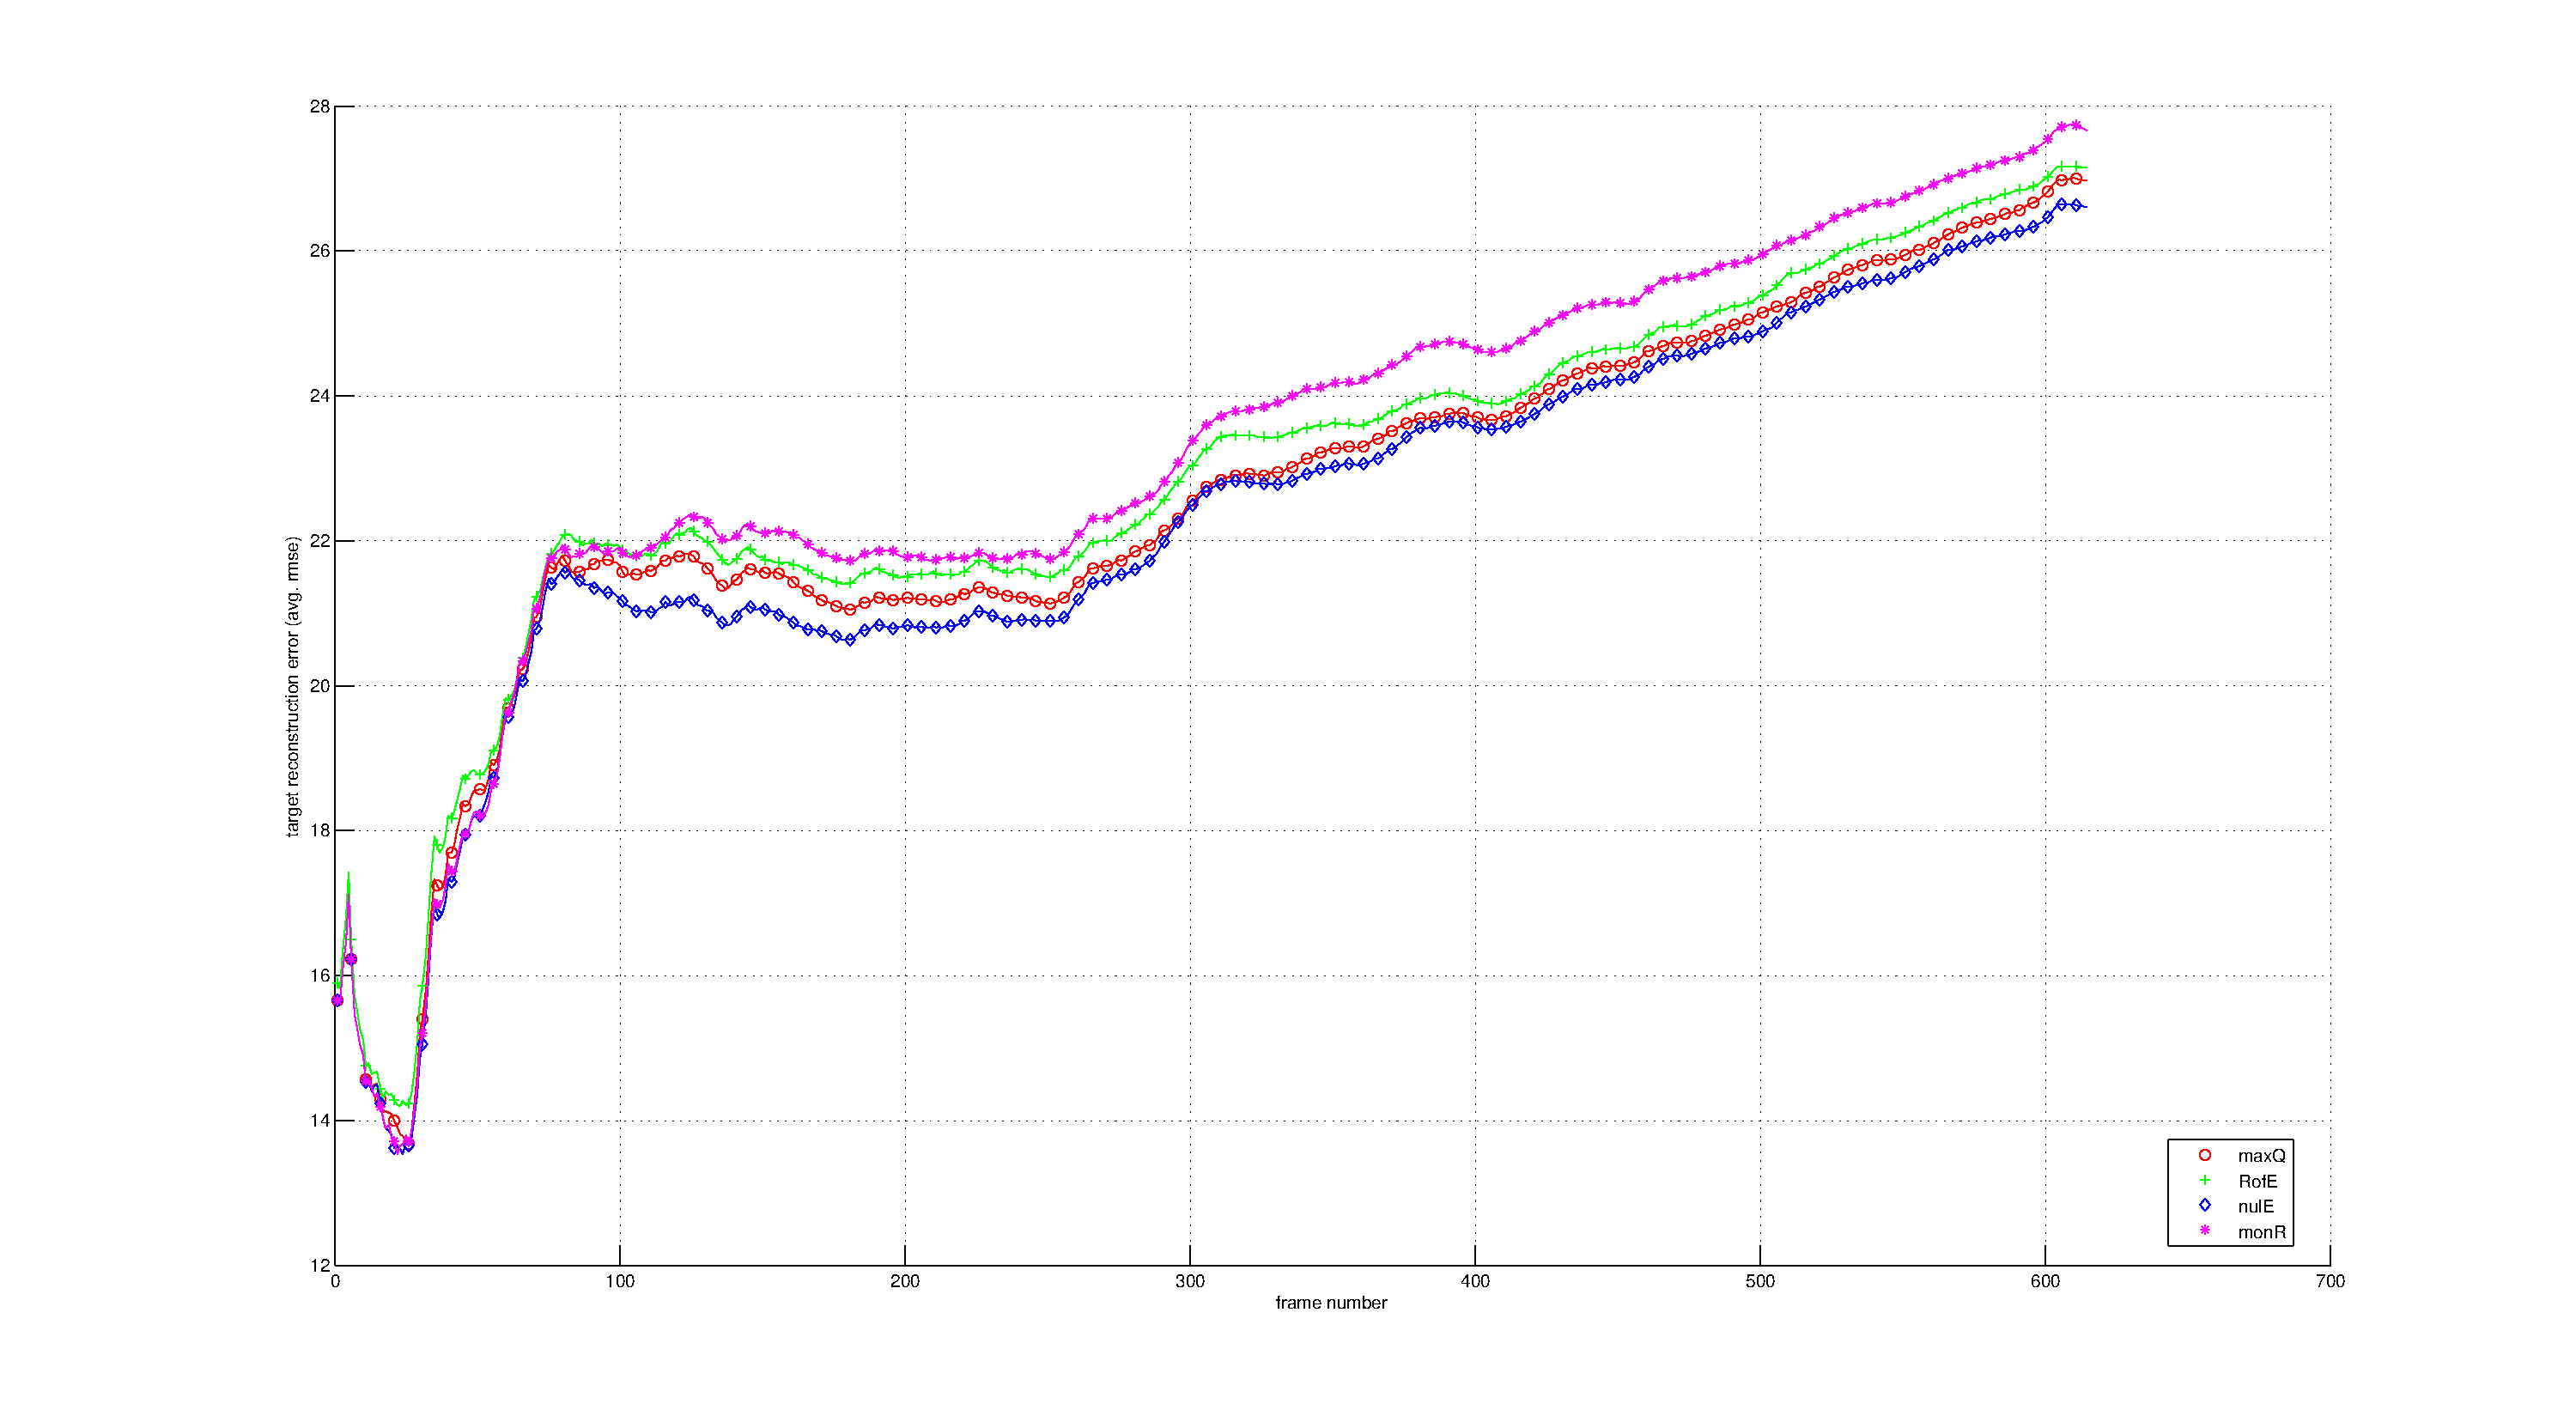
\includegraphics[height=0.4\textheight]{figs/3_sylv_8_4_1000_snp_armse.pdf}
								\caption{8x4 RVQ, snippet reconstruction error (avg. rmse).}
								\label{fig:3_sylv_8_4_1000_snp_armse}
								\end{figure}

								\begin{figure}[h!]
								\centering
								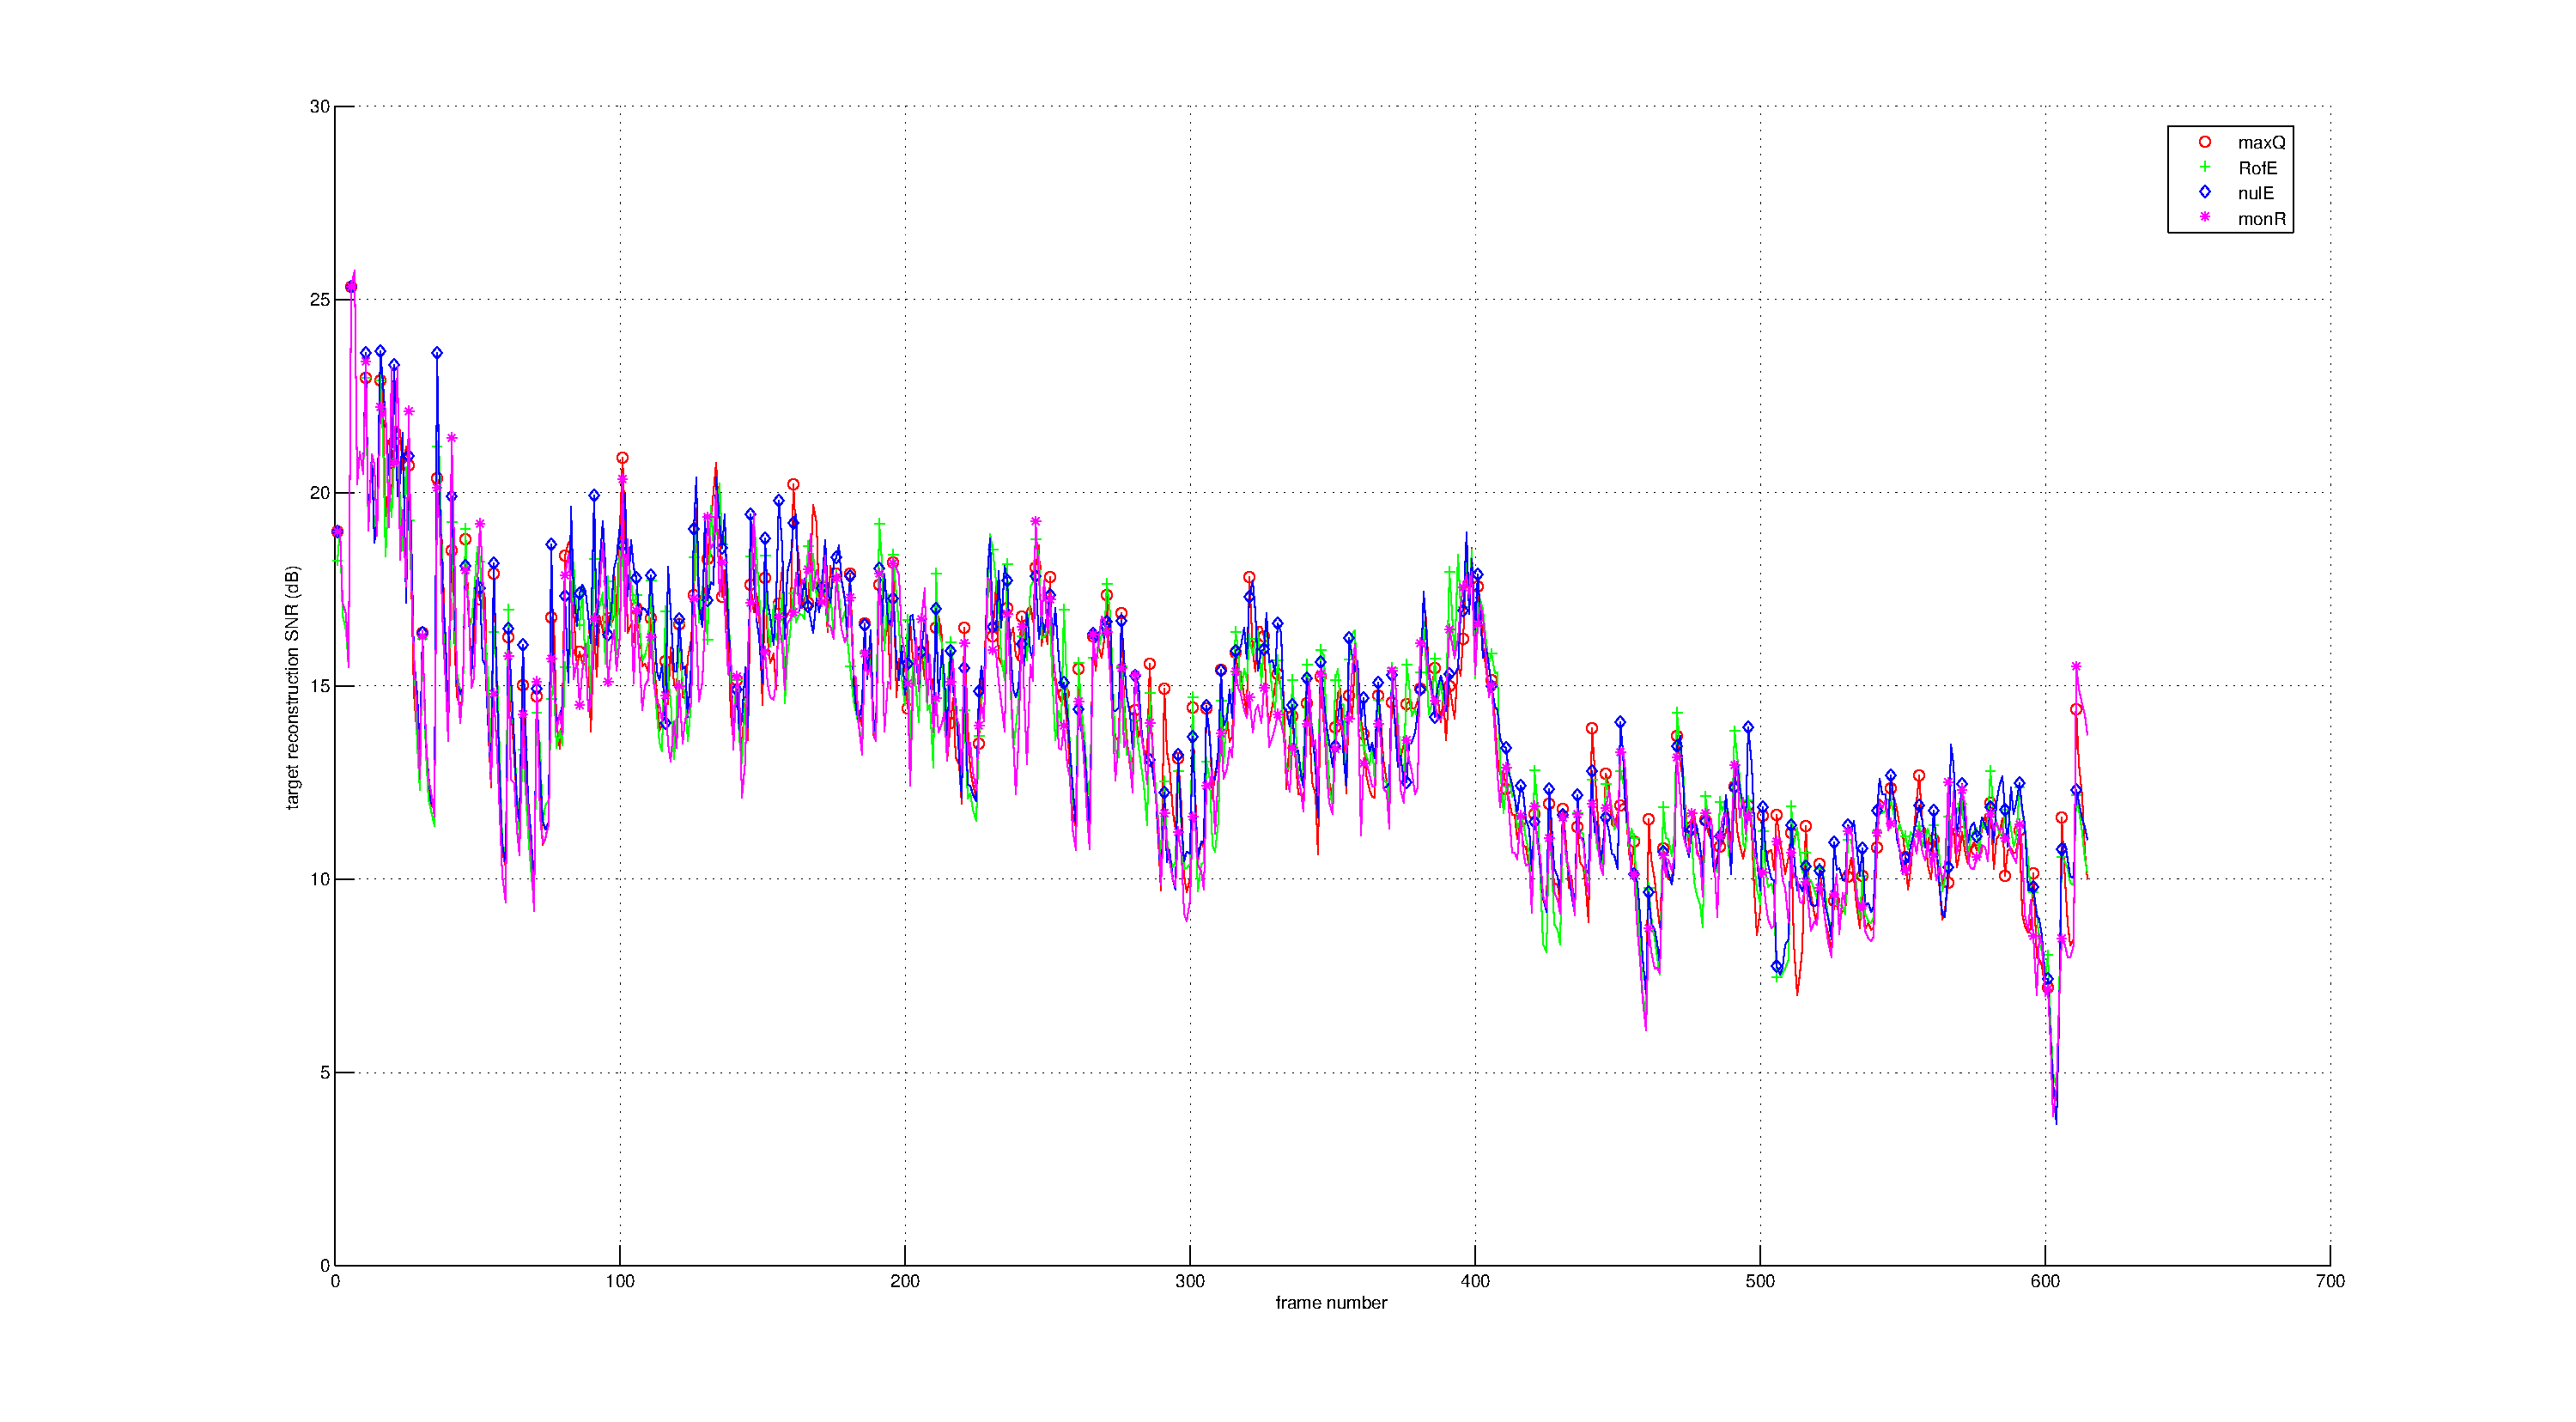
\includegraphics[height=0.4\textheight]{figs/3_sylv_8_4_1000_snp_SNRdB.pdf}
								\caption{8x4 RVQ, snippet reconstruction SNR in dB.}
								\label{fig:3_sylv_8_4_1000_snp_SNRdB}
								\end{figure}
%------------------------------------
\clearpage
\newpage
\subsection{Learning}
%------------------------------------

								\begin{figure}[h!]
								\centering
								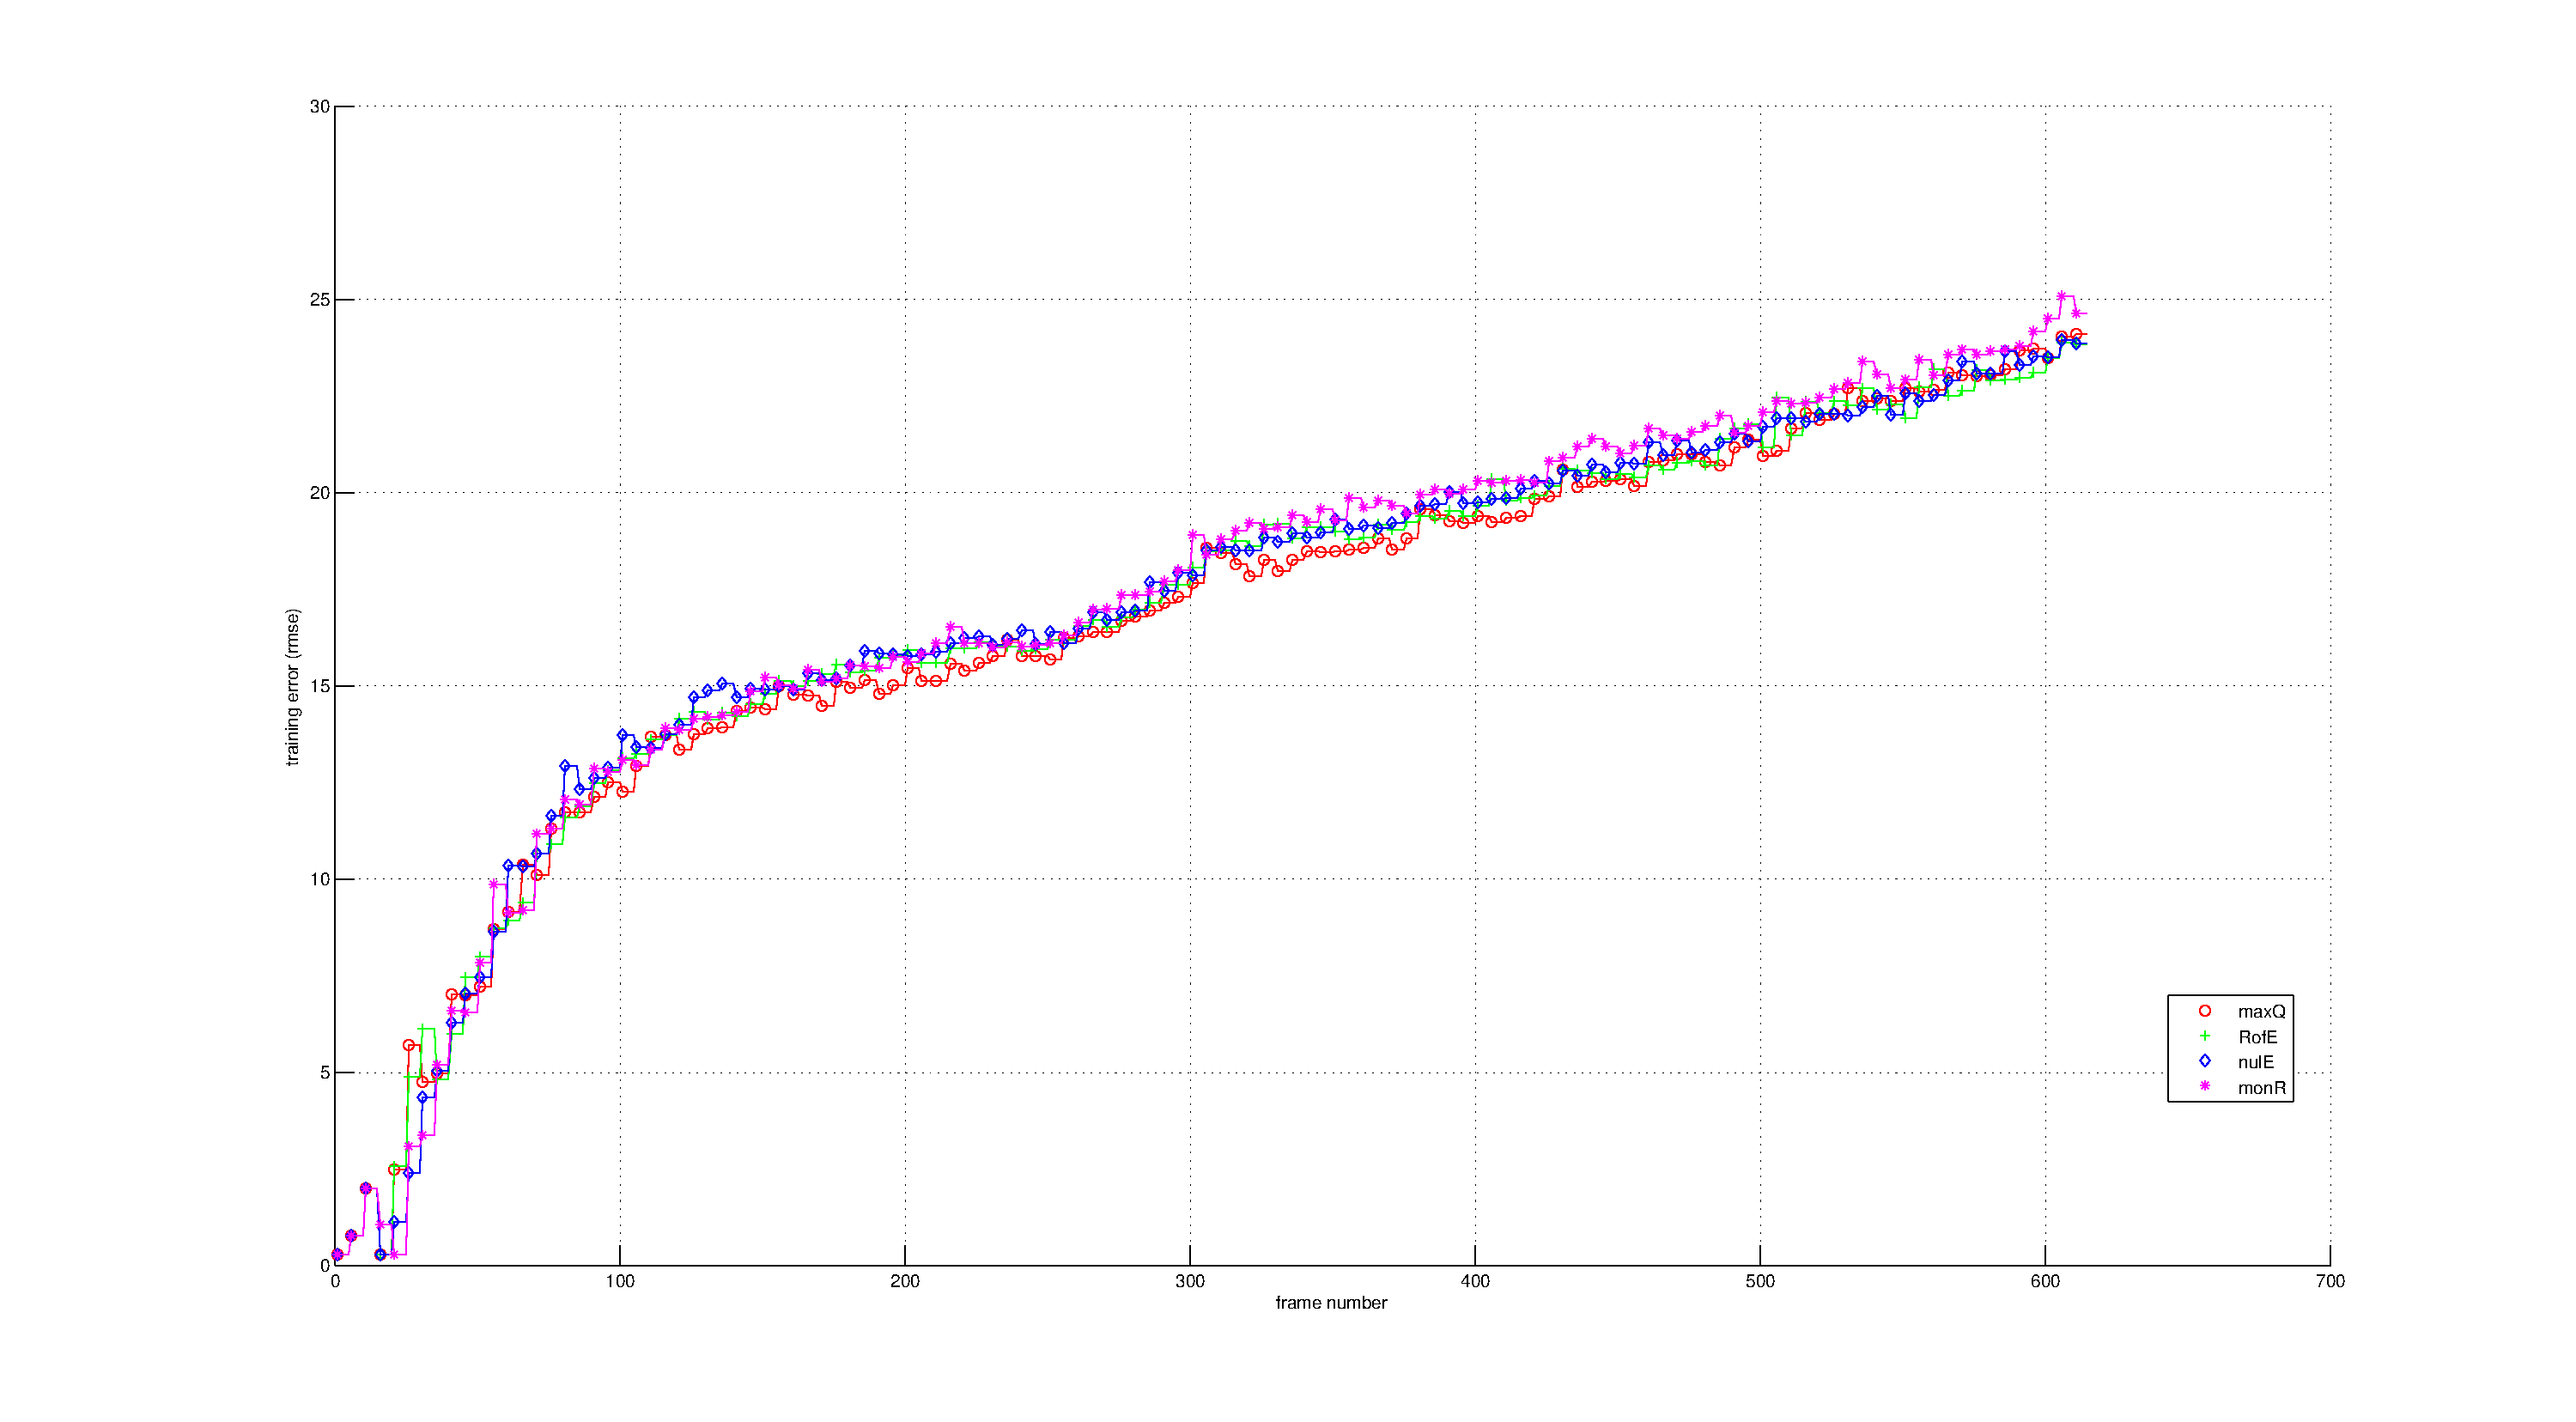
\includegraphics[height=0.4\textheight]{figs/3_sylv_8_4_1000_trg_rmse.pdf}
								\caption{8x4 RVQ, training error (rmse).}
								\label{fig:3_sylv_8_4_1000_trg_rmse}
								\end{figure}


								\begin{figure}[h!]
								\centering
								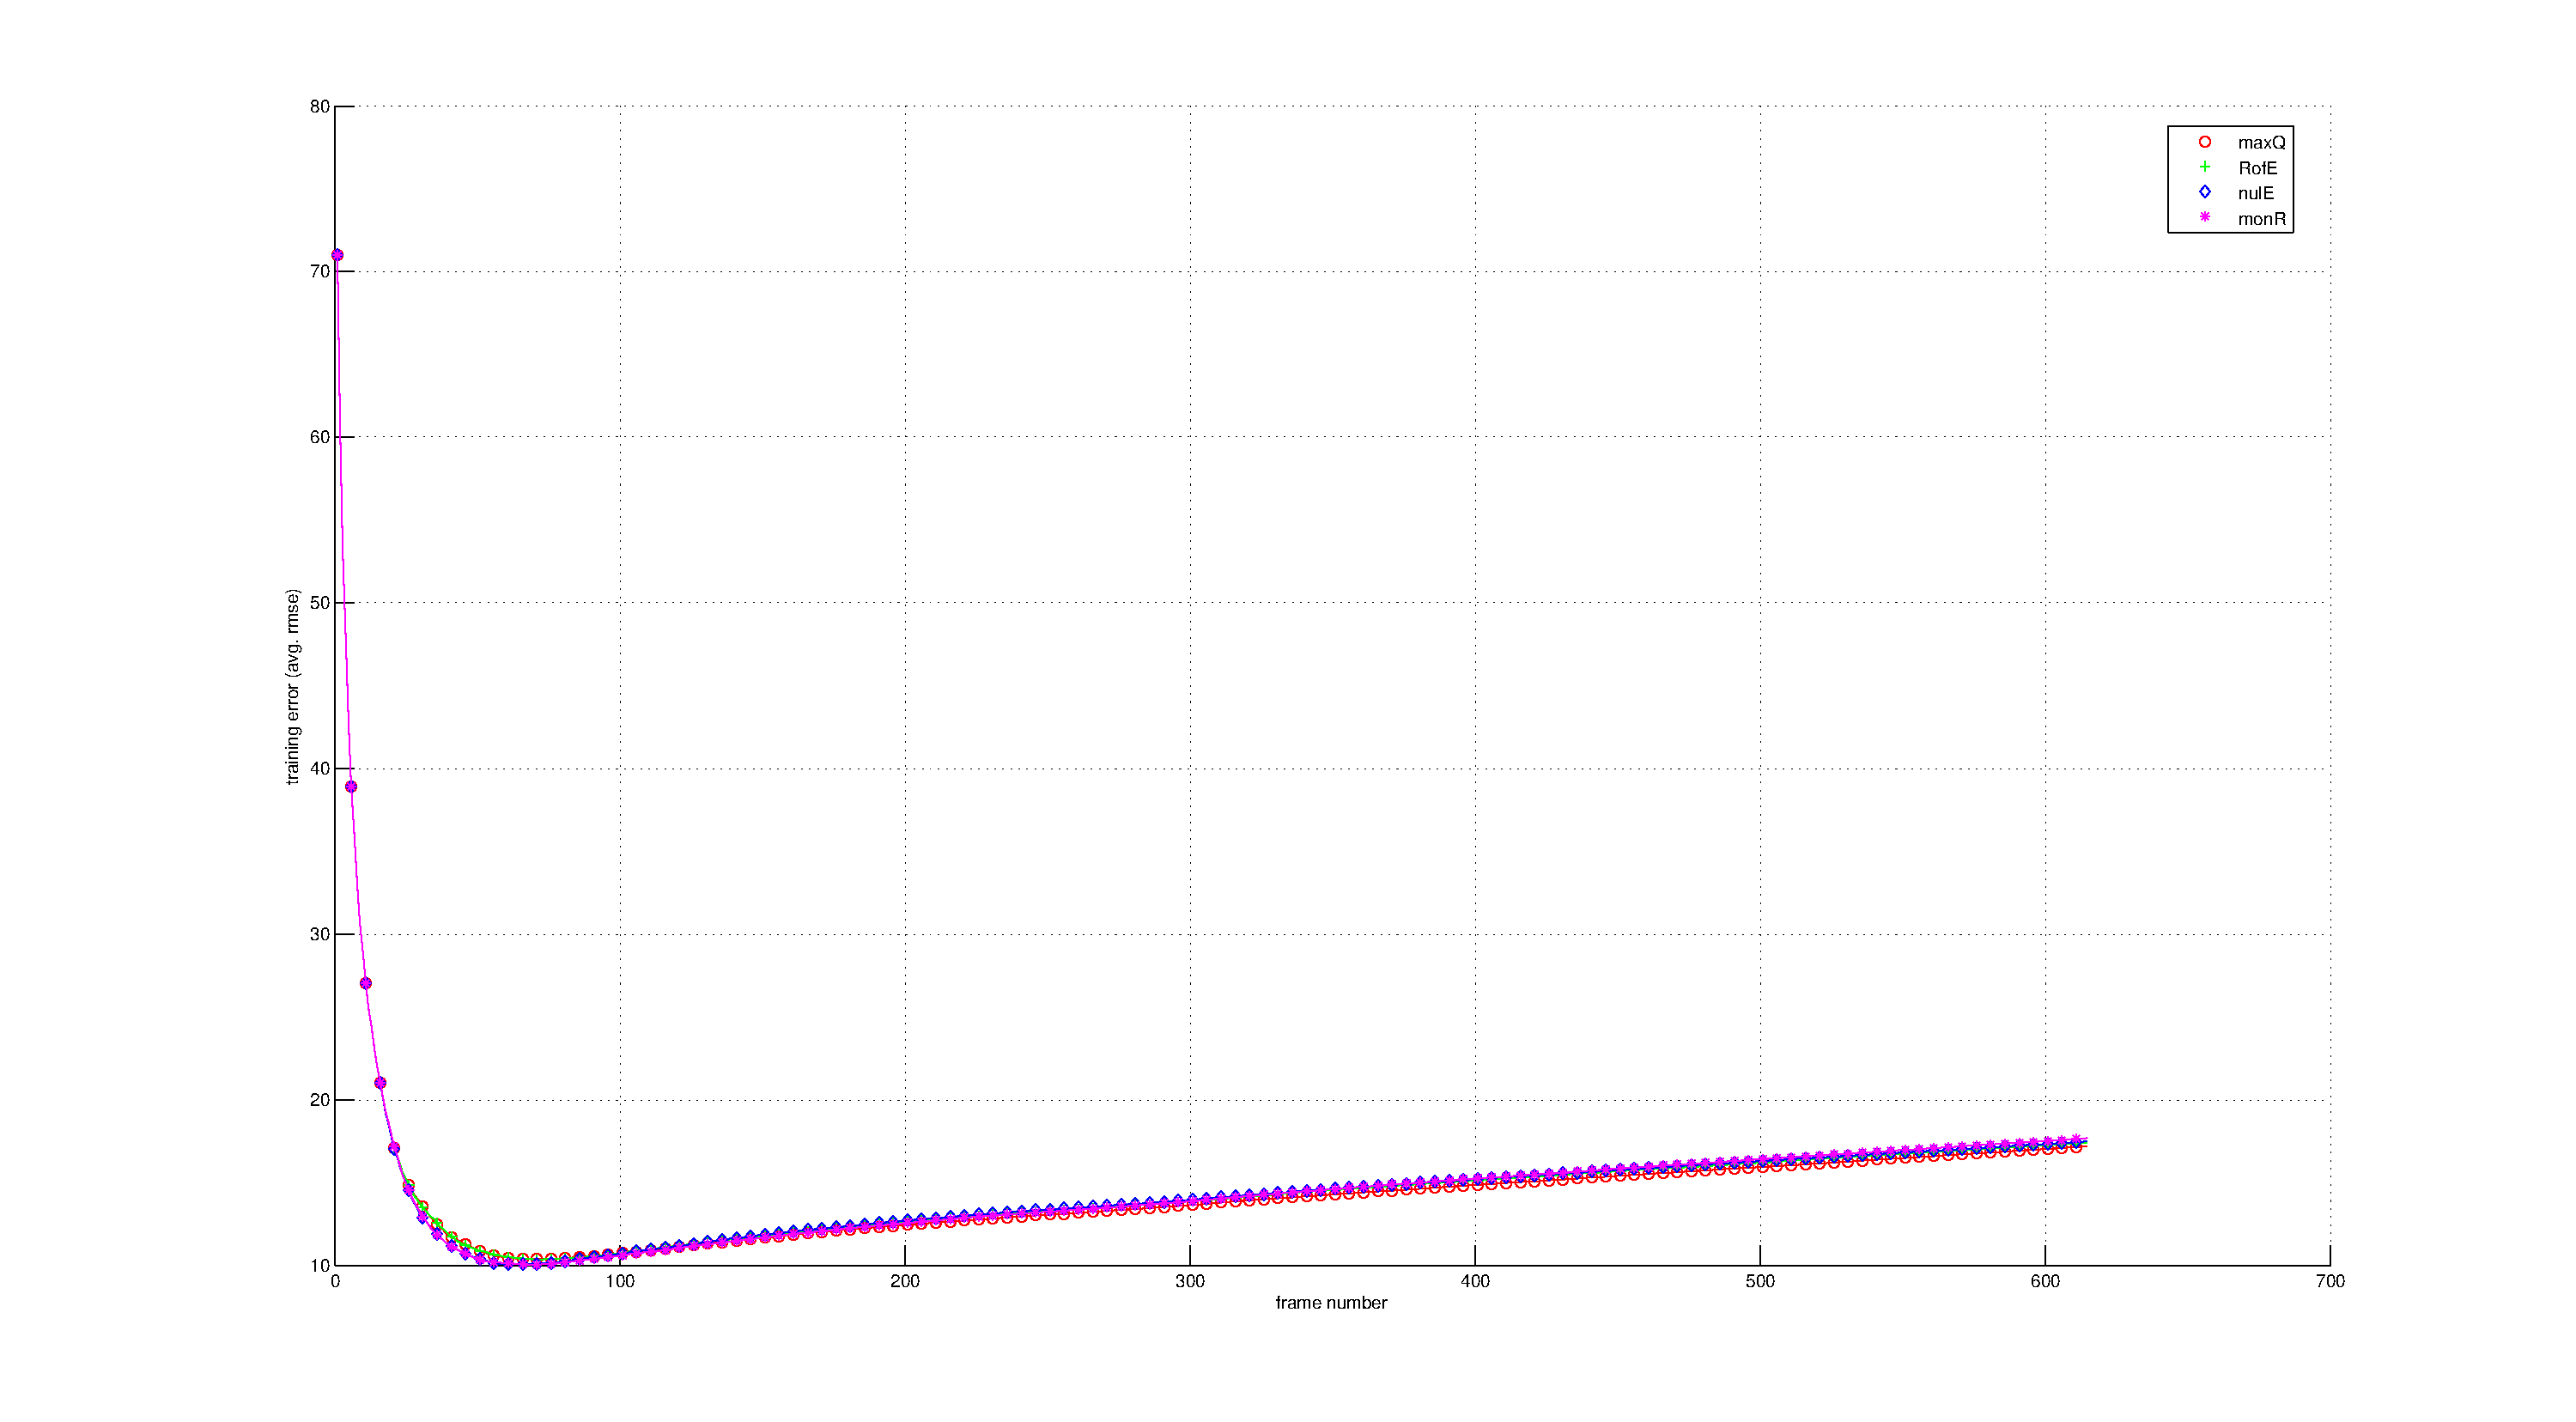
\includegraphics[height=0.4\textheight]{figs/3_sylv_8_4_1000_trg_armse.pdf}
								\caption{8x4 RVQ, training error (avg. rmse).}
								\label{fig:3_sylv_8_4_1000_trg_armse}
								\end{figure}

								\begin{figure}[h!]
								\centering
								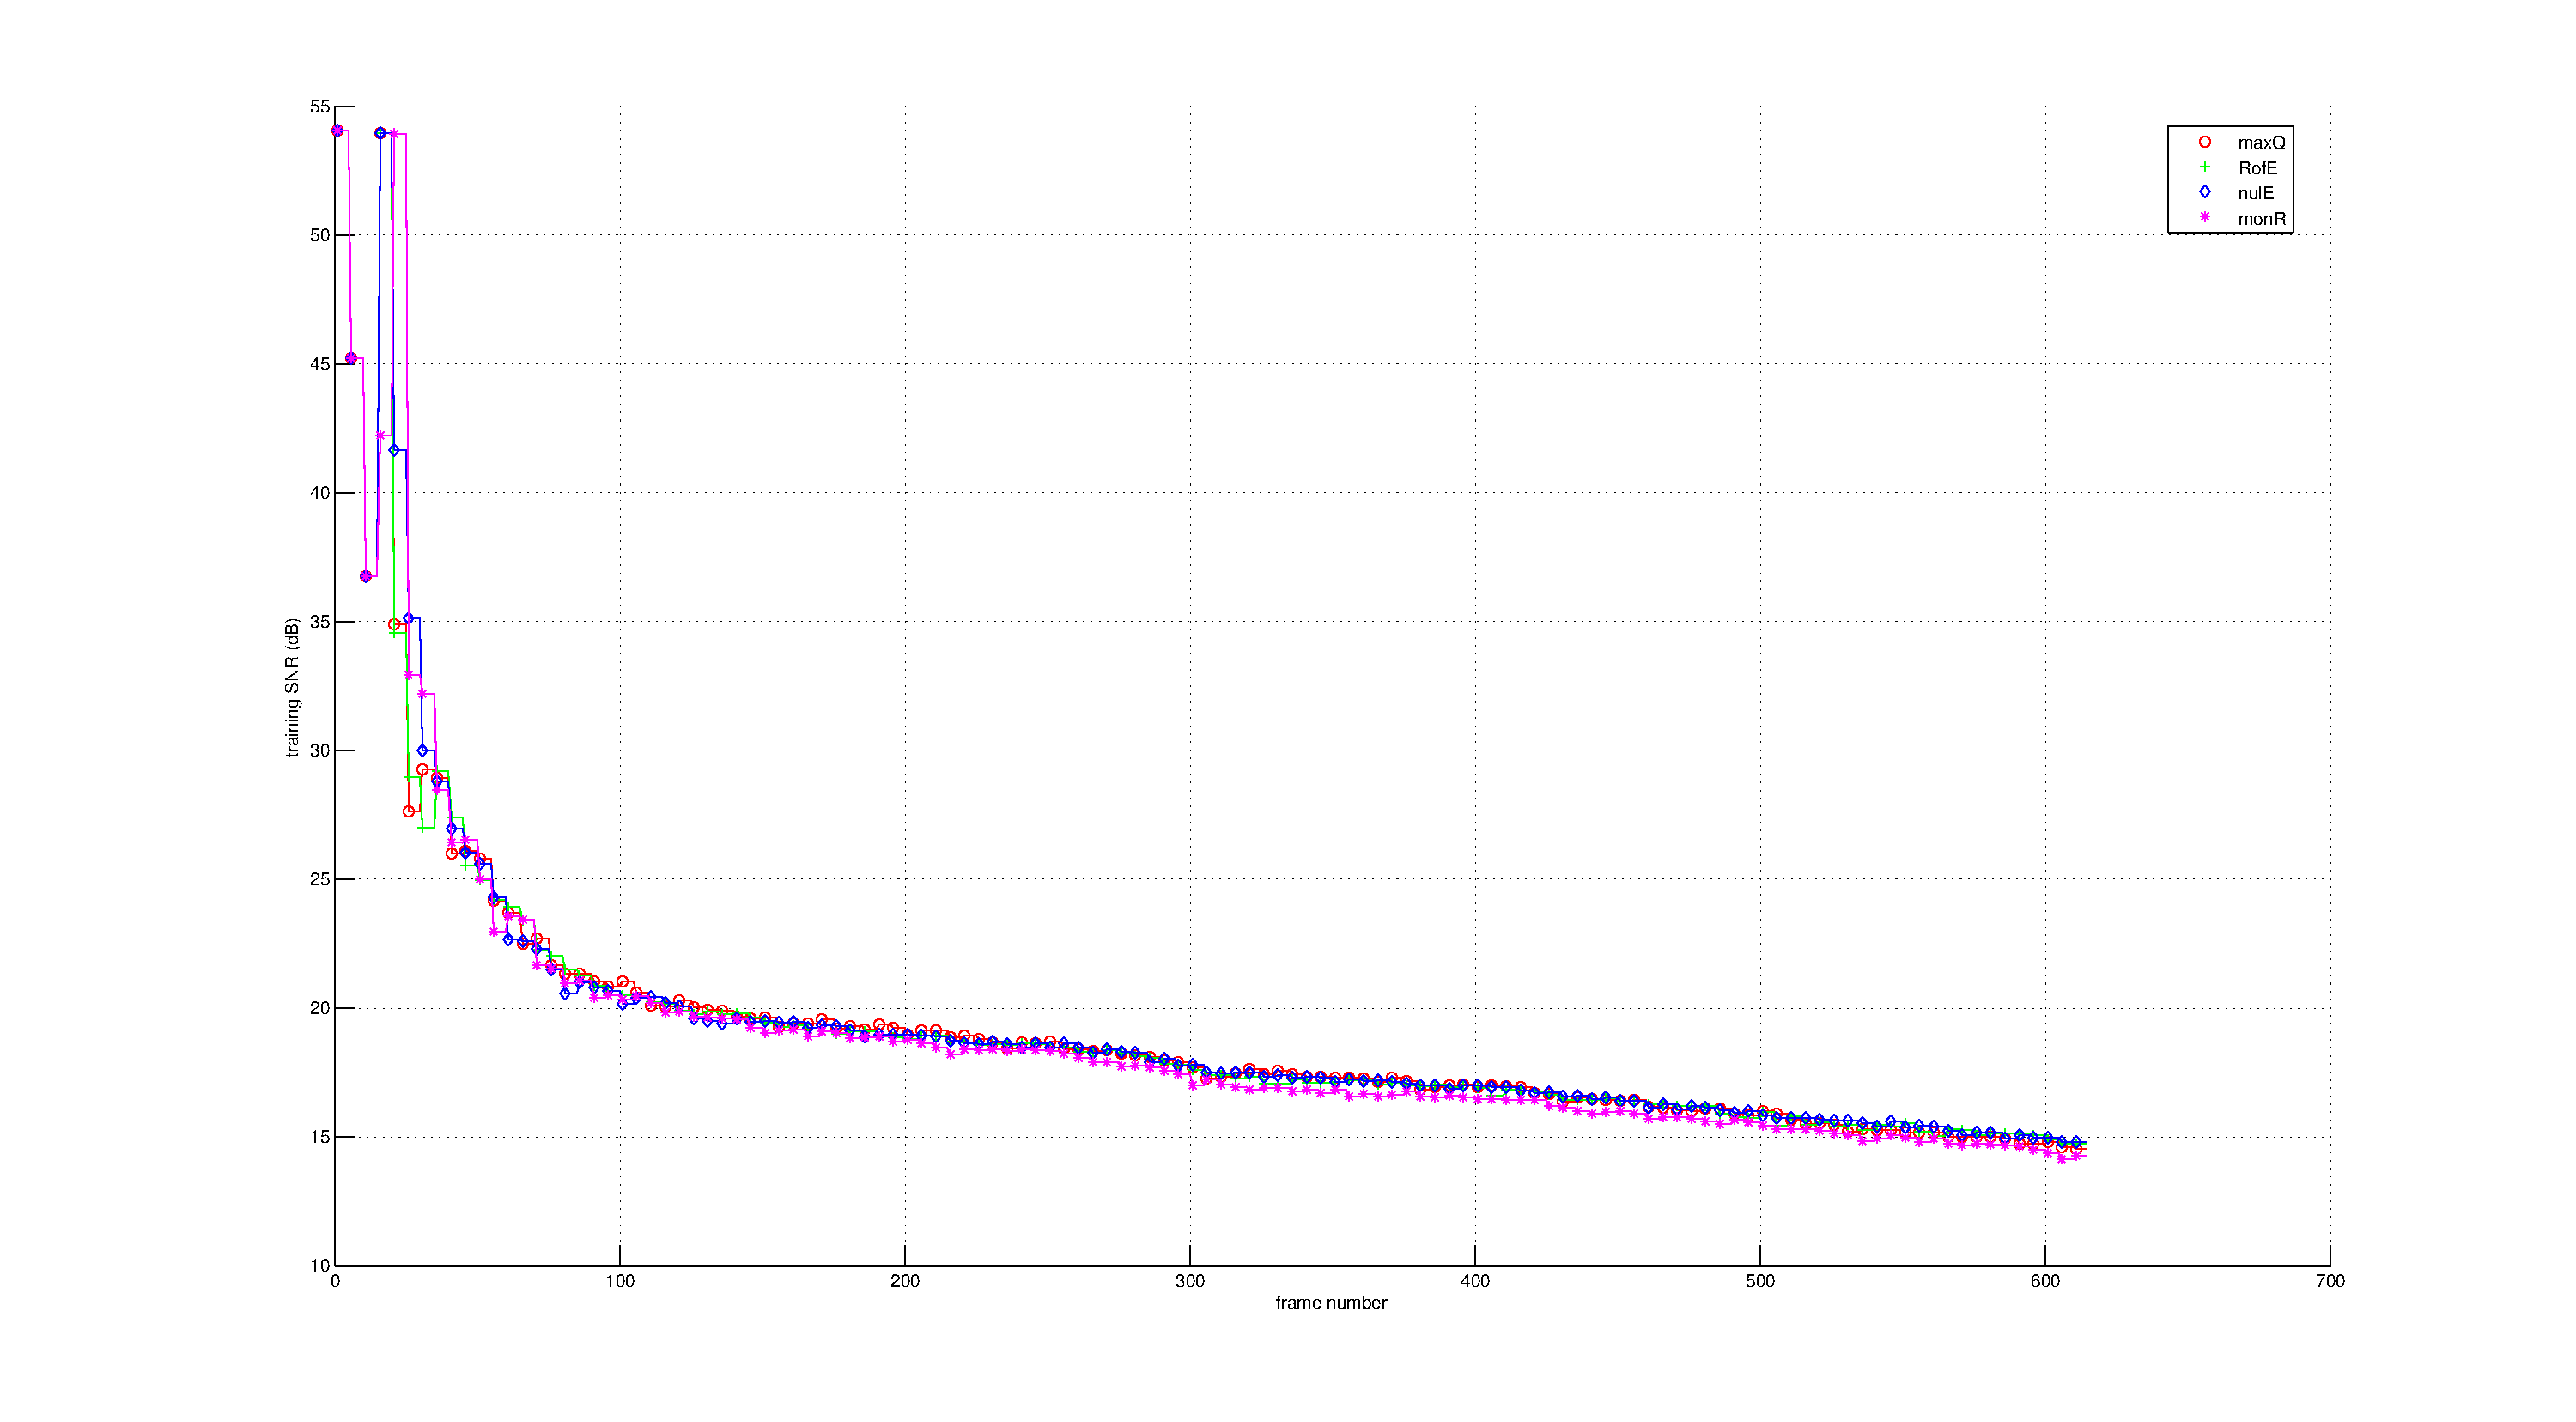
\includegraphics[height=0.4\textheight]{figs/3_sylv_8_4_1000_trg_SNRdB.pdf}
								\caption{8x4 RVQ, training SNR in dB.}
								\label{fig:3_sylv_8_4_1000_trg_SNRdB}
								\end{figure}
%------------------------------------
\clearpage
\newpage
\subsection{Testing}
%------------------------------------
								\begin{figure}[h!]
								\centering
								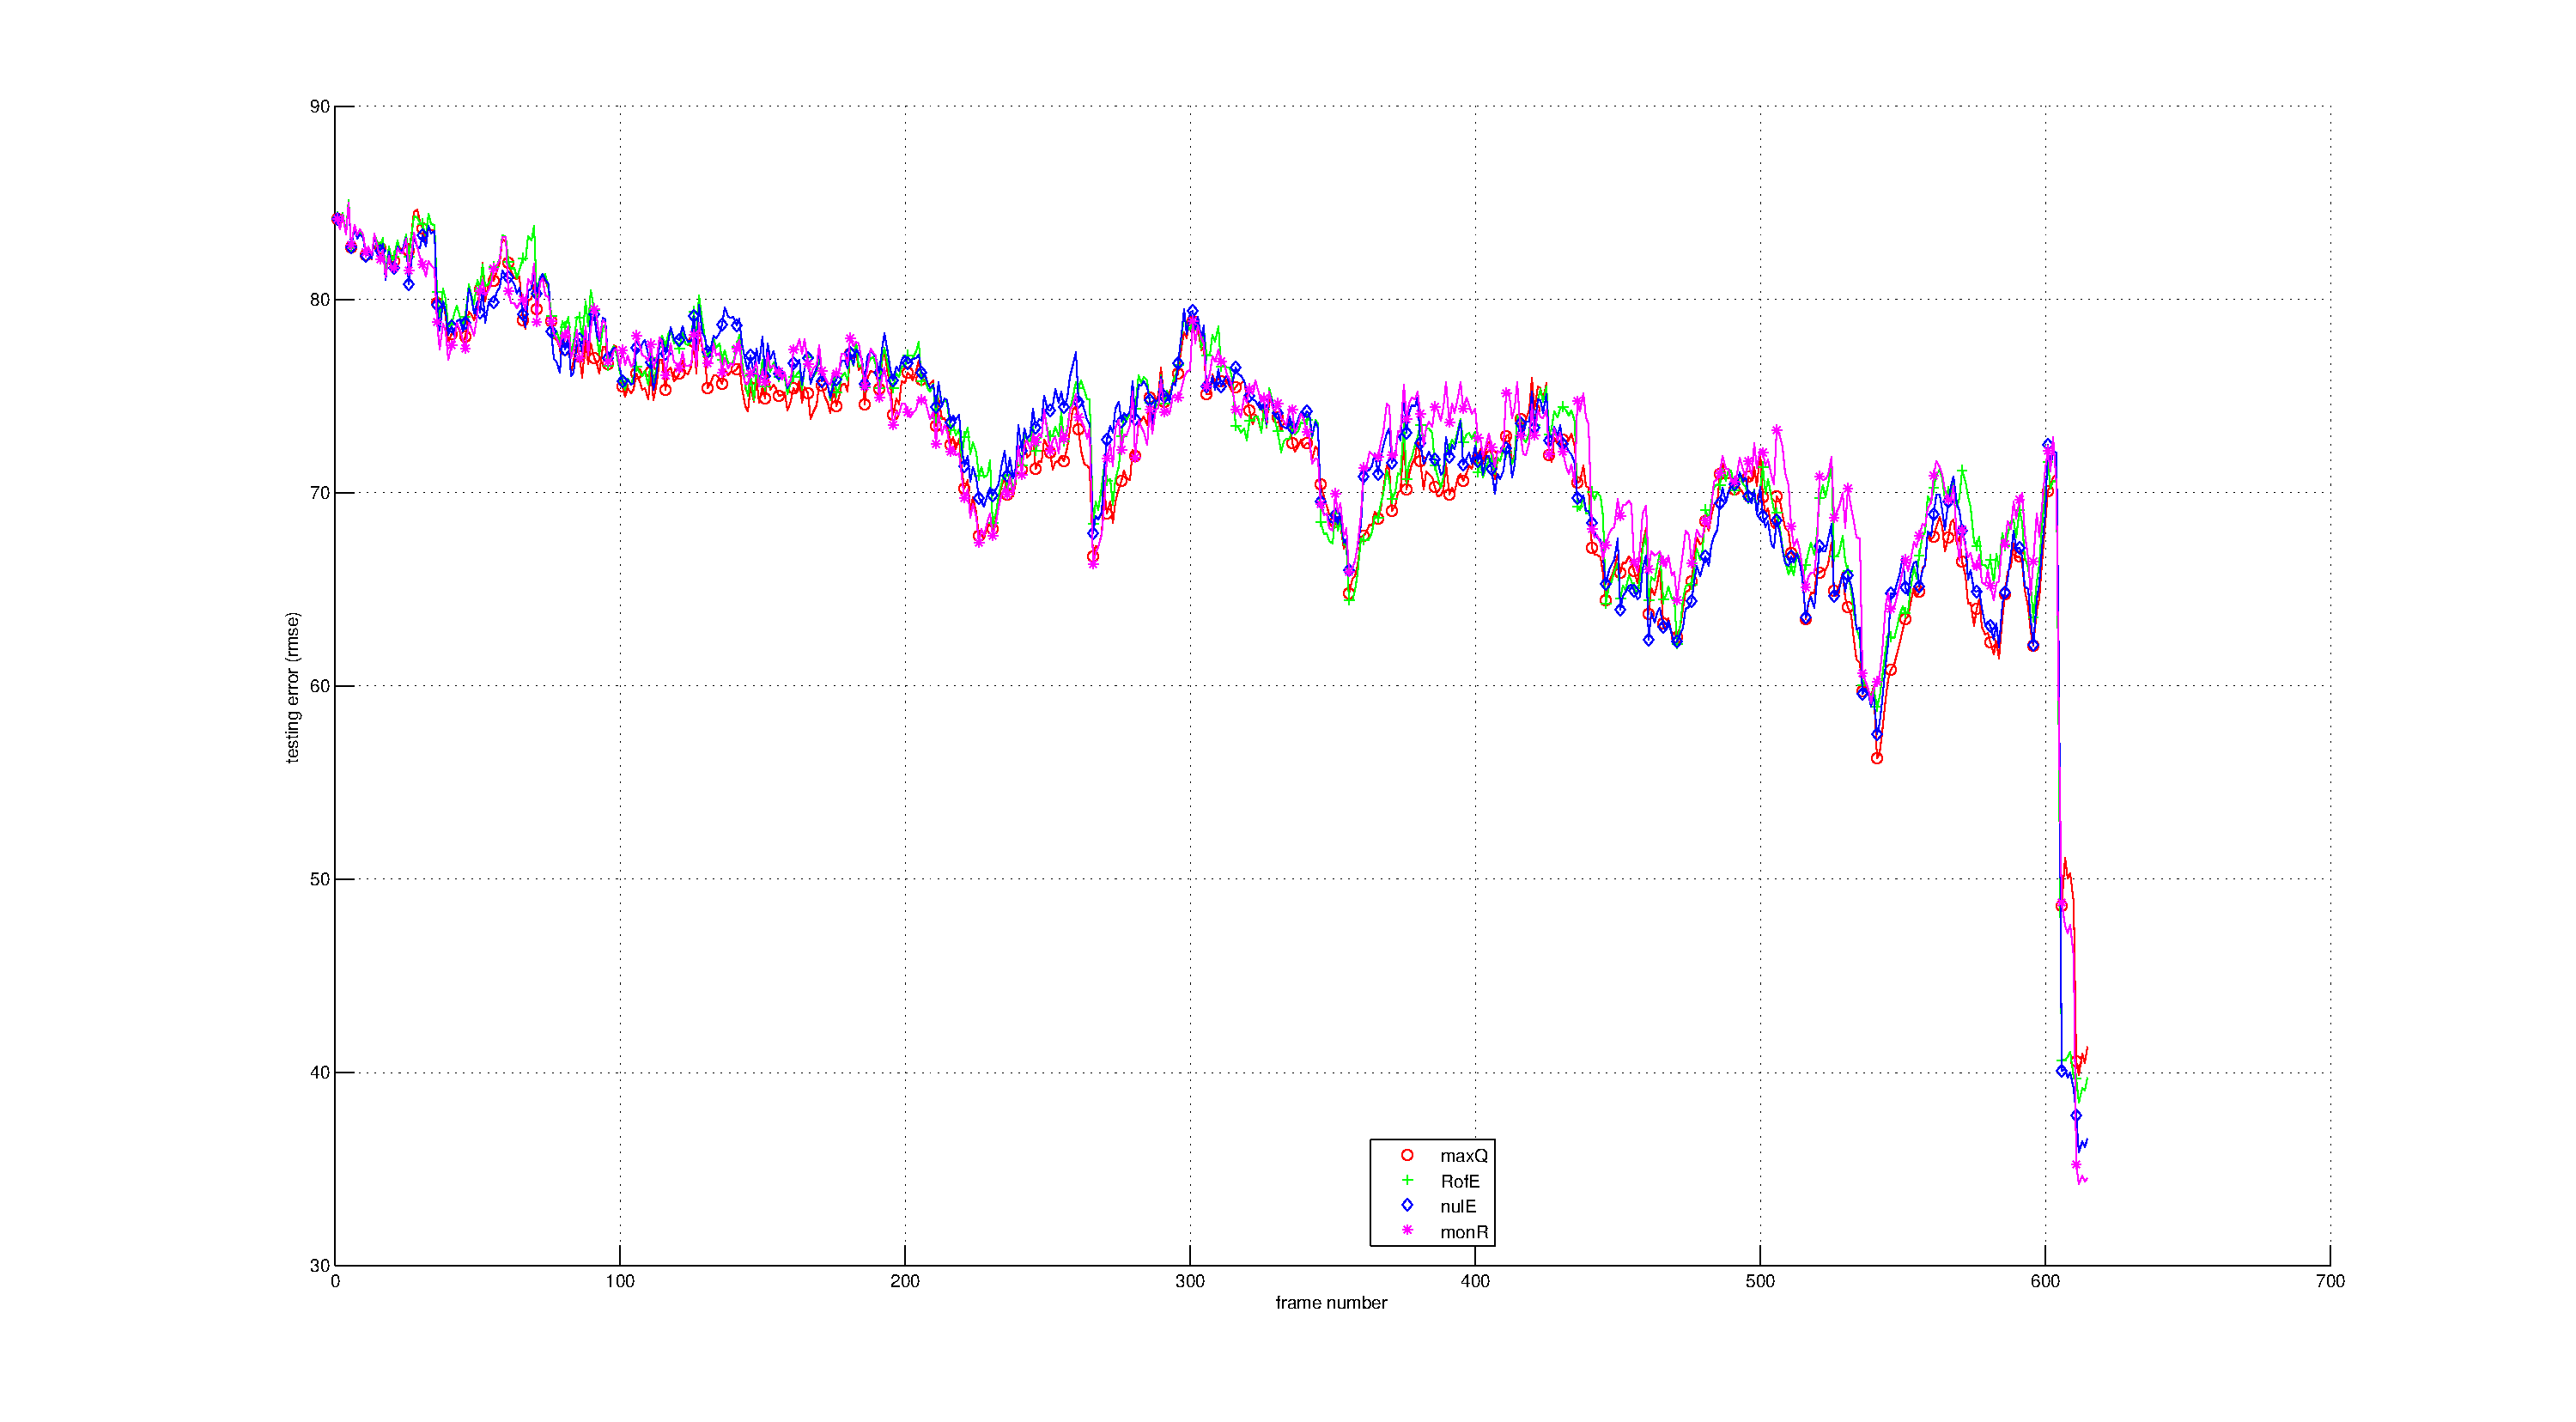
\includegraphics[height=0.4\textheight]{figs/3_sylv_8_4_1000_tst_rmse.pdf}
								\caption{8x4 RVQ, testing error (rmse).}
								\label{fig:3_sylv_8_4_1000_tst_rmse}
								\end{figure}


								\begin{figure}[h!]
								\centering
								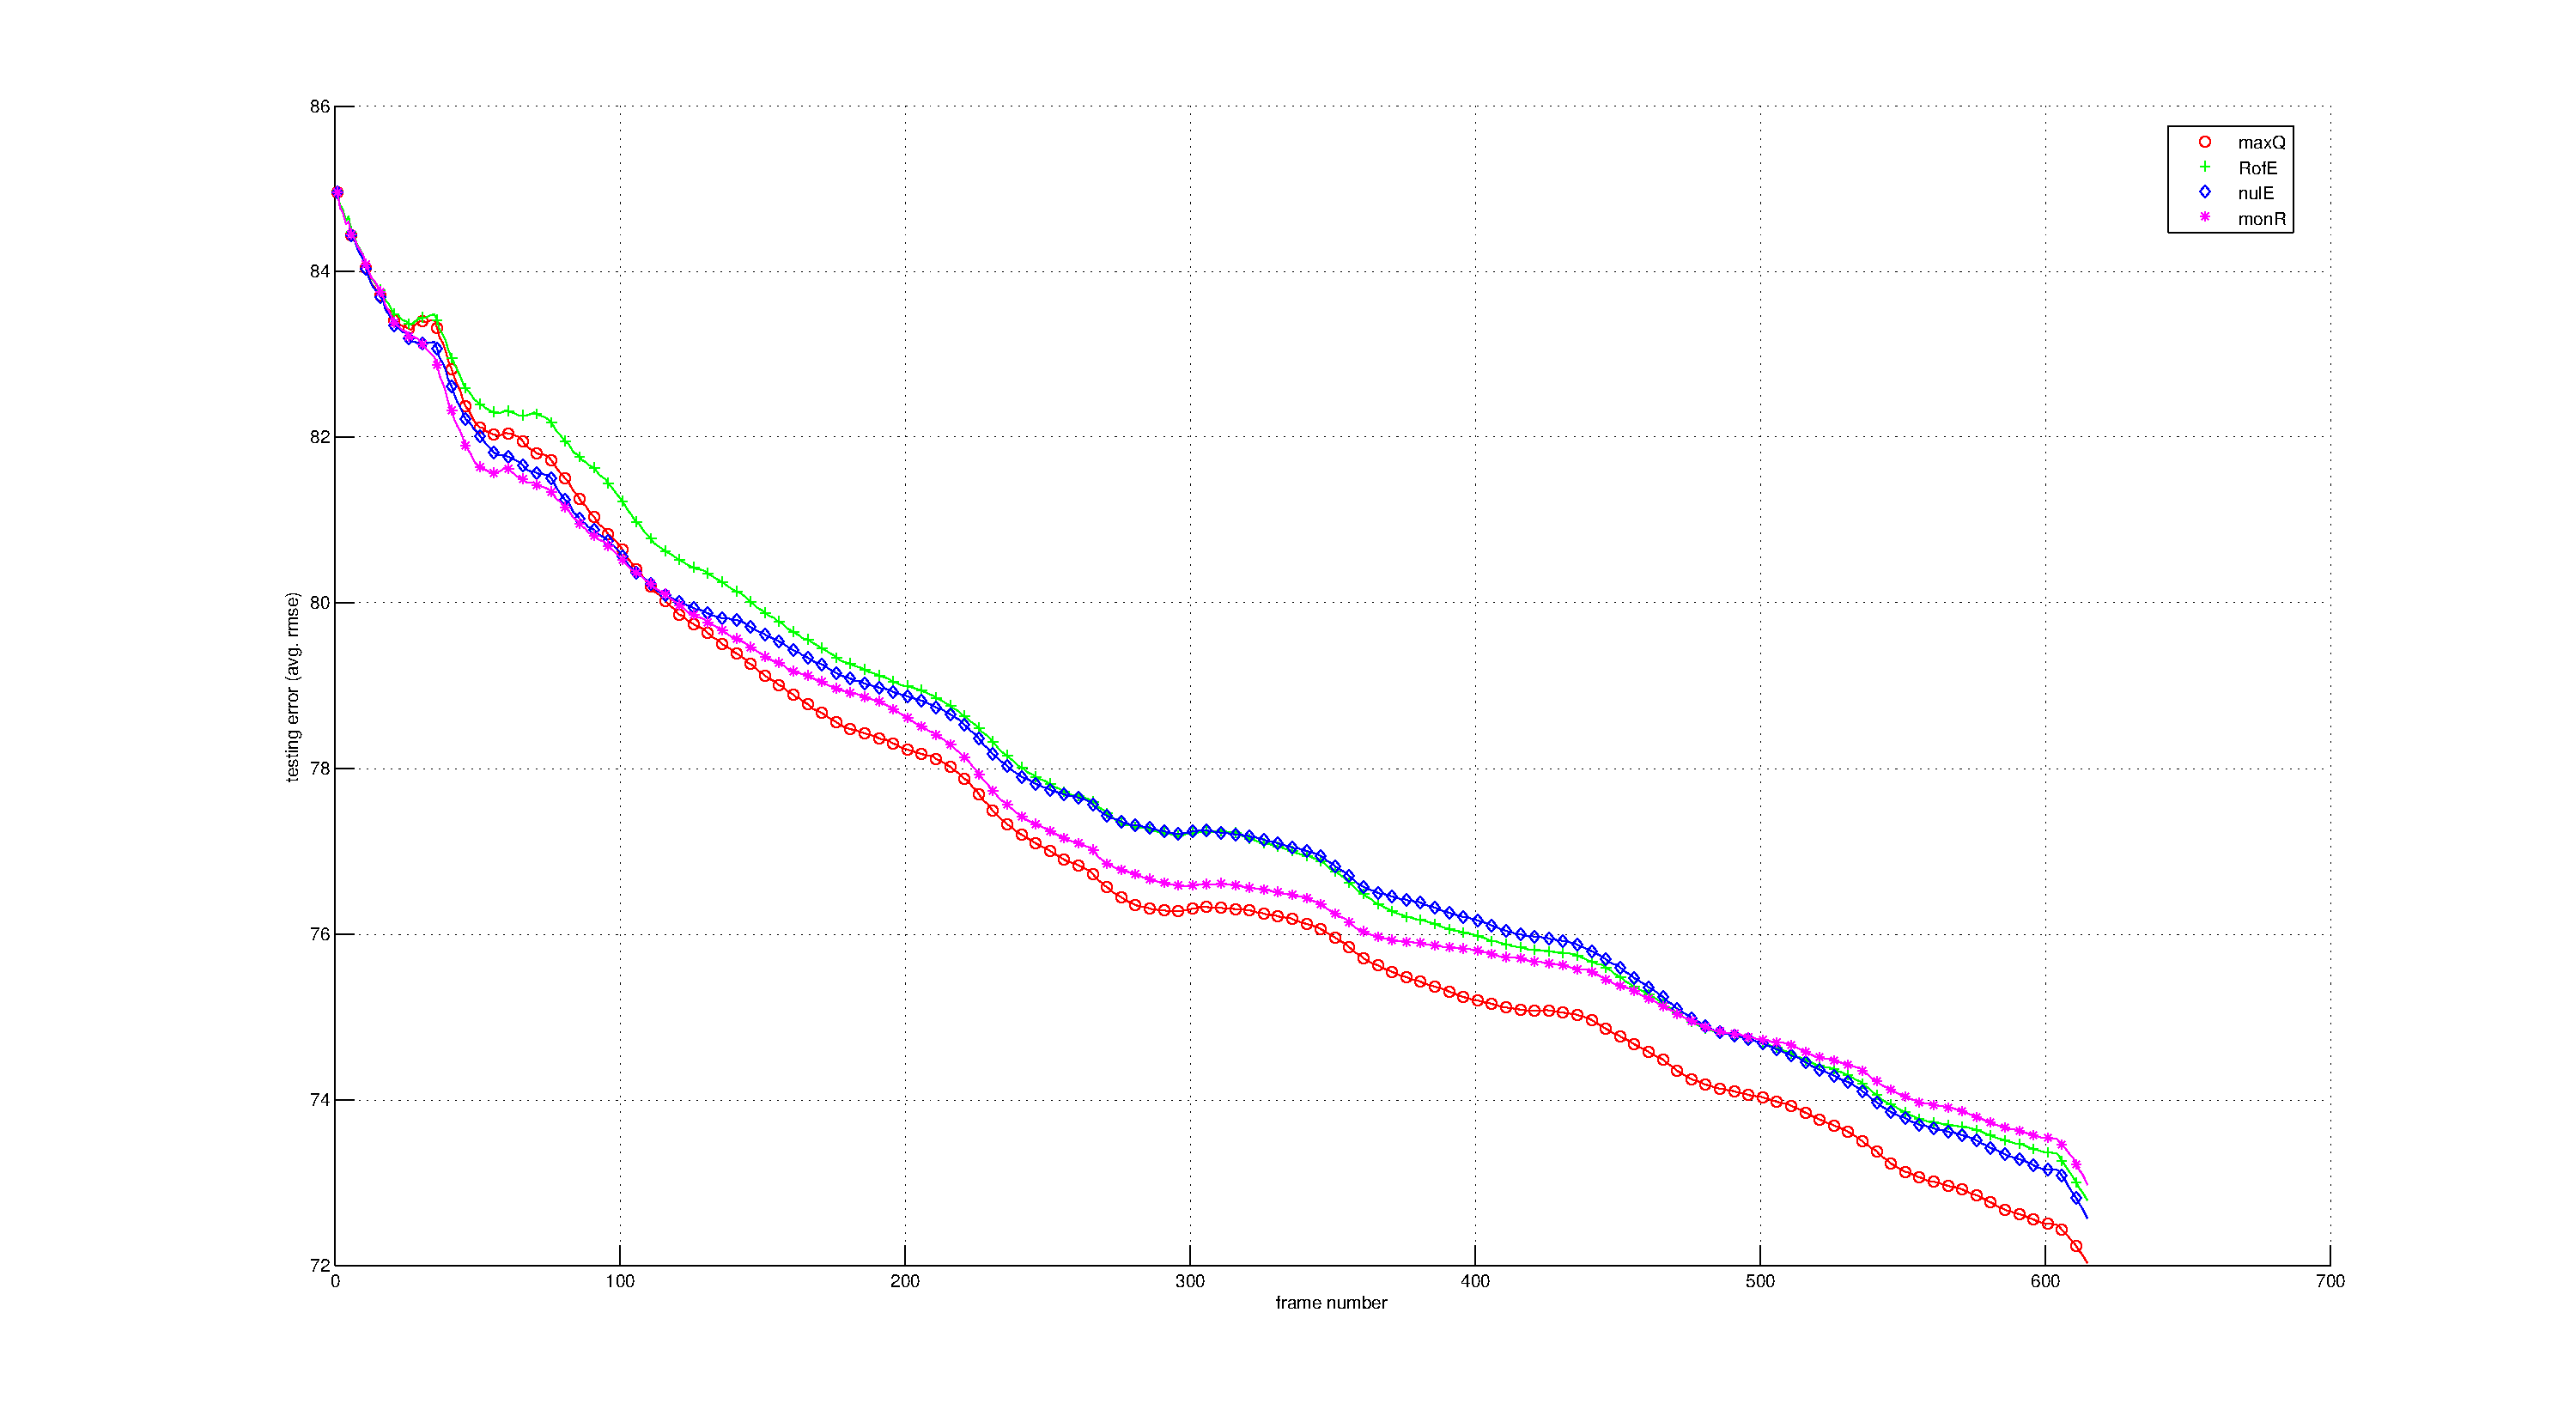
\includegraphics[height=0.4\textheight]{figs/3_sylv_8_4_1000_tst_armse.pdf}
								\caption{8x4 RVQ, testing error (avg. rmse).}
								\label{fig:3_sylv_8_4_1000_tst_armse}
								\end{figure}

								\begin{figure}[h!]
								\centering
								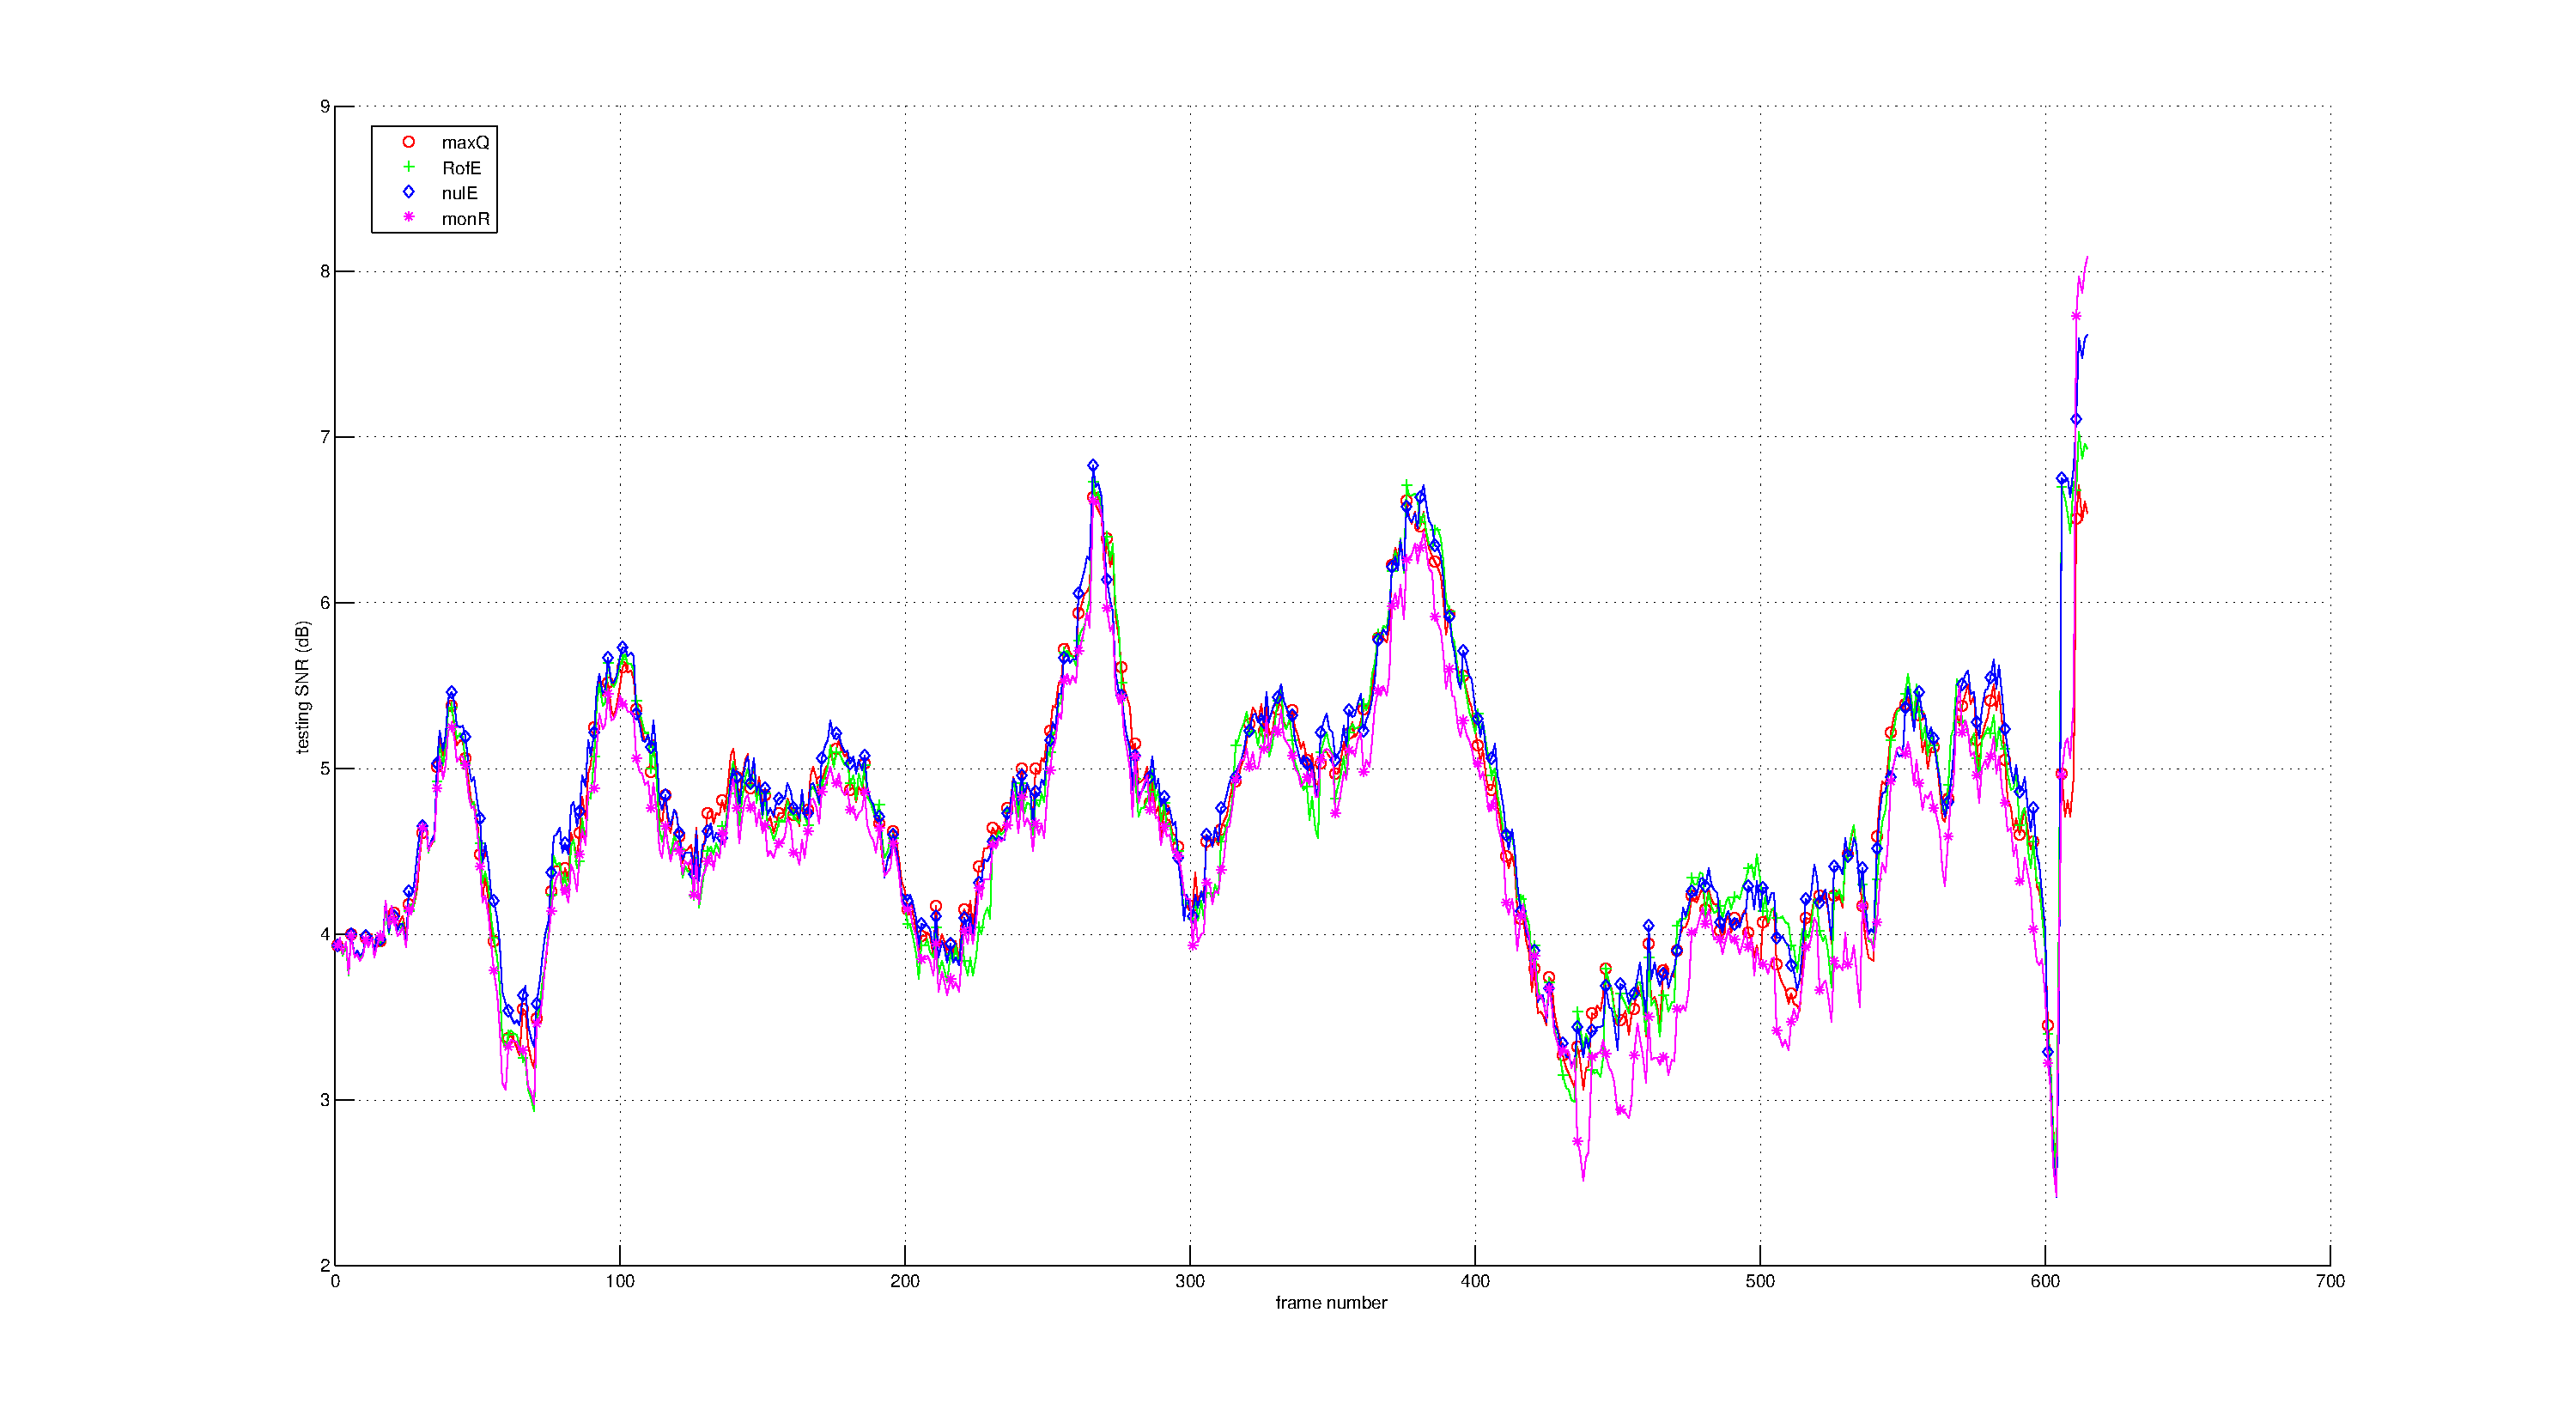
\includegraphics[height=0.4\textheight]{figs/3_sylv_8_4_1000_tst_SNRdB.pdf}
								\caption{8x4 RVQ,testing SNR in dB.}
								\label{fig:3_sylv_8_4_1000_tst_SNRdB}
								\end{figure}

%%%===============================
\clearpage
\newpage
\section{Tracking: trellis70 dataset} 
%===============================
								\begin{figure}[h]
								\centering
								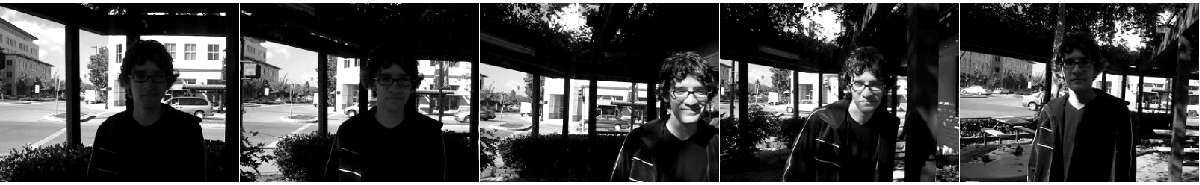
\includegraphics[width=1.0\textwidth]{thesis/seq_4_trellis70.png}
								\caption{trellis70 dataset.}
								\label{fig:seq_4_trellis70}
								\end{figure}



\begin{table}[h]
\centering
\input{thesis/tables_4_trellis70_rvq.tex}
\caption{Tracking errors for various RVQ configurations.  -1 means that track was lost.  These results show that RVQ is able to track the object of interest very closely.}
\end{table}

For the interested reader, detailed graphical results follow for 8x4 RVQ.
%------------------------------------
\clearpage
\newpage
\subsection{Tracking error}
%------------------------------------

								\begin{figure}[h!]
								\centering
								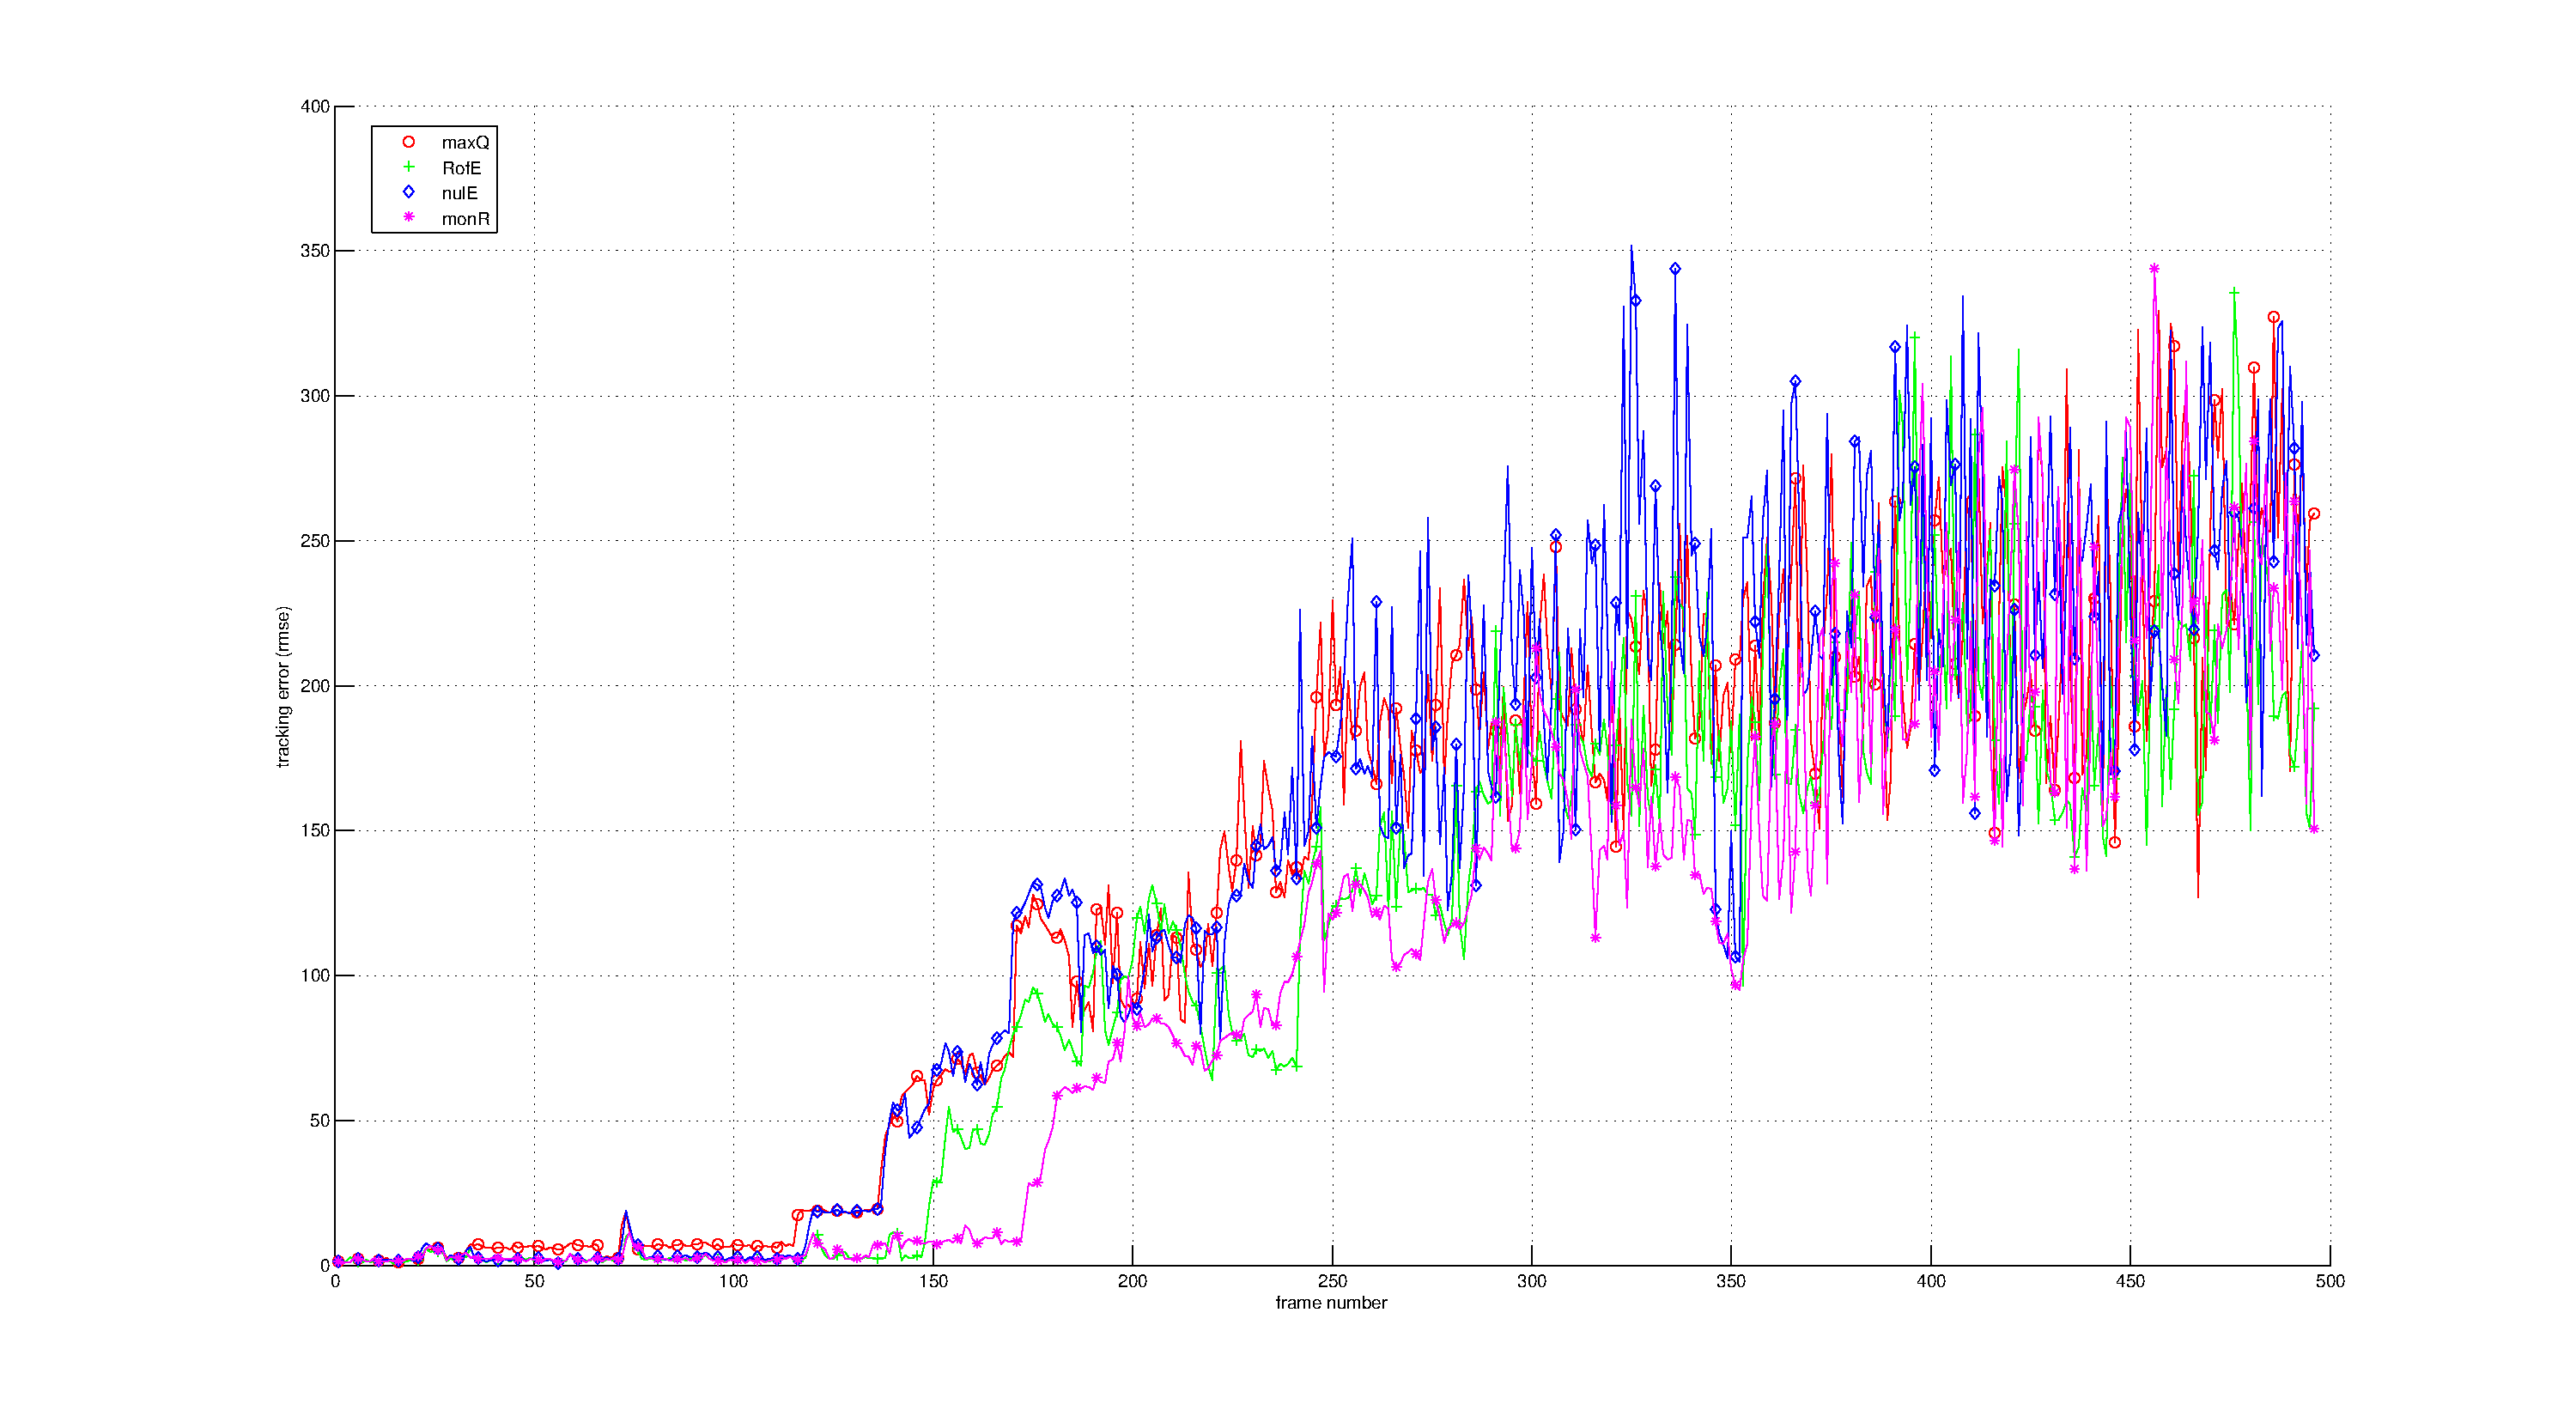
\includegraphics[height=0.38\textheight]{thesis/4_trellis70_8_4_1000_trk_rmse.pdf}
								\caption{8x4 RVQ, tracking error (rmse).}
								\label{fig:4_trellis70_8_4_1000_trk_rmse}
								\end{figure}


								\begin{figure}[h!]
								\centering
								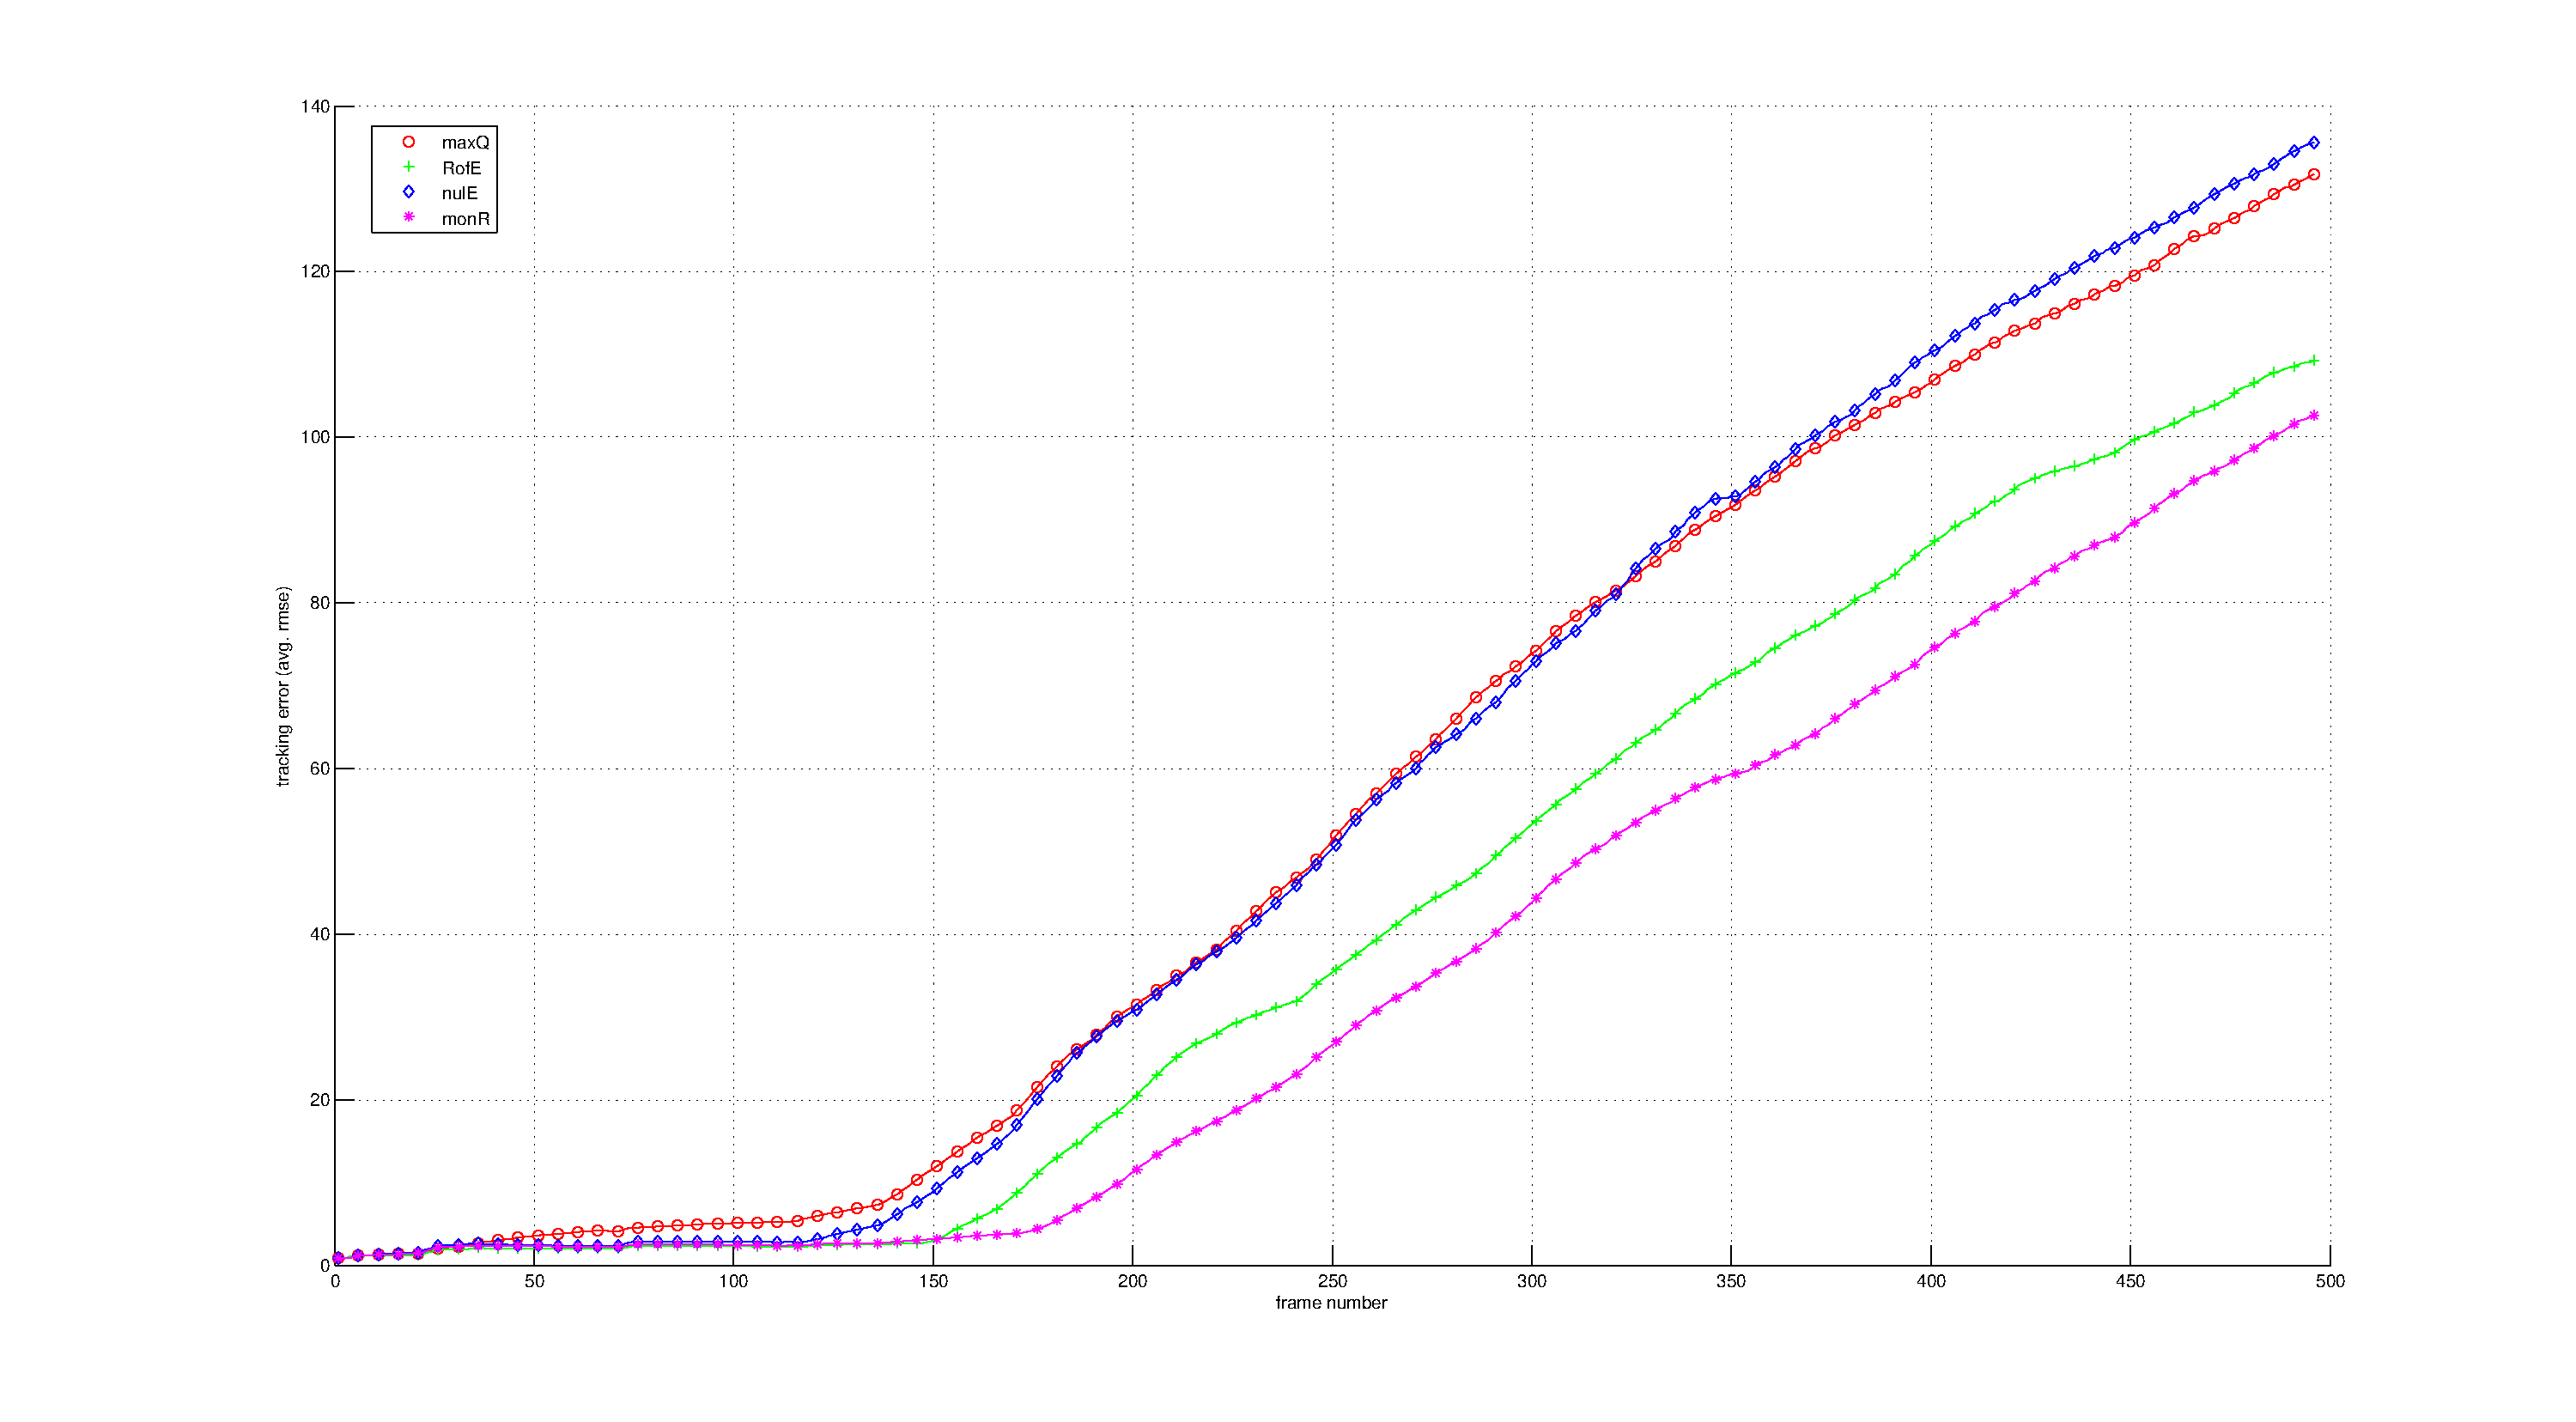
\includegraphics[height=0.38\textheight]{thesis/4_trellis70_8_4_1000_trk_armse.pdf}
								\caption{8x4 RVQ, tracking error (average rmse).}
								\label{fig:4_trellis70_8_4_1000_trk_avg_rmse}
								\end{figure}

%------------------------------------
\clearpage
\newpage
\subsection{Target reconstruction}
%------------------------------------

								\begin{figure}[h!]
								\centering
								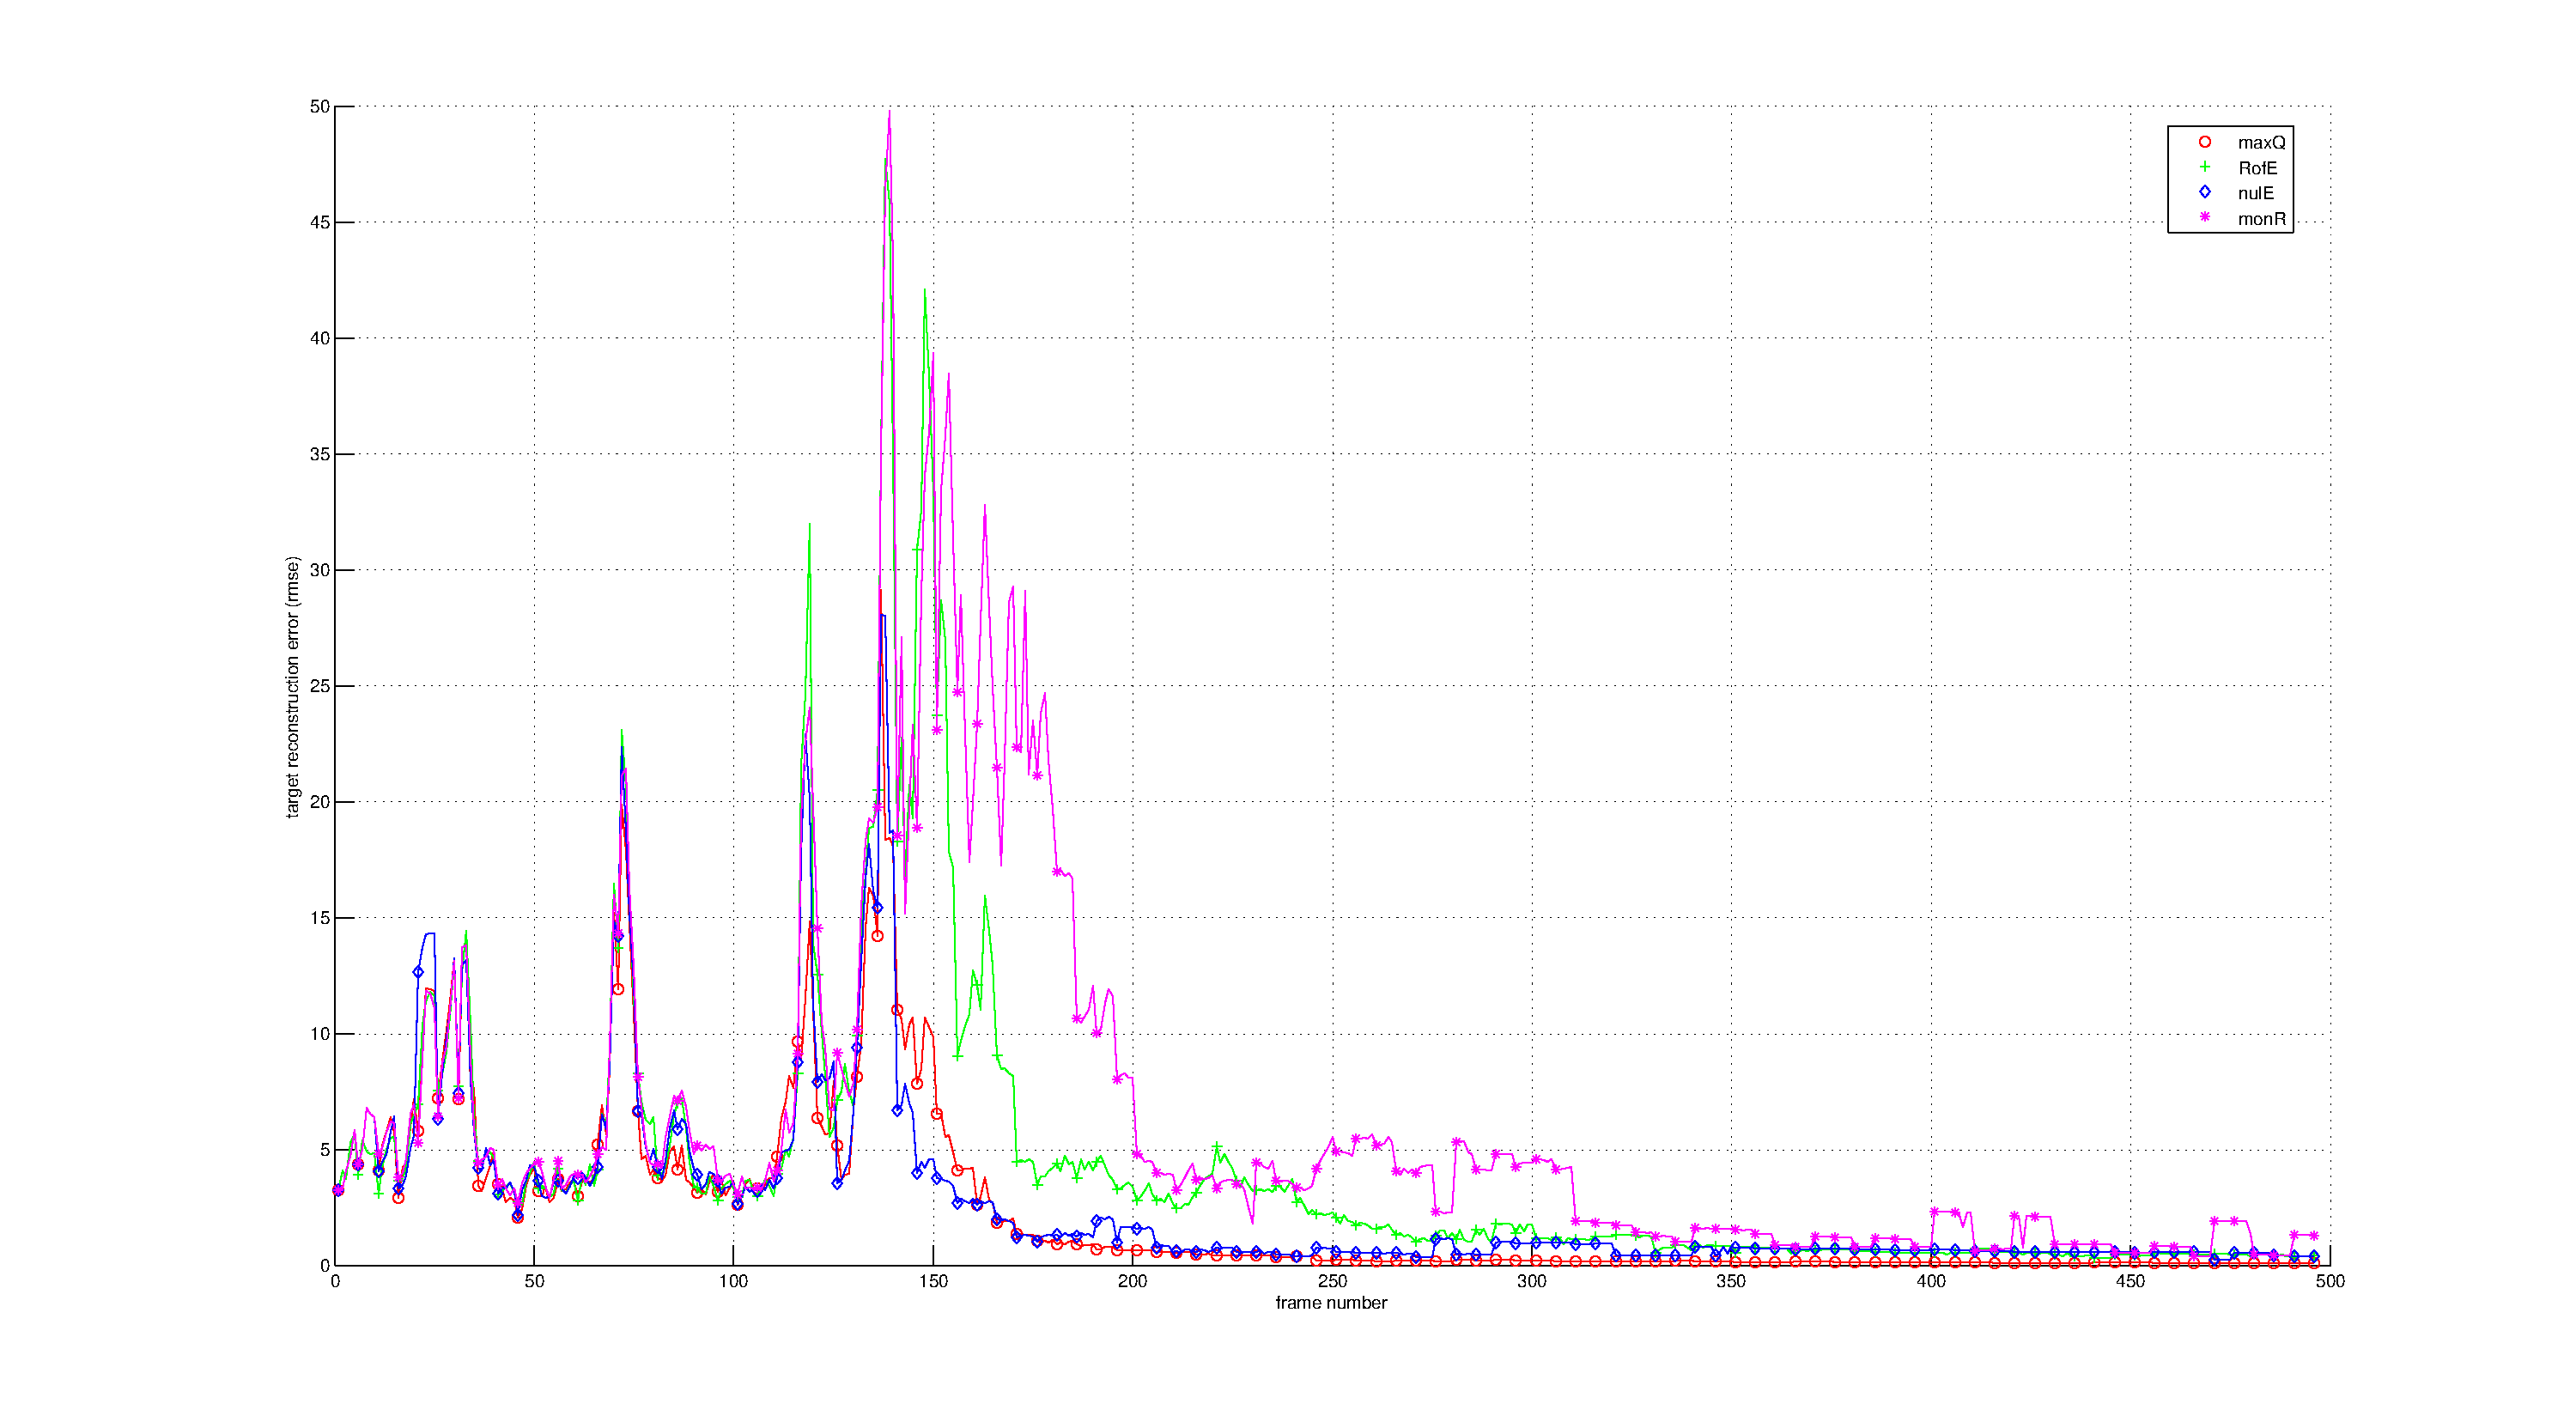
\includegraphics[height=0.4\textheight]{thesis/4_trellis70_8_4_1000_snp_rmse.pdf}
								\caption{8x4 RVQ, snippet reconstruction error (rmse).}
								\label{fig:4_trellis70_8_4_1000_snp_rmse}
								\end{figure}


								\begin{figure}[h!]
								\centering
								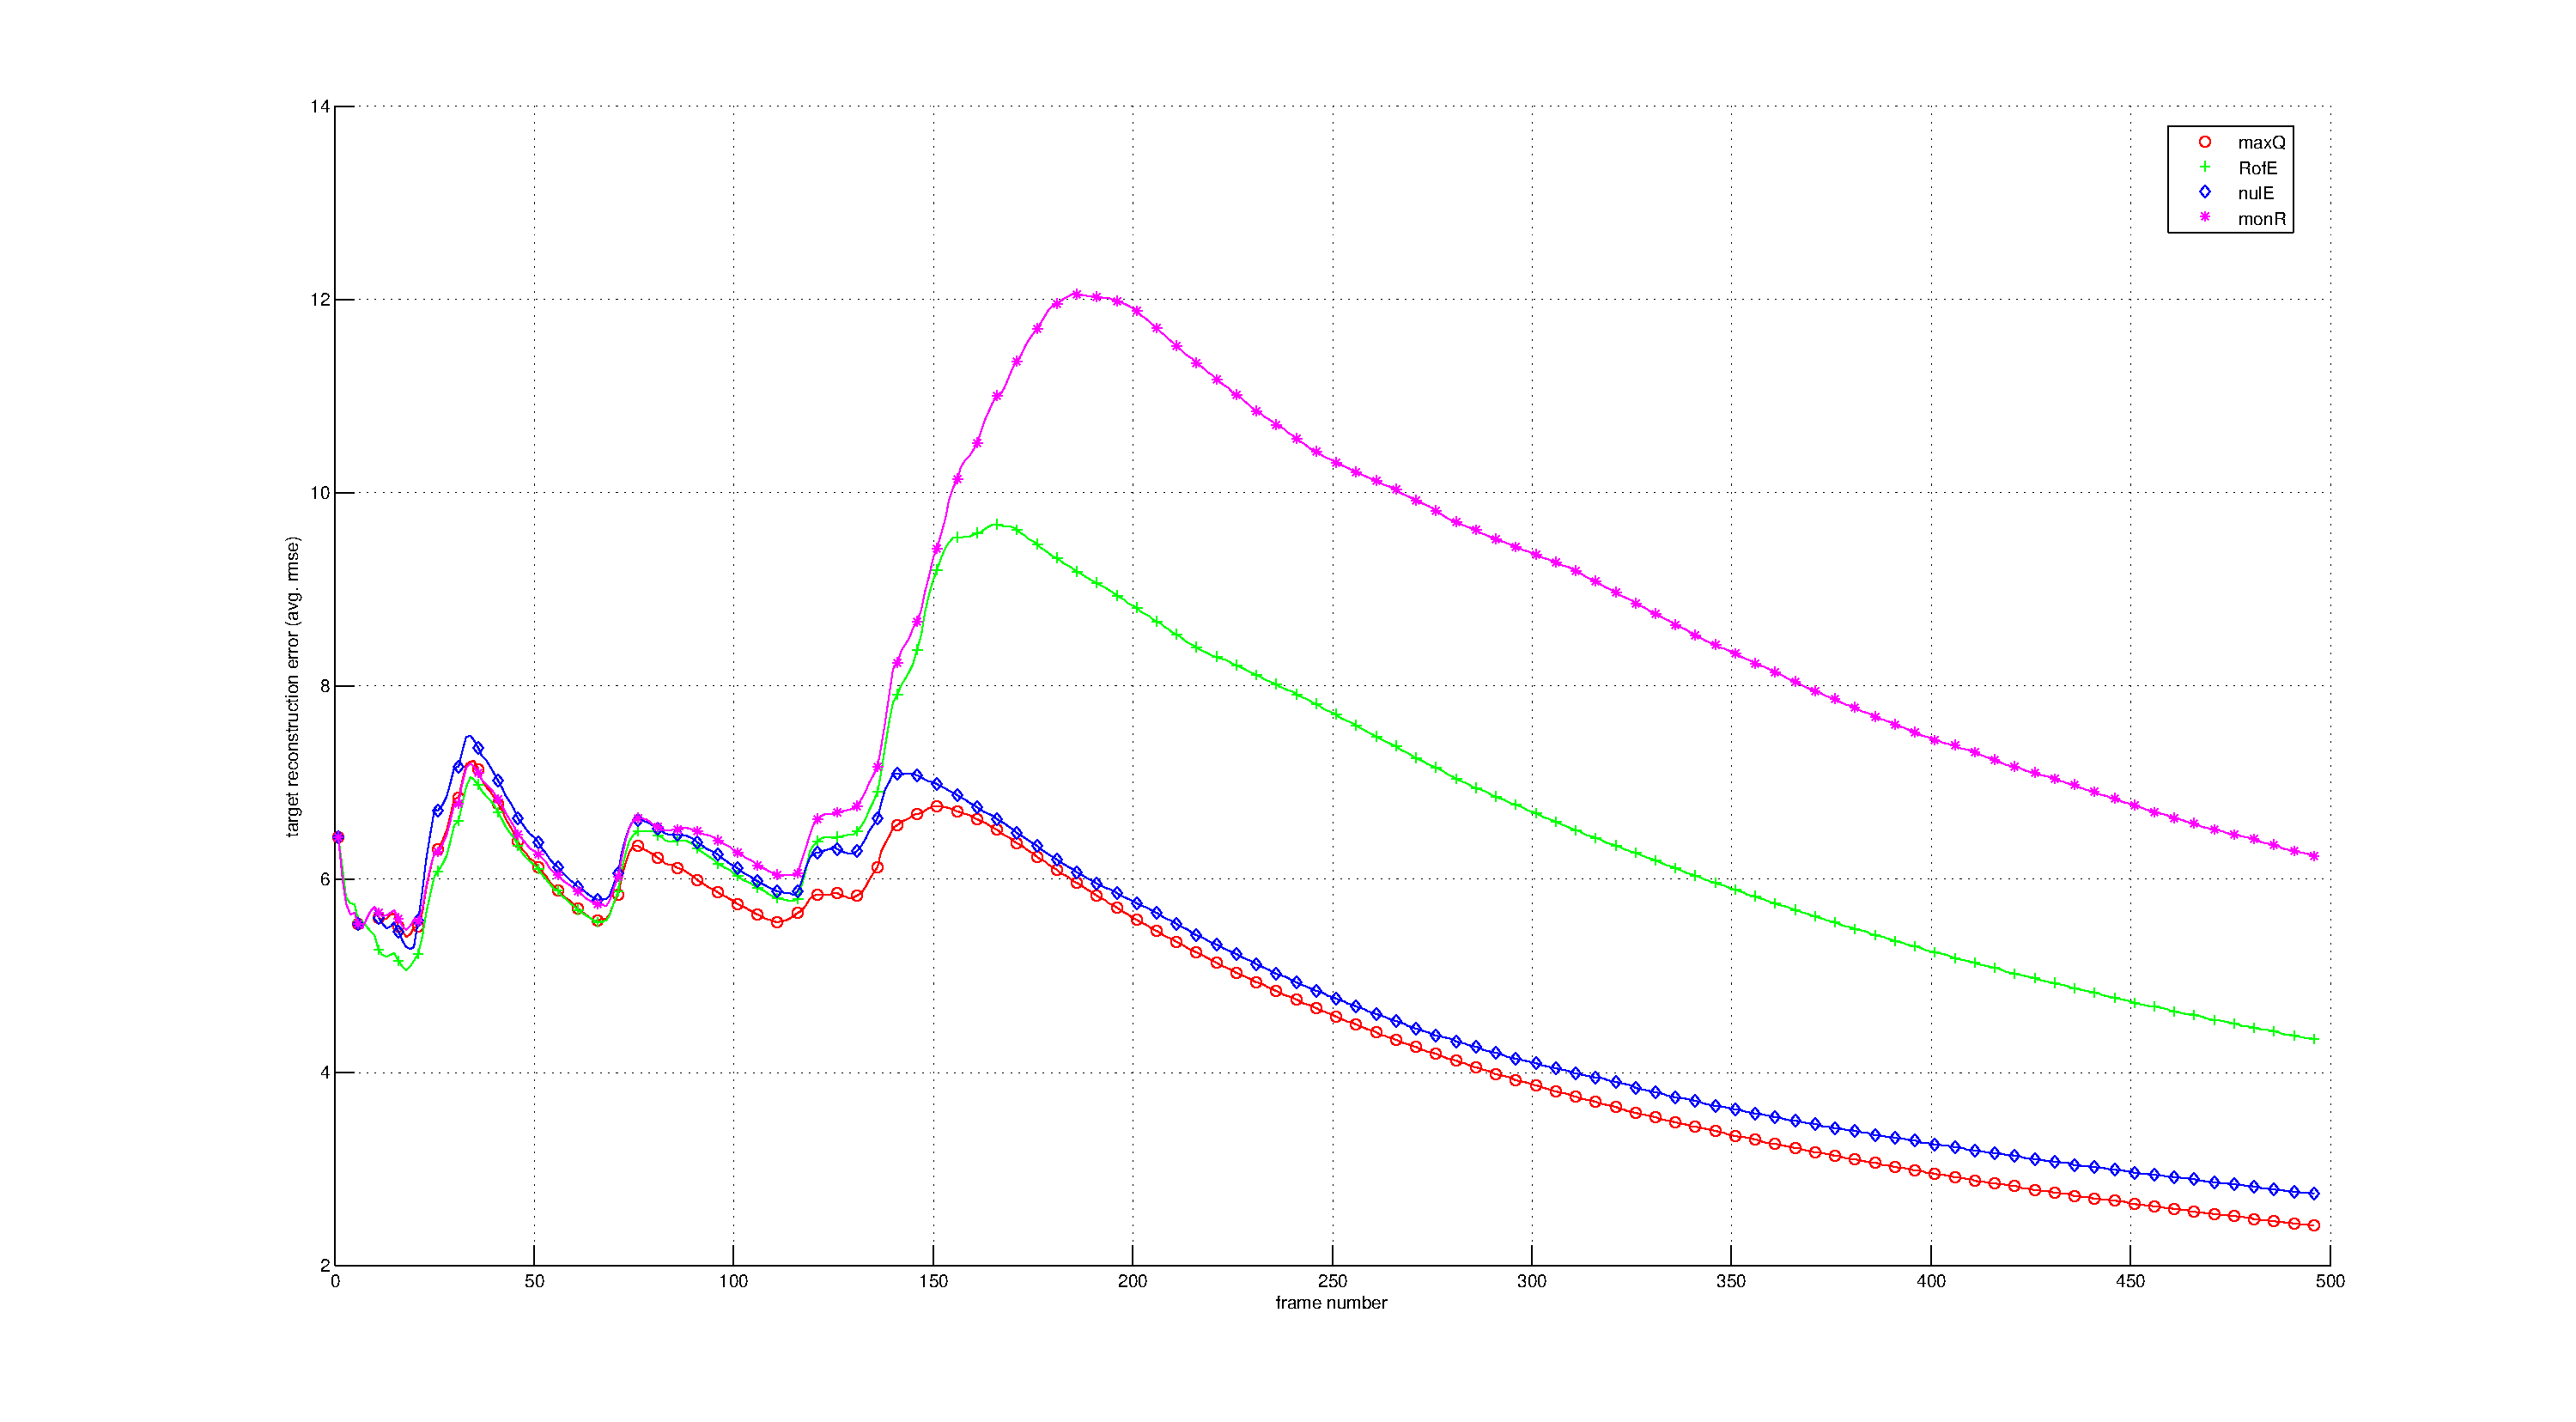
\includegraphics[height=0.4\textheight]{thesis/4_trellis70_8_4_1000_snp_armse.pdf}
								\caption{8x4 RVQ, snippet reconstruction error (avg. rmse).}
								\label{fig:4_trellis70_8_4_1000_snp_armse}
								\end{figure}

								\begin{figure}[h!]
								\centering
								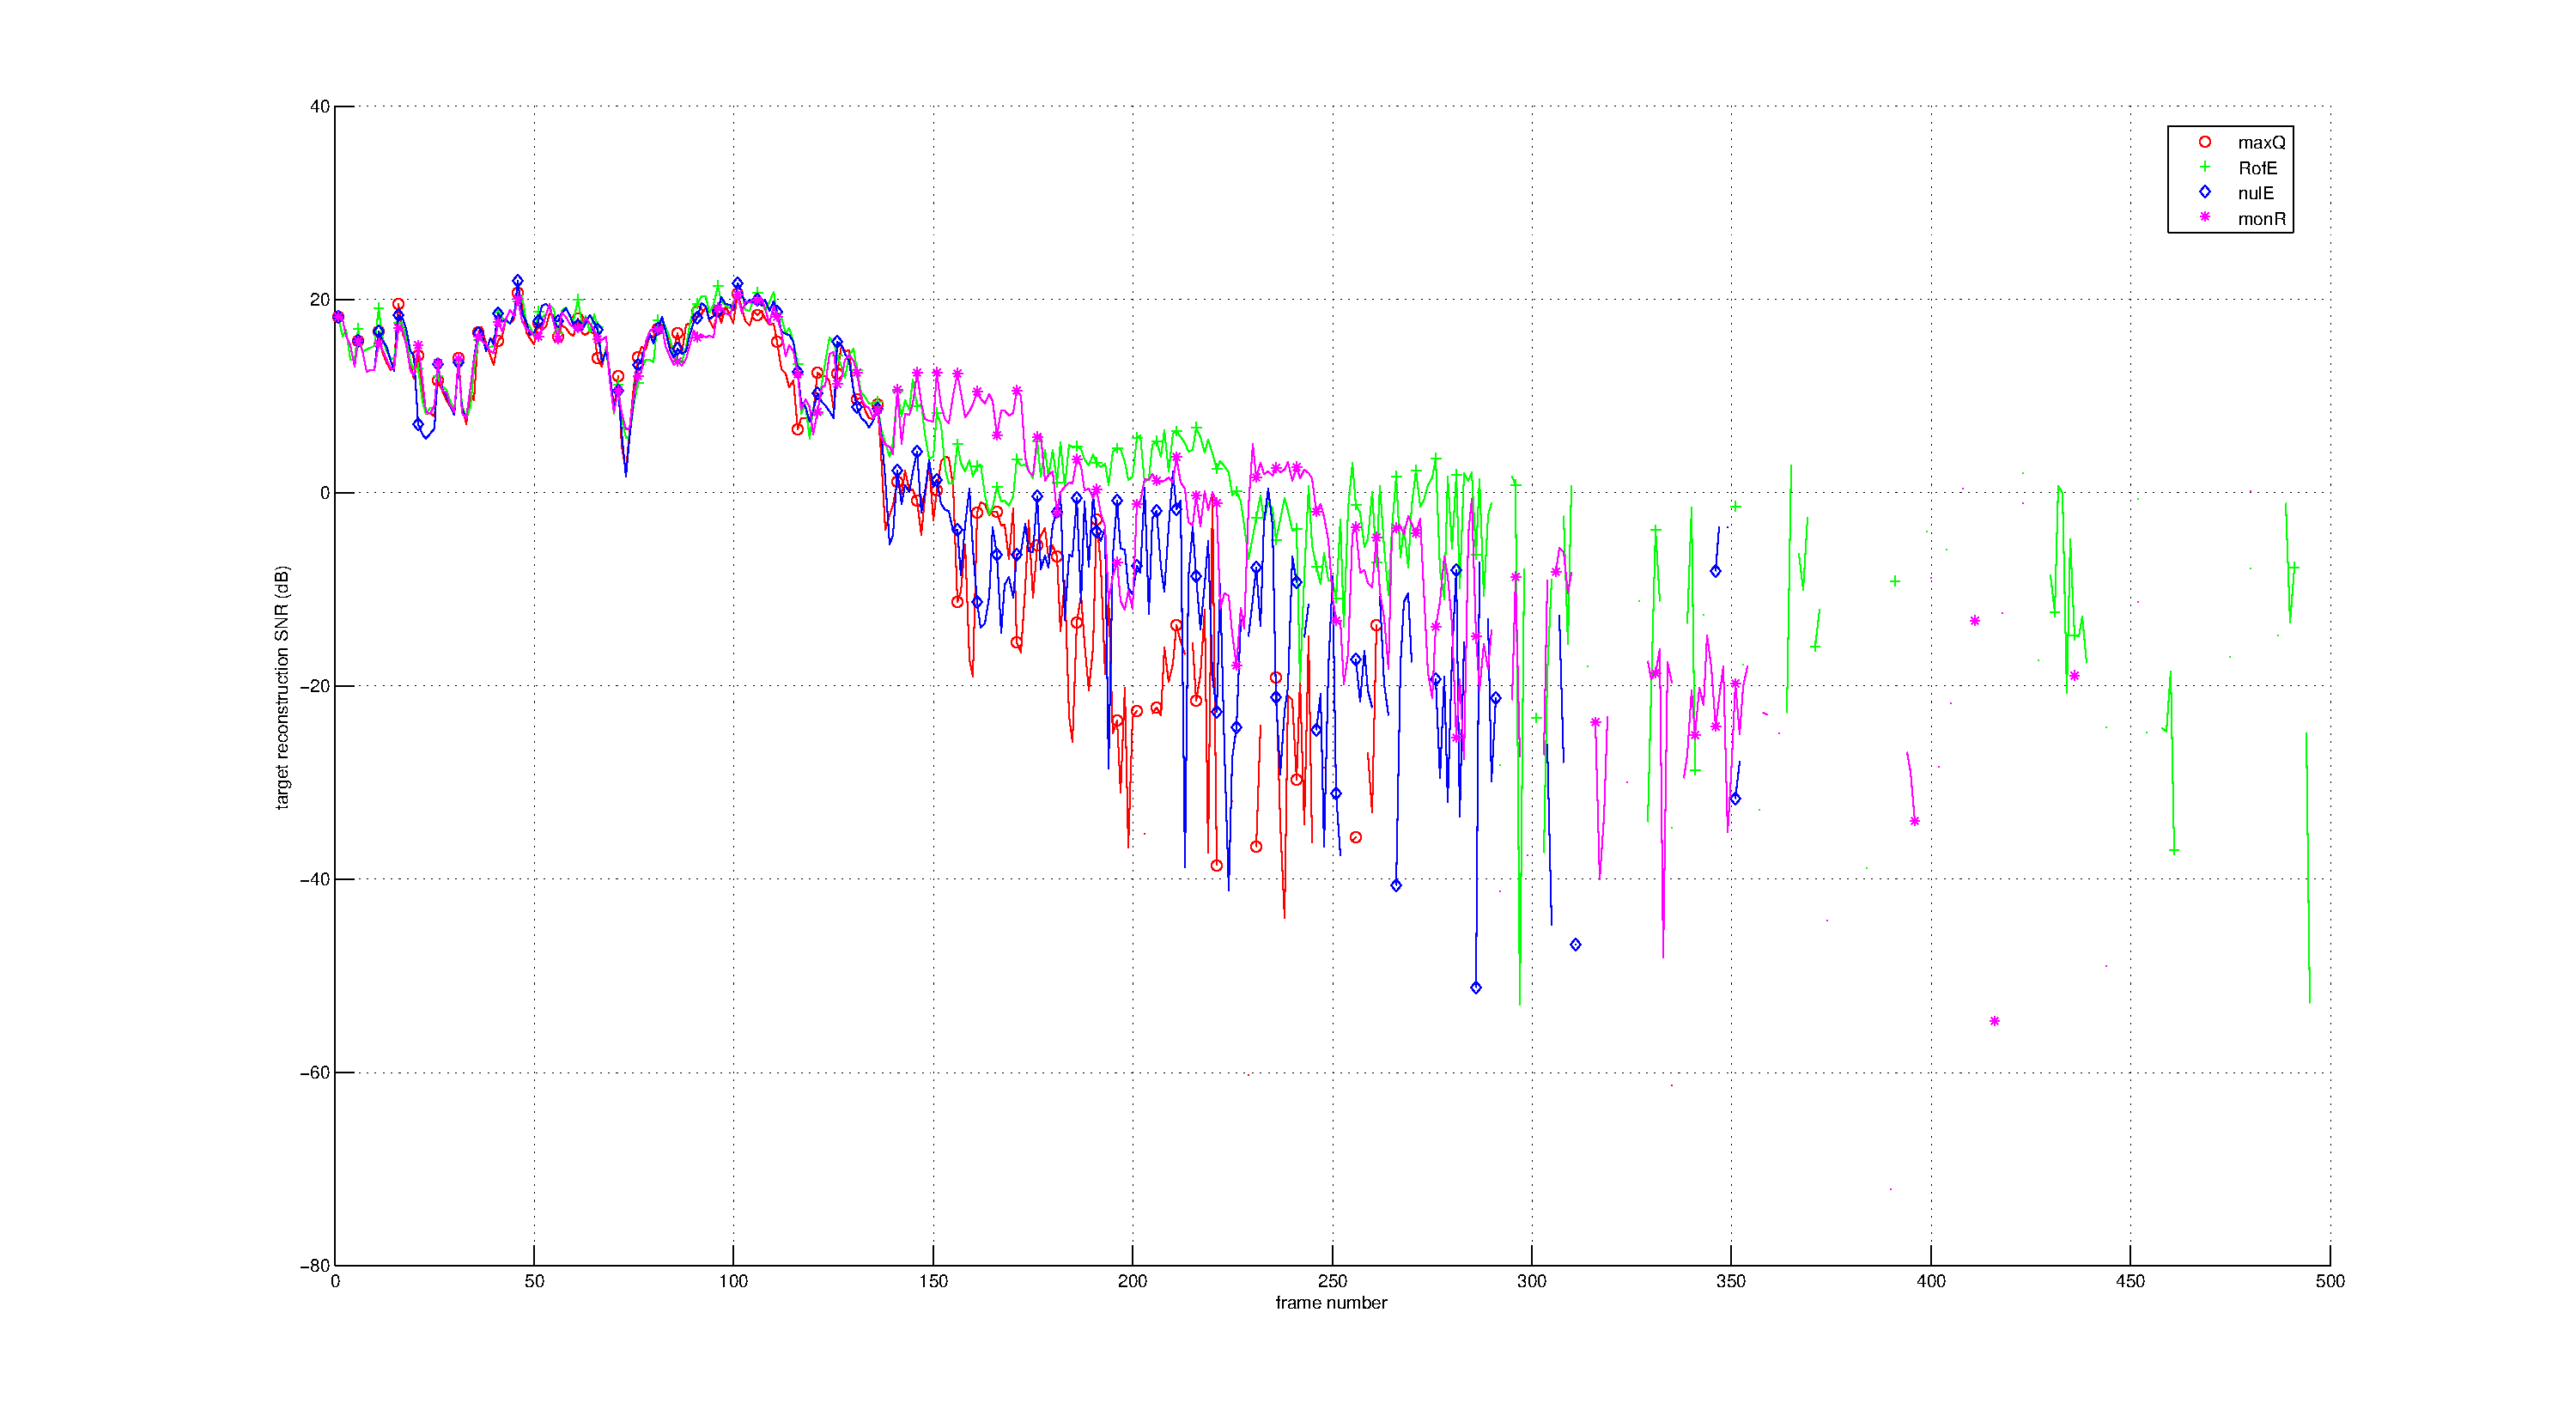
\includegraphics[height=0.4\textheight]{thesis/4_trellis70_8_4_1000_snp_SNRdB.pdf}
								\caption{8x4 RVQ, snippet reconstruction SNR in dB.}
								\label{fig:4_trellis70_8_4_1000_snp_SNRdB}
								\end{figure}
%------------------------------------
\clearpage
\newpage
\subsection{Learning}
%------------------------------------
								\begin{figure}[h!]
								\centering
								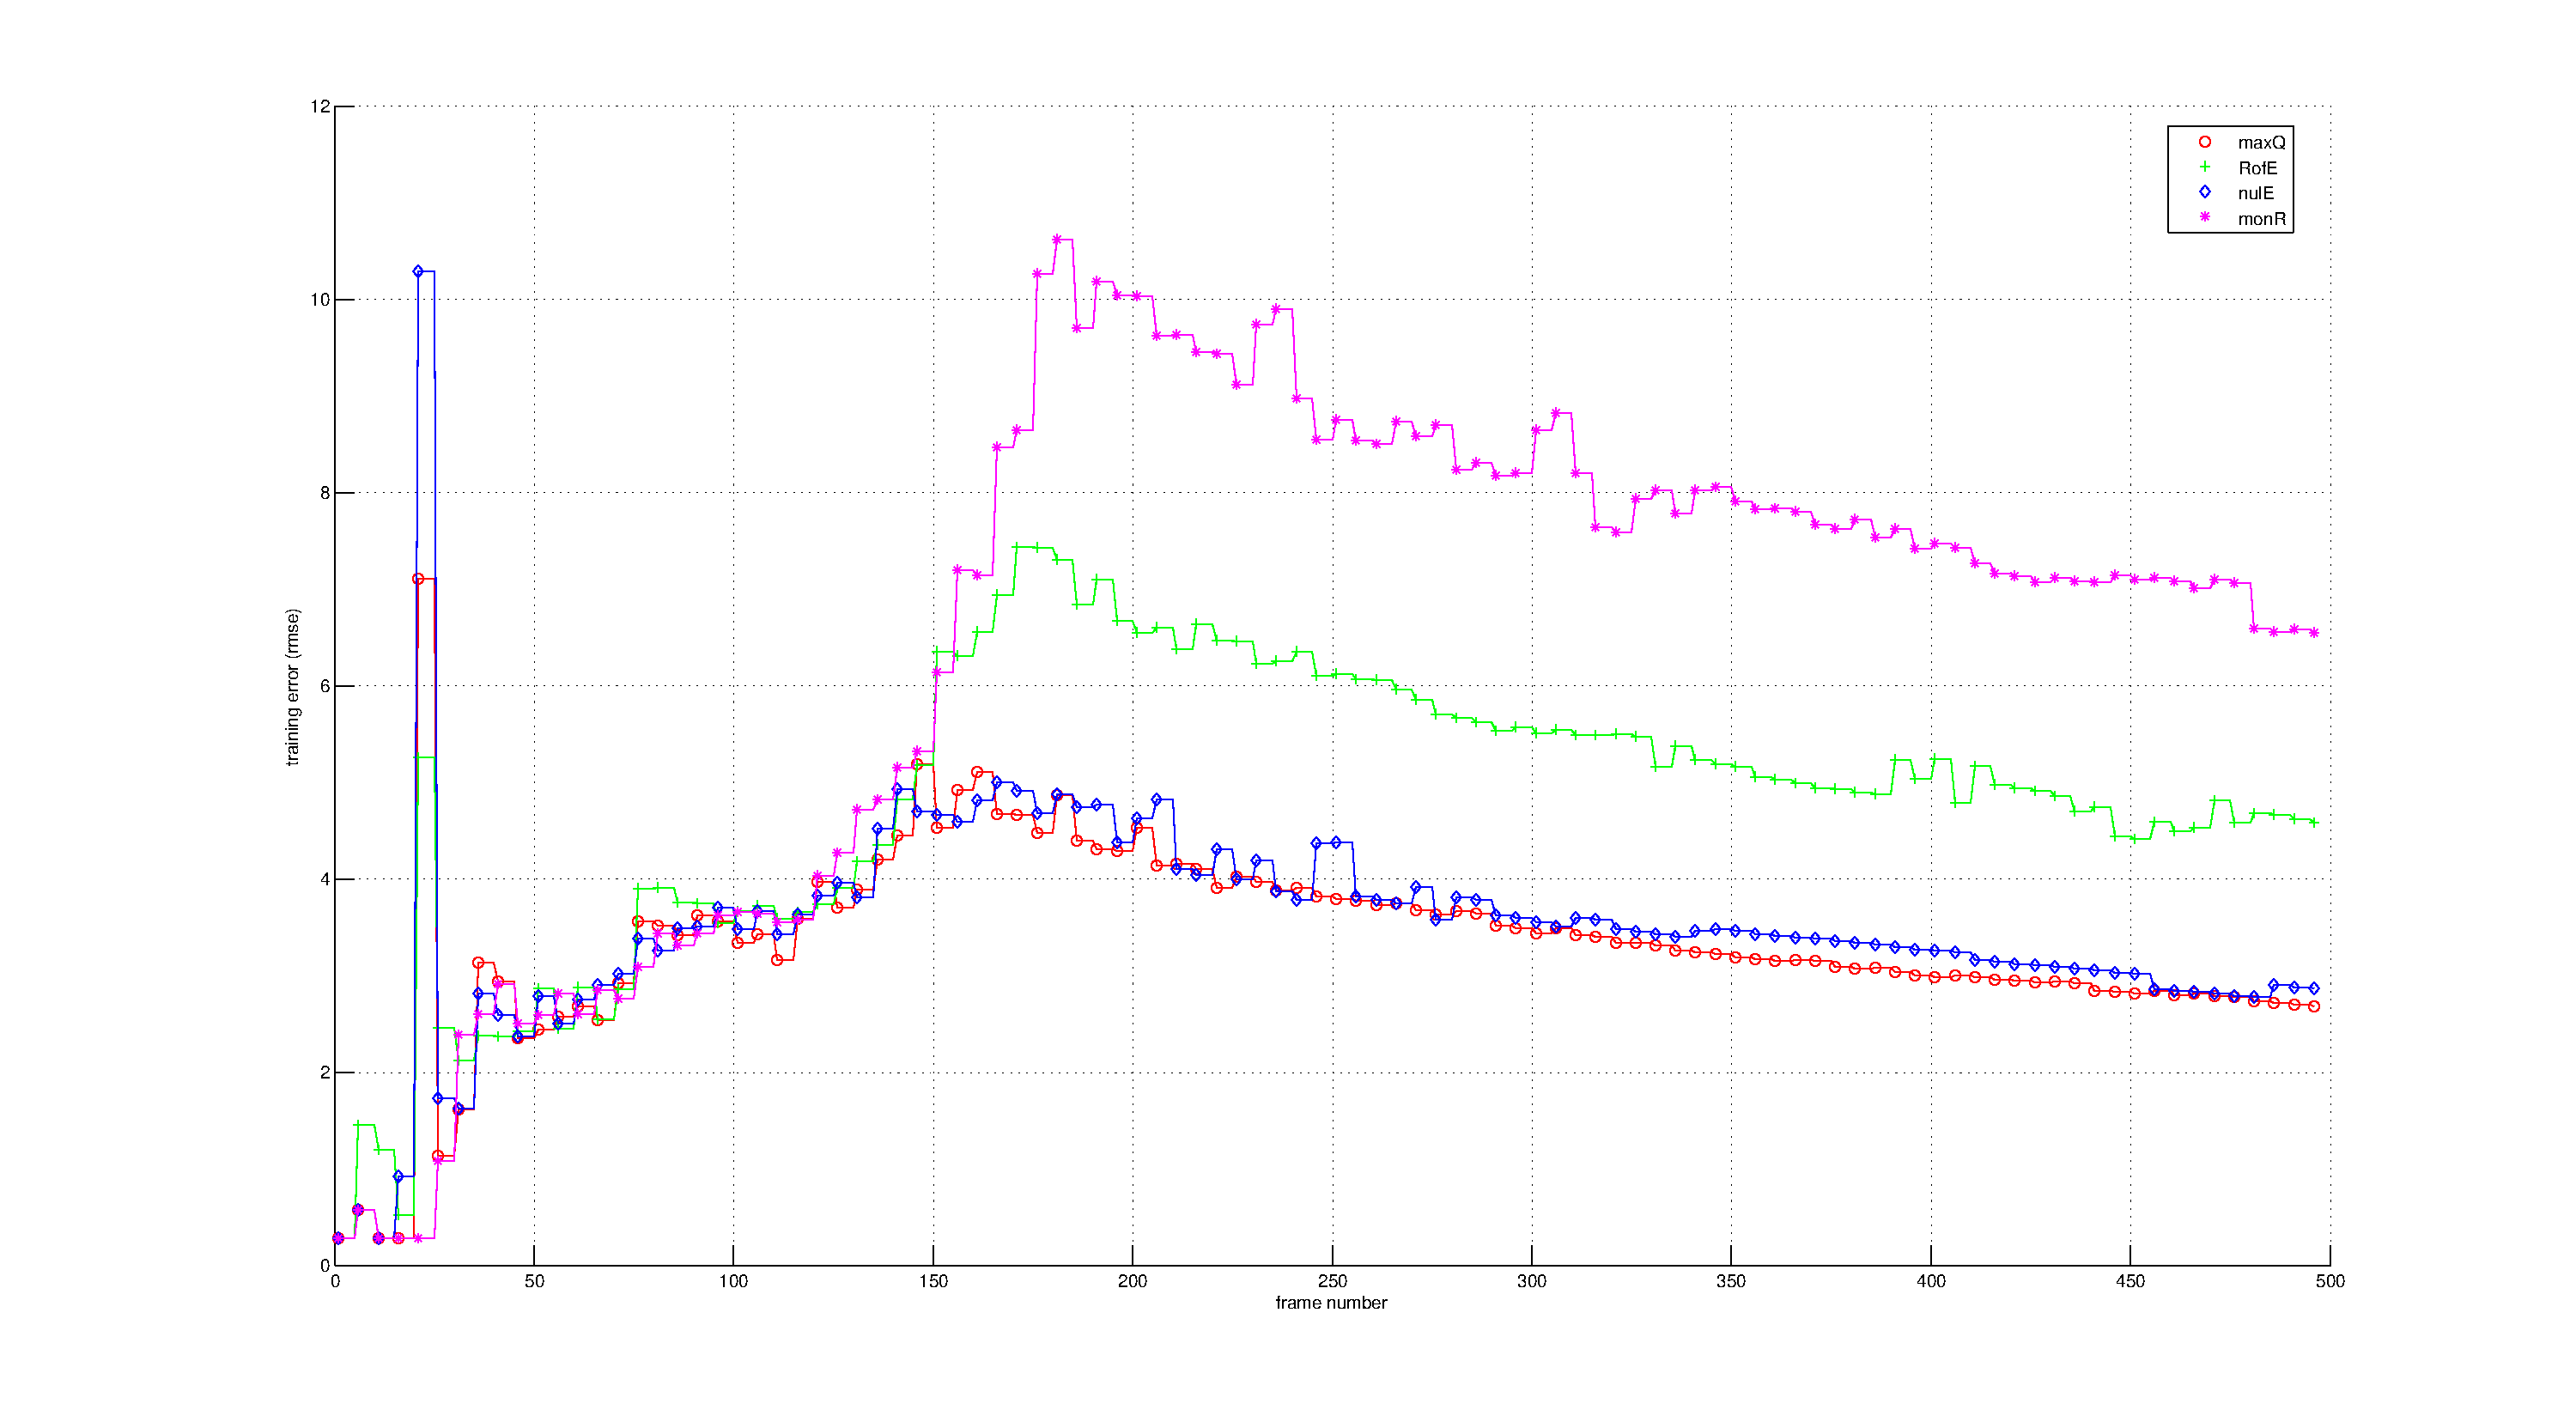
\includegraphics[height=0.4\textheight]{thesis/4_trellis70_8_4_1000_trg_rmse.pdf}
								\caption{8x4 RVQ, training error (rmse).}
								\label{fig:4_trellis70_8_4_1000_trg_rmse}
								\end{figure}


								\begin{figure}[h!]
								\centering
								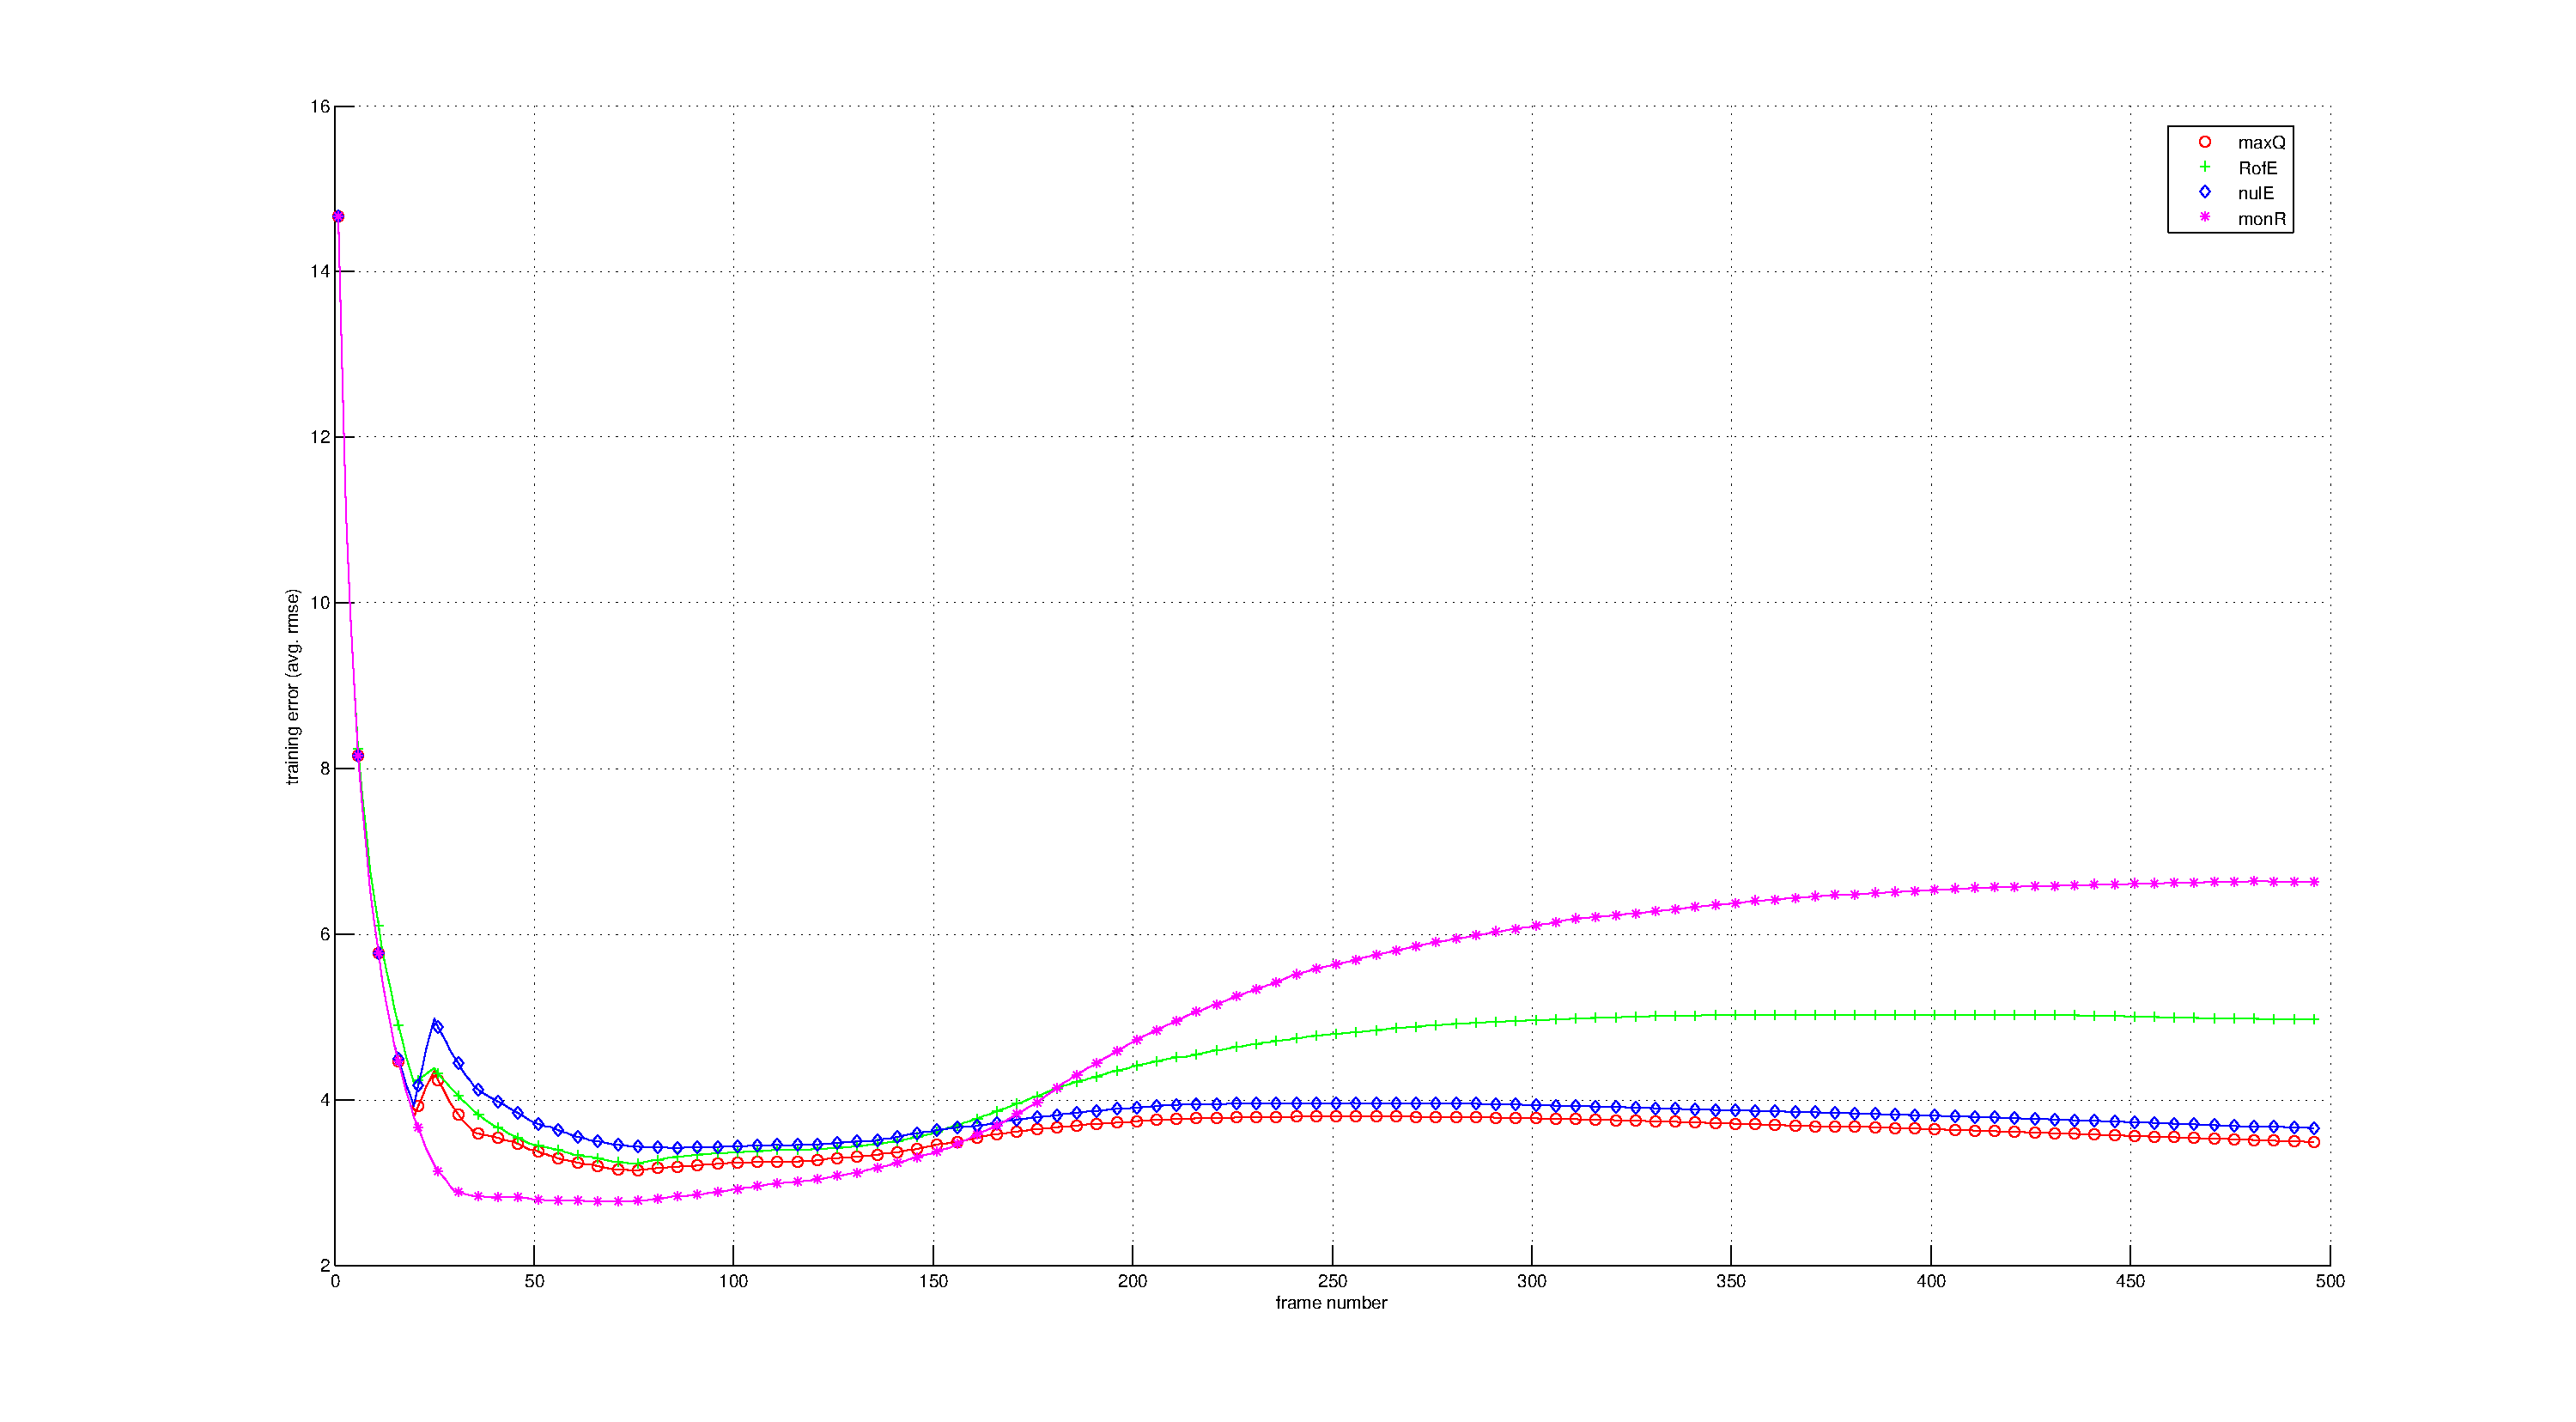
\includegraphics[height=0.4\textheight]{thesis/4_trellis70_8_4_1000_trg_armse.pdf}
								\caption{8x4 RVQ, training error (avg. rmse).}
								\label{fig:4_trellis70_8_4_1000_trg_armse}
								\end{figure}

								\begin{figure}[h!]
								\centering
								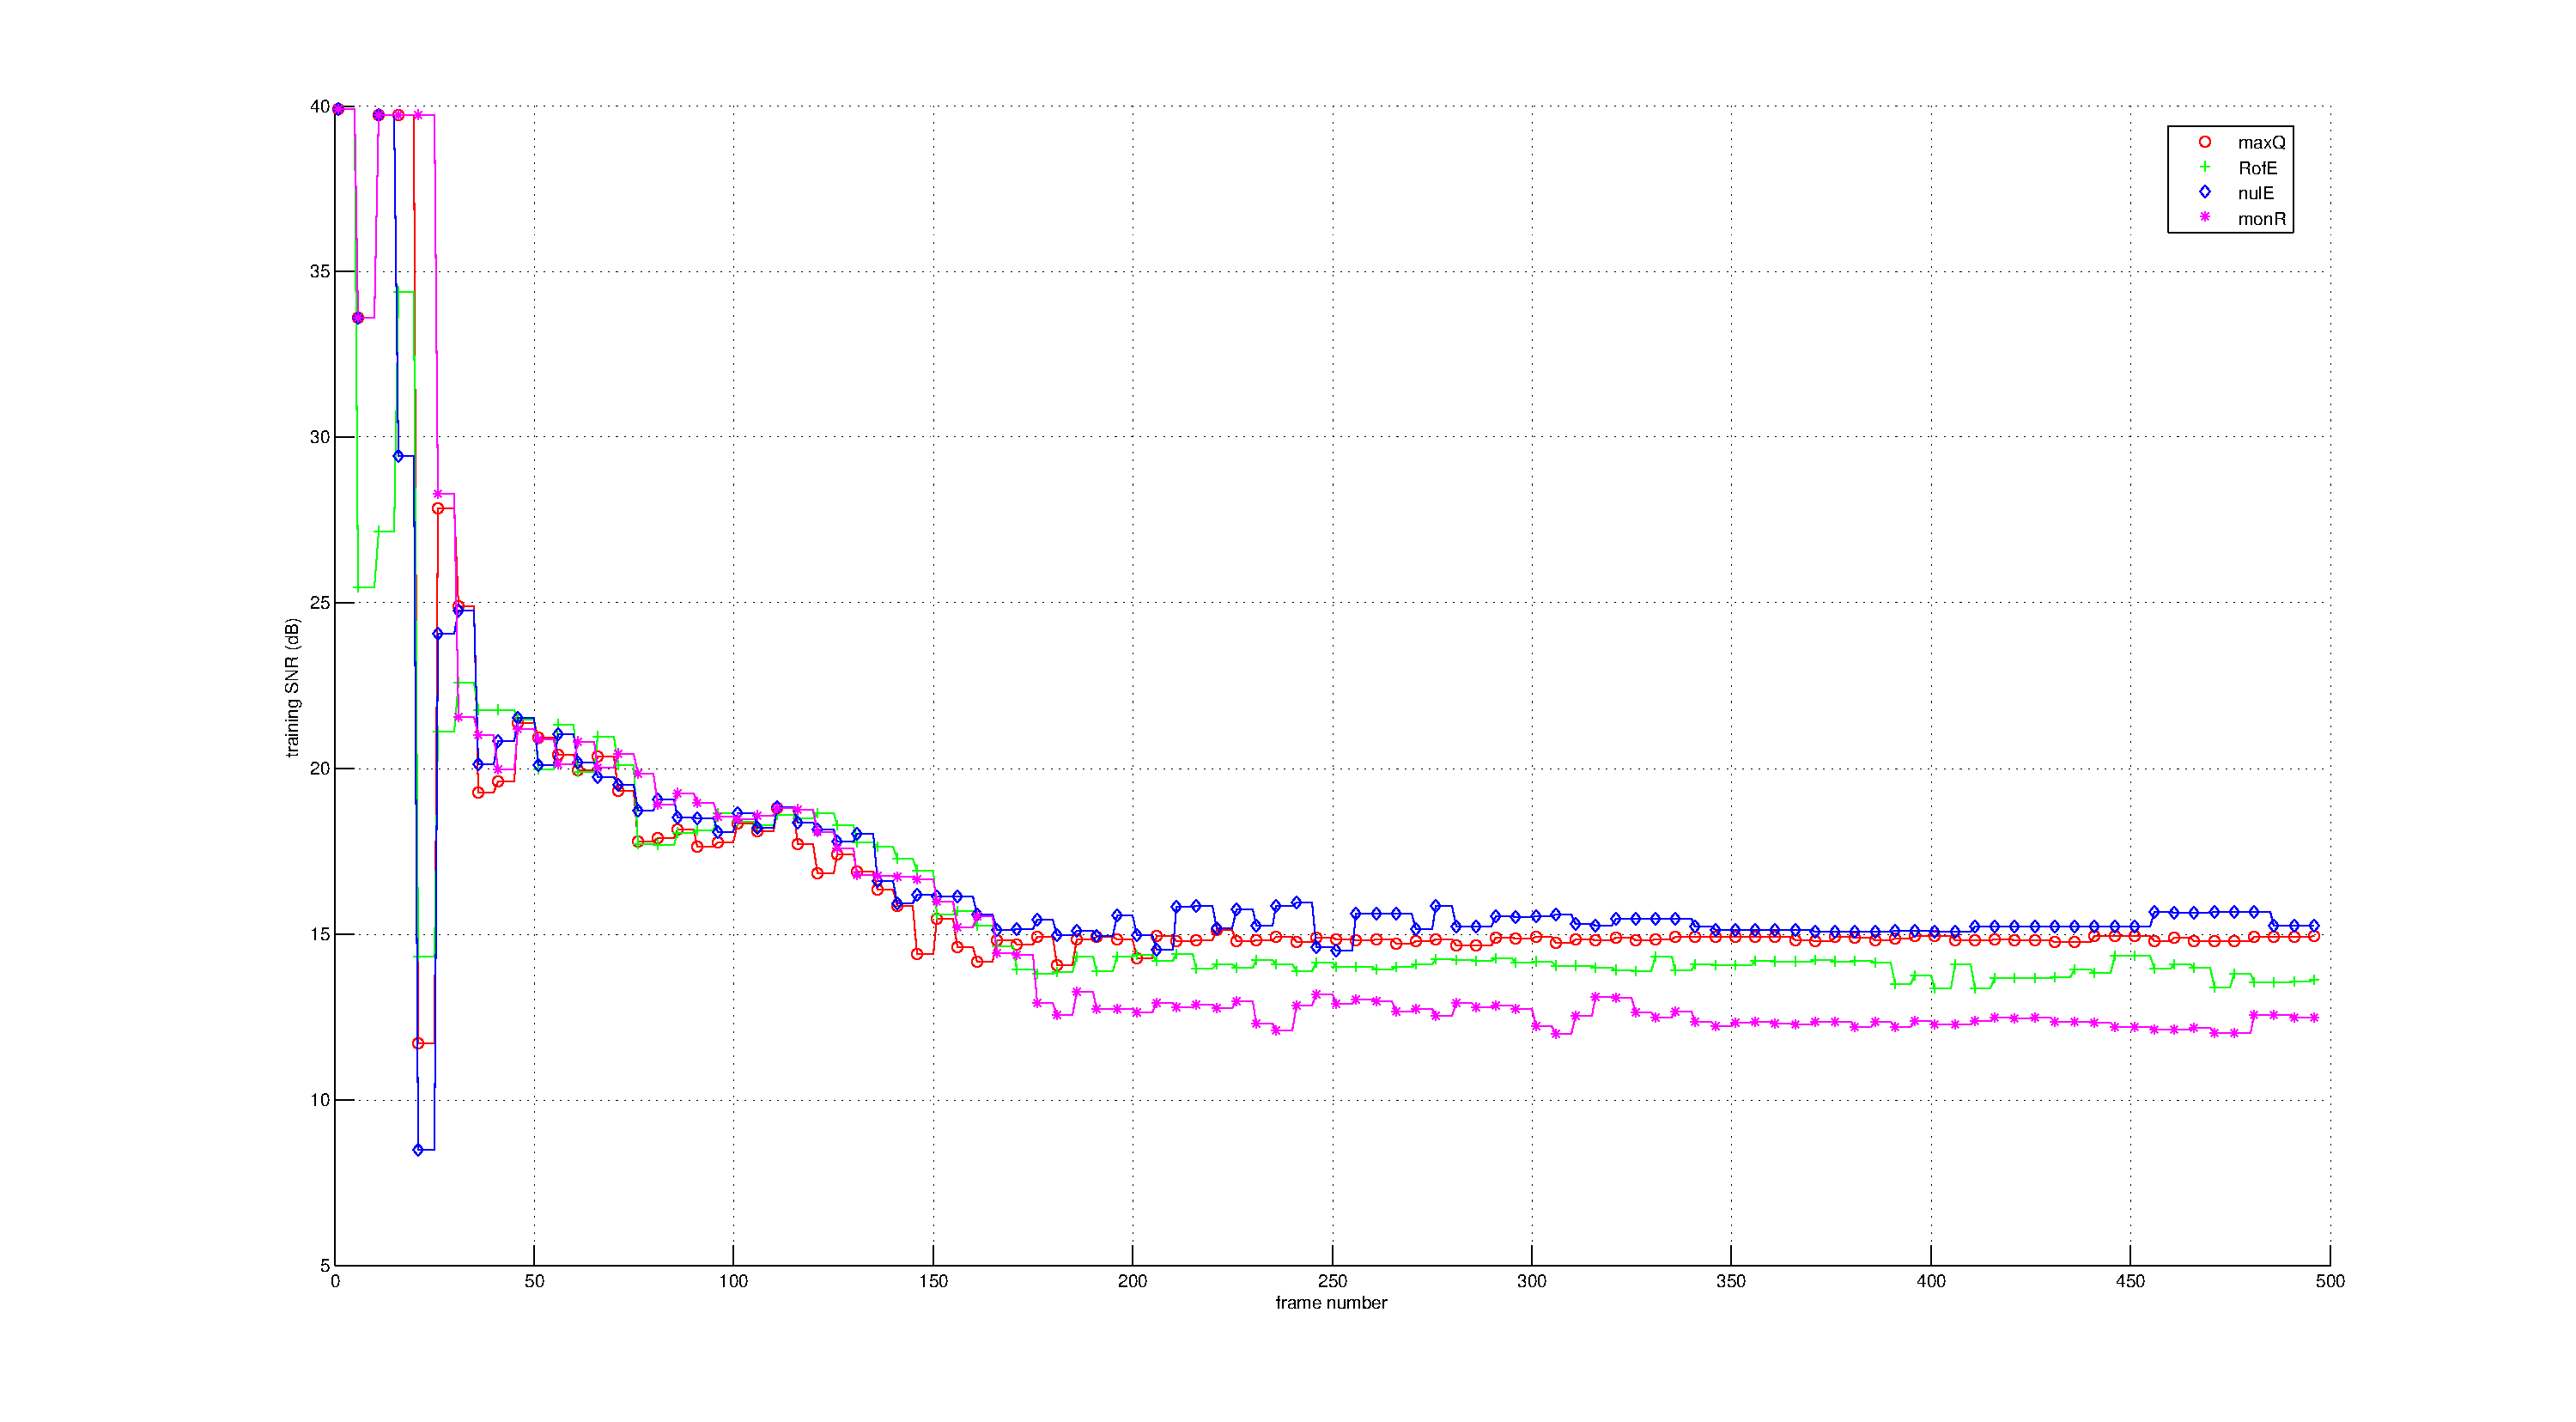
\includegraphics[height=0.4\textheight]{thesis/4_trellis70_8_4_1000_trg_SNRdB.pdf}
								\caption{8x4 RVQ, training SNR in dB.}
								\label{fig:4_trellis70_8_4_1000_trg_SNRdB}
								\end{figure}
%------------------------------------
\clearpage
\newpage
\subsection{Testing}
%------------------------------------
								\begin{figure}[h!]
								\centering
								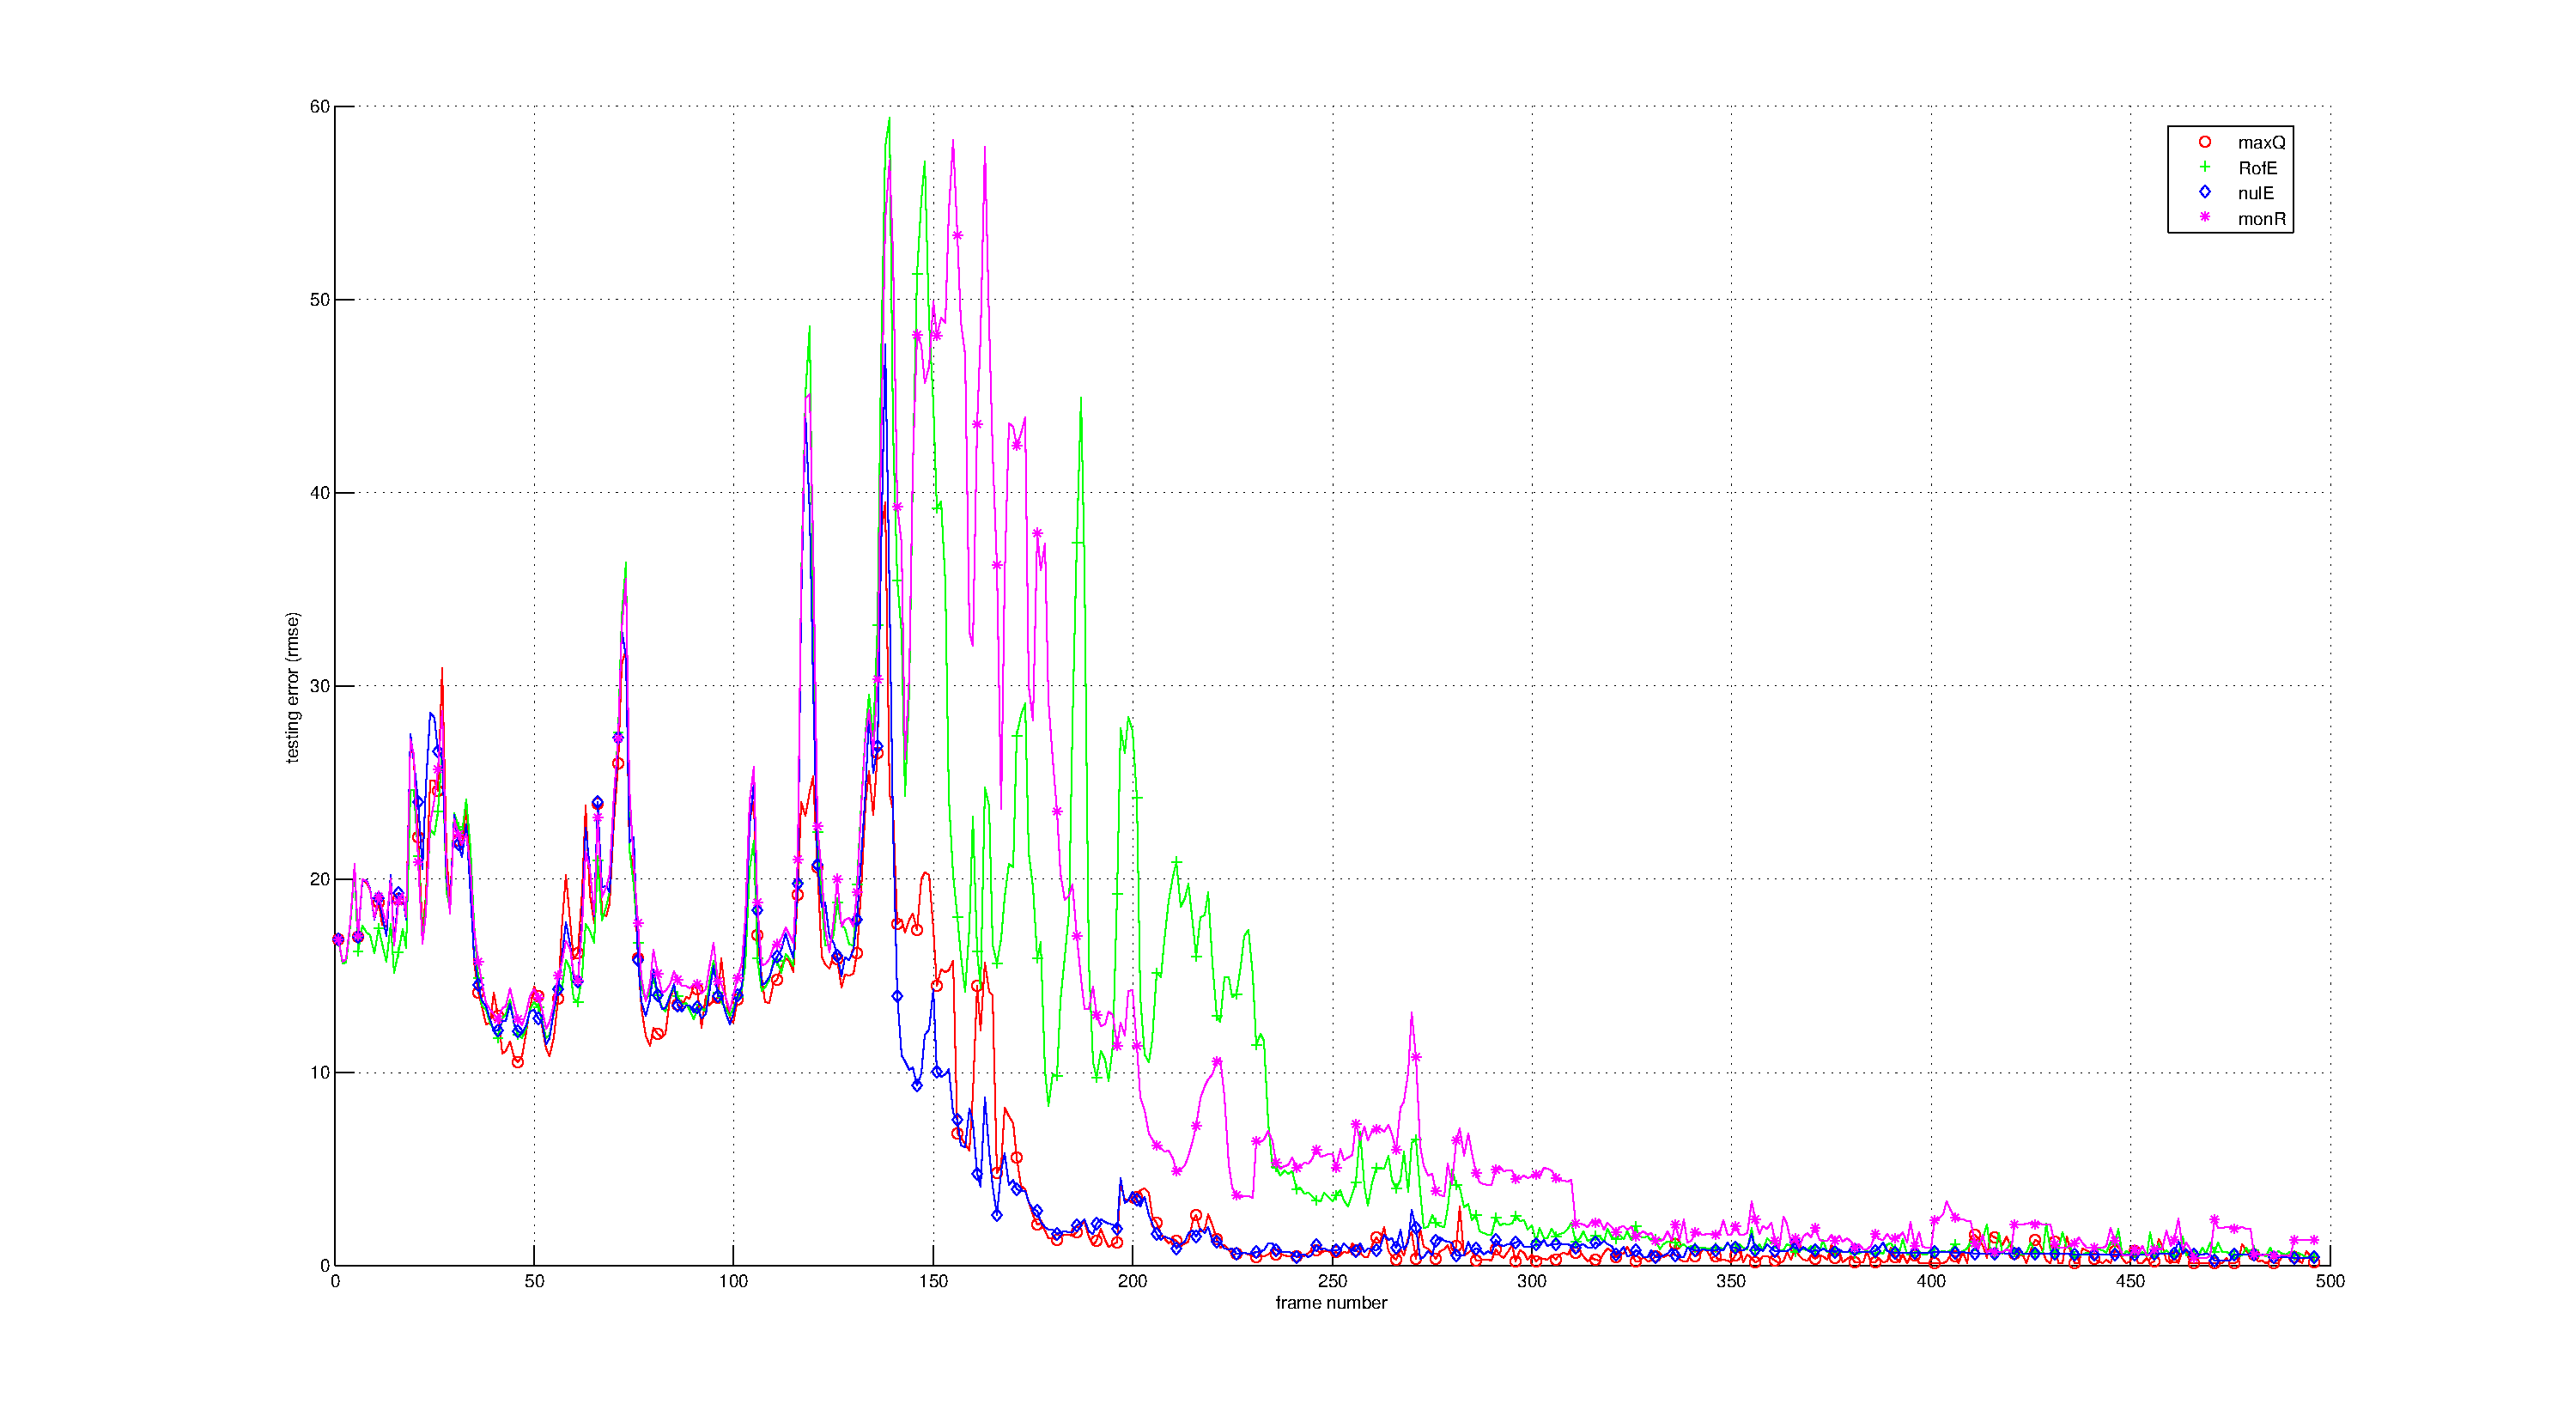
\includegraphics[height=0.4\textheight]{thesis/4_trellis70_8_4_1000_tst_rmse.pdf}
								\caption{8x4 RVQ, testing error (rmse).}
								\label{fig:4_trellis70_8_4_1000_tst_rmse}
								\end{figure}


								\begin{figure}[h!]
								\centering
								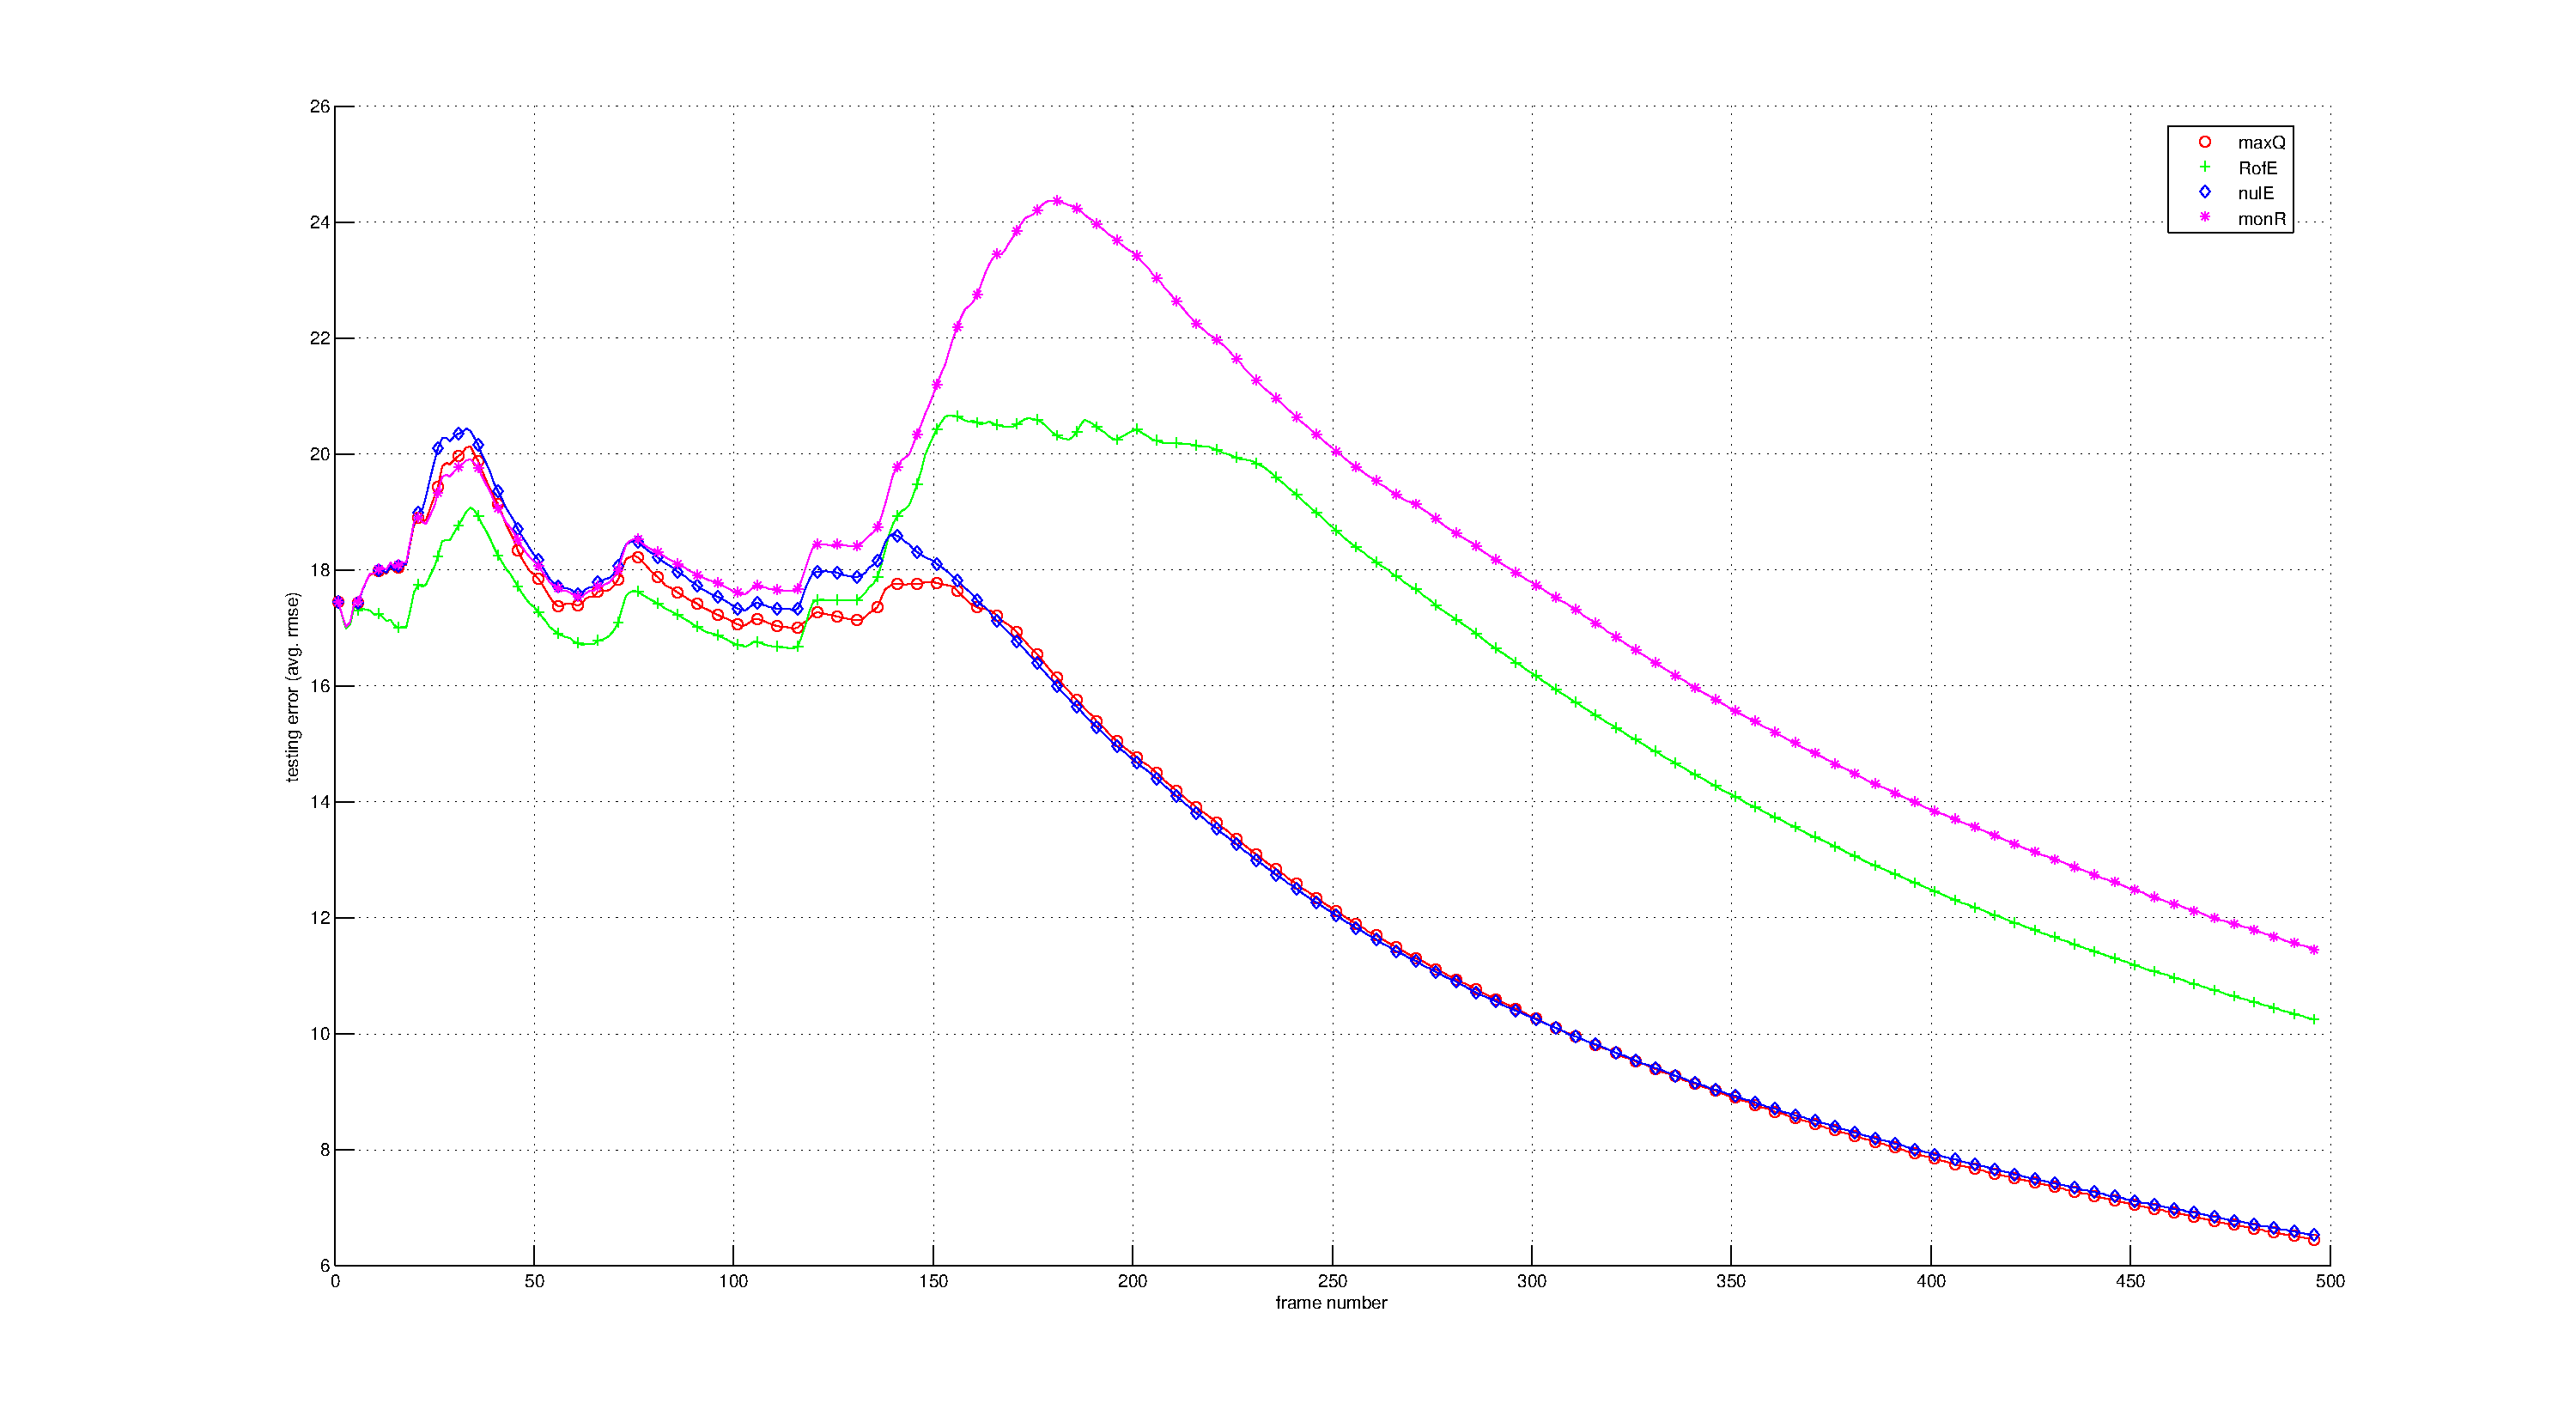
\includegraphics[height=0.4\textheight]{thesis/4_trellis70_8_4_1000_tst_armse.pdf}
								\caption{8x4 RVQ, testing error (avg. rmse).}
								\label{fig:4_trellis70_8_4_1000_tst_armse}
								\end{figure}

								\begin{figure}[h!]
								\centering
								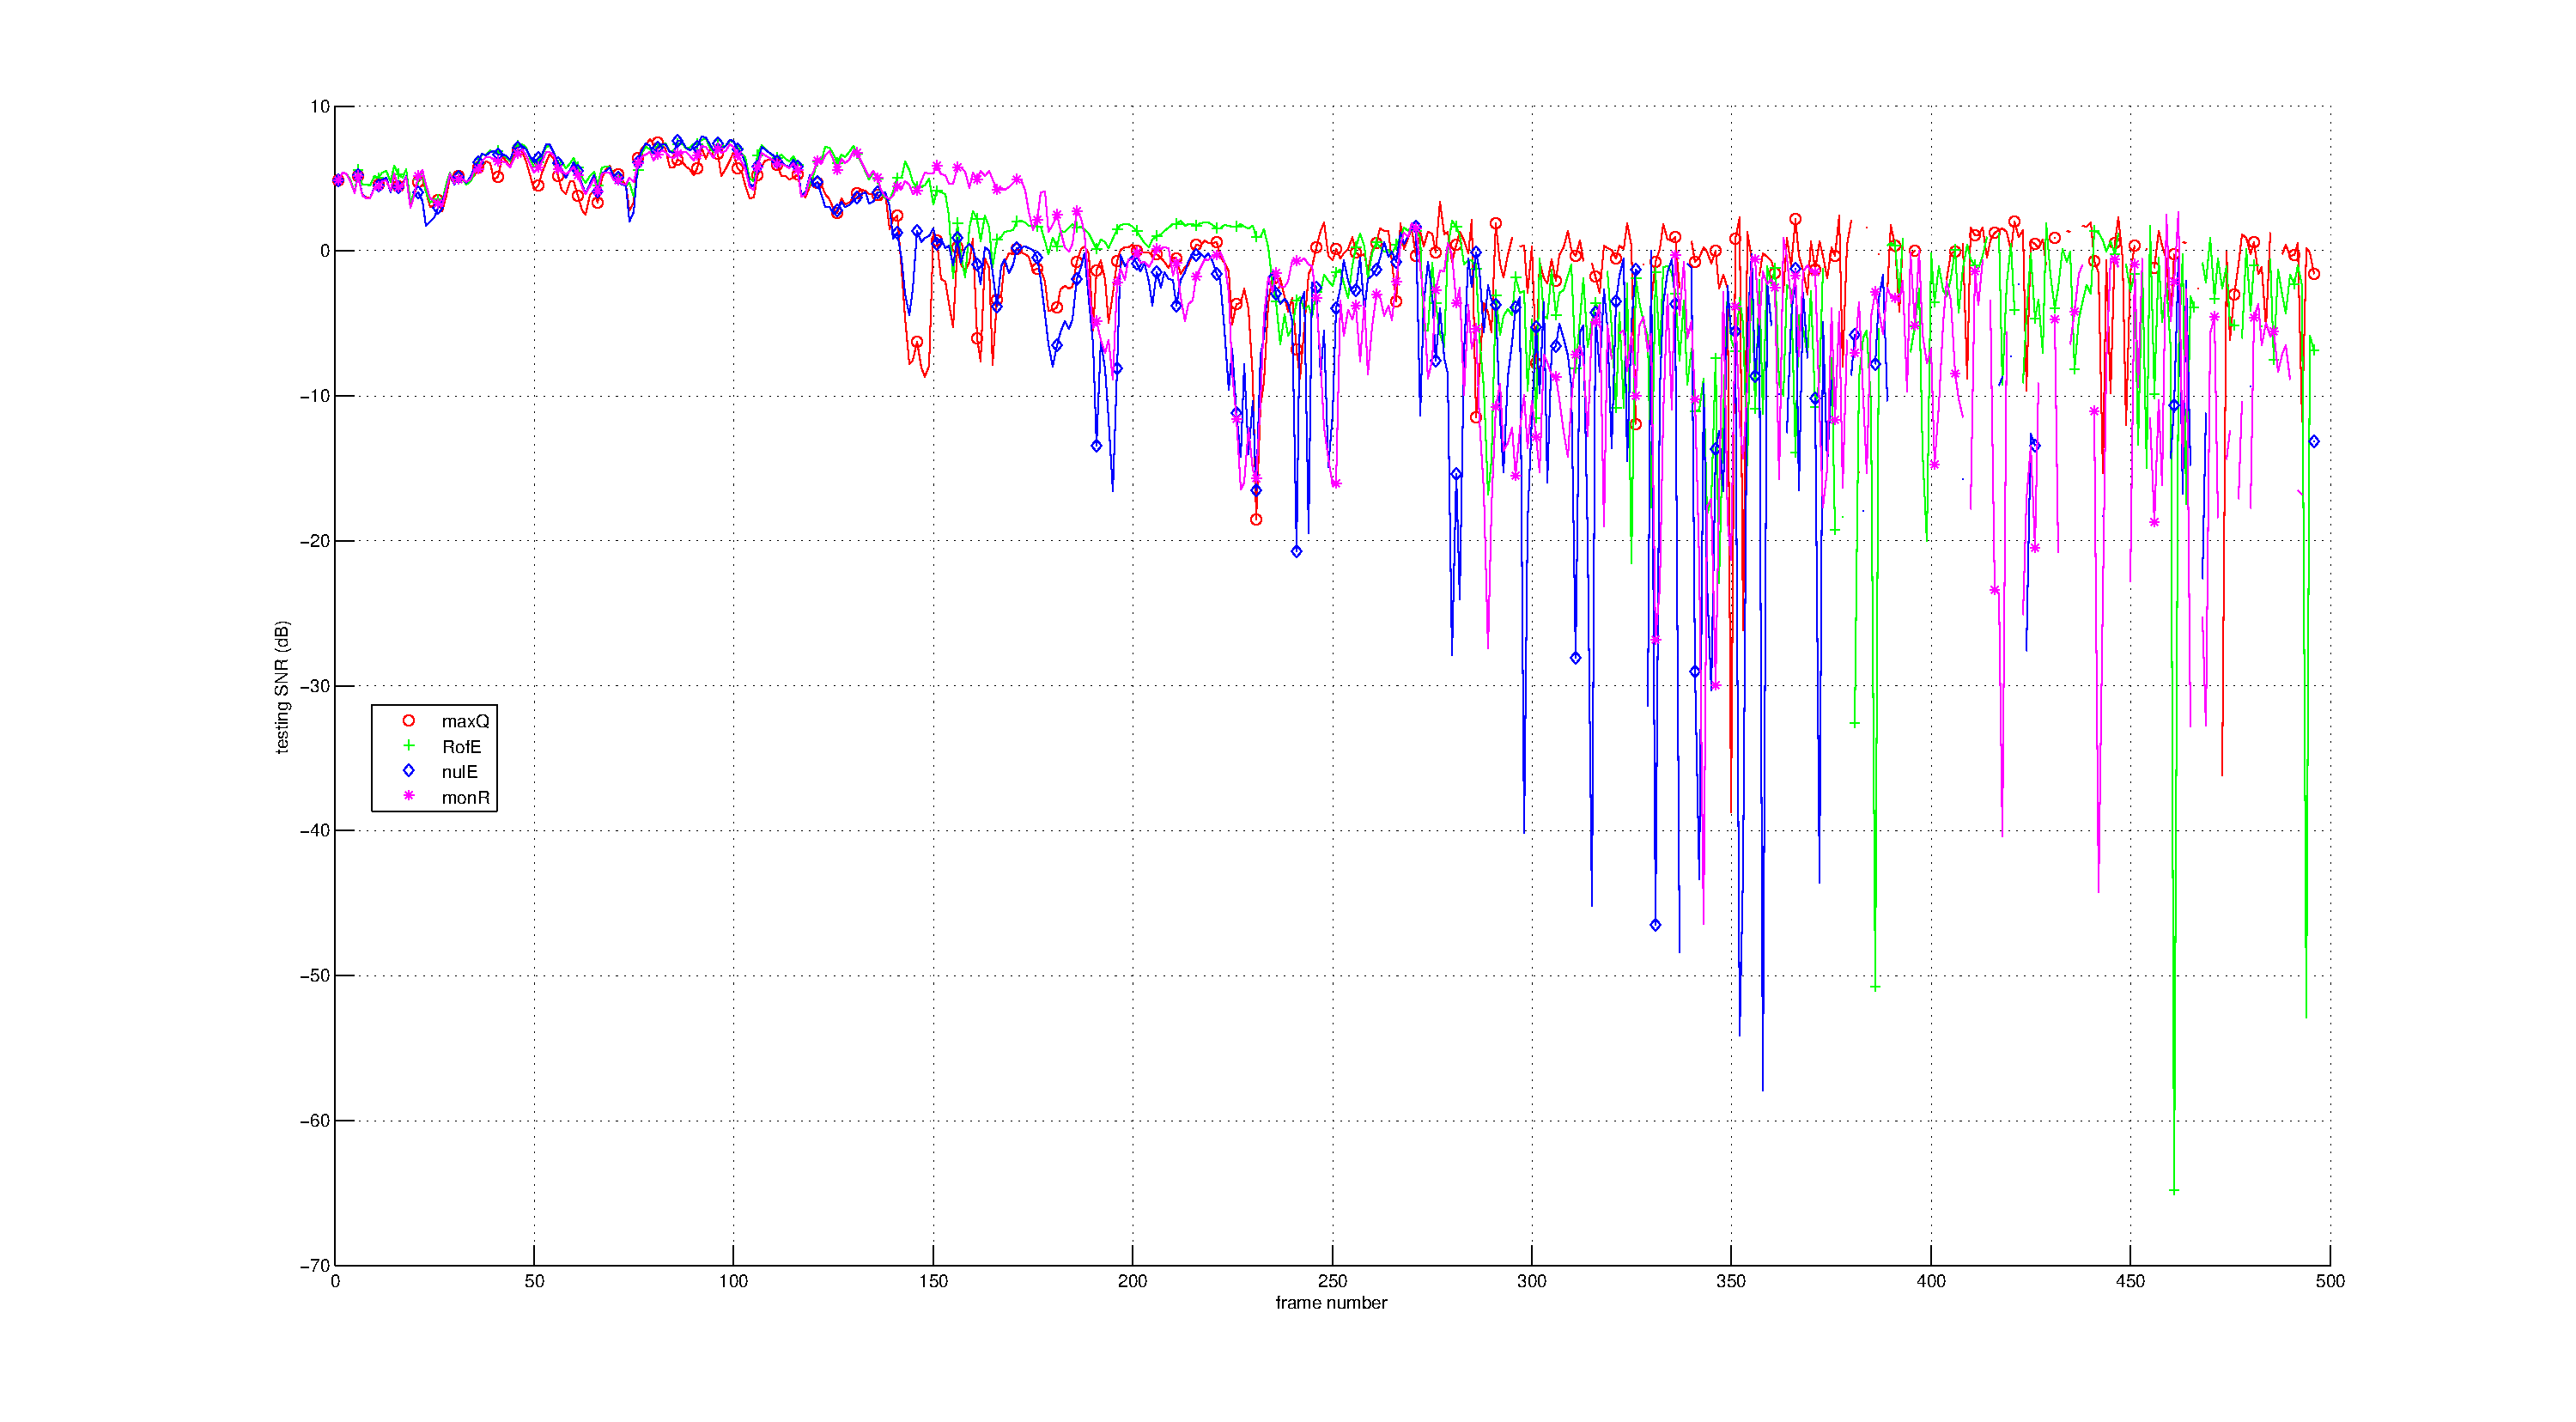
\includegraphics[height=0.4\textheight]{thesis/4_trellis70_8_4_1000_tst_SNRdB.pdf}
								\caption{8x4 RVQ,testing SNR in dB.}
								\label{fig:4_trellis70_8_4_1000_tst_SNRdB}
								\end{figure}
%%===============================
\clearpage
\newpage
\section{Tracking: Fish dataset} 
%===============================
								\begin{figure}[h!]
								\centering
								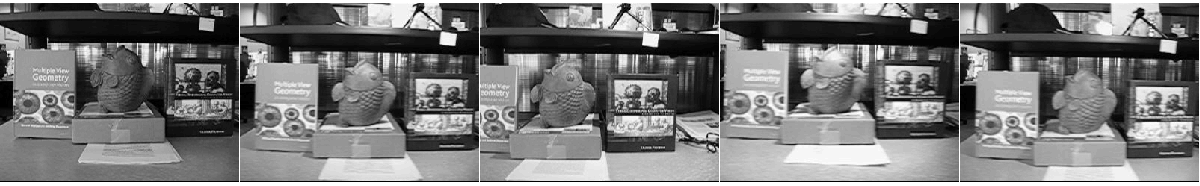
\includegraphics[width=1.0\textwidth]{figs/seq_5_fish.png}
								\caption{Fish dataset.}
								\label{fig:seq_5_fish}
								\end{figure}



\begin{table}[h]
\centering
\begin{tabular}{|l|c|c|c|c|}
\hline
&\textbf{maxQ}&\textbf{RofE}&\textbf{nulE}&\textbf{monR}\\\hline
\textbf{2}&2.73&3.82&3.93&3.32\\\hline
\textbf{4}&2.84&2.97&10.40&2.60\\\hline
\textbf{8}&13.09&2.60&13.97&13.29\\\hline
\textbf{12}&5.24&5.37&4.52&4.44\\\hline
\textbf{16}&4.42&12.04&4.87&4.37\\\hline
\end{tabular}

\caption{Tracking errors for various RVQ configurations.  -1 means that track was lost.  These results show that RVQ is able to track the object of interest very closely.}
\end{table}

For the interested reader, detailed graphical results follow for 8x4 RVQ.
%------------------------------------
\clearpage
\newpage
\subsection{Tracking error}
%------------------------------------

								\begin{figure}[h!]
								\centering
								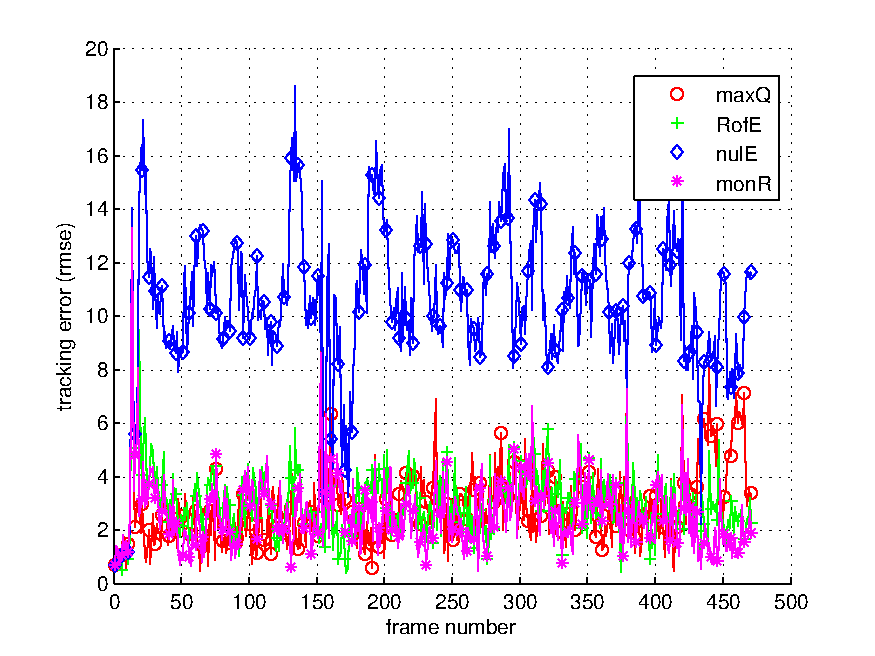
\includegraphics[height=0.38\textheight]{figs/5_fish_8_4_1000_trk_rmse.pdf}
								\caption{8x4 RVQ, tracking error (rmse).}
								\label{fig:5_fish_8_4_1000_trk_rmse}
								\end{figure}


								\begin{figure}[h!]
								\centering
								\includegraphics[height=0.38\textheight]{figs/5_fish_8_4_1000_trk_armse.pdf}
								\caption{8x4 RVQ, tracking error (average rmse).}
								\label{fig:5_fish_8_4_1000_trk_avg_rmse}
								\end{figure}

%------------------------------------
\clearpage
\newpage
\subsection{Target reconstruction}
%------------------------------------

								\begin{figure}[h!]
								\centering
								\includegraphics[height=0.4\textheight]{figs/5_fish_8_4_1000_snp_rmse.pdf}
								\caption{8x4 RVQ, snippet reconstruction error (rmse).}
								\label{fig:5_fish_8_4_1000_snp_rmse}
								\end{figure}


								\begin{figure}[h!]
								\centering
								\includegraphics[height=0.4\textheight]{figs/5_fish_8_4_1000_snp_armse.pdf}
								\caption{8x4 RVQ, snippet reconstruction error (avg. rmse).}
								\label{fig:5_fish_8_4_1000_snp_armse}
								\end{figure}

								\begin{figure}[h!]
								\centering
								\includegraphics[height=0.4\textheight]{figs/5_fish_8_4_1000_snp_SNRdB.pdf}
								\caption{8x4 RVQ, snippet reconstruction SNR in dB.}
								\label{fig:5_fish_8_4_1000_snp_SNRdB}
								\end{figure}
%------------------------------------
\clearpage
\newpage
\subsection{Learning}
%------------------------------------

								\begin{figure}[h!]
								\centering
								\includegraphics[height=0.4\textheight]{figs/5_fish_8_4_1000_trg_rmse.pdf}
								\caption{8x4 RVQ, training error (rmse).}
								\label{fig:5_fish_8_4_1000_trg_rmse}
								\end{figure}


								\begin{figure}[h!]
								\centering
								\includegraphics[height=0.4\textheight]{figs/5_fish_8_4_1000_trg_armse.pdf}
								\caption{8x4 RVQ, training error (avg. rmse).}
								\label{fig:5_fish_8_4_1000_trg_armse}
								\end{figure}

								\begin{figure}[h!]
								\centering
								\includegraphics[height=0.4\textheight]{figs/5_fish_8_4_1000_trg_SNRdB.pdf}
								\caption{8x4 RVQ, training SNR in dB.}
								\label{fig:5_fish_8_4_1000_trg_SNRdB}
								\end{figure}
%------------------------------------
\clearpage
\newpage
\subsection{Testing}
%------------------------------------
								\begin{figure}[h!]
								\centering
								\includegraphics[height=0.4\textheight]{figs/5_fish_8_4_1000_tst_rmse.pdf}
								\caption{8x4 RVQ, testing error (rmse).}
								\label{fig:5_fish_8_4_1000_tst_rmse}
								\end{figure}


								\begin{figure}[h!]
								\centering
								\includegraphics[height=0.4\textheight]{figs/5_fish_8_4_1000_tst_armse.pdf}
								\caption{8x4 RVQ, testing error (avg. rmse).}
								\label{fig:5_fish_8_4_1000_tst_armse}
								\end{figure}

								\begin{figure}[h!]
								\centering
								\includegraphics[height=0.4\textheight]{figs/5_fish_8_4_1000_tst_SNRdB.pdf}
								\caption{8x4 RVQ,testing SNR in dB.}
								\label{fig:5_fish_8_4_1000_tst_SNRdB}
								\end{figure}

%%===============================
\clearpage
\newpage
\section{Tracking: car4 dataset} 
%===============================
								\begin{figure}[h!]
								\centering
								\includegraphics[width=1.0\textwidth]{thesis/seq_6_car4.png}
								\caption{car4 dataset.}
								\label{fig:seq_4_car4}
								\end{figure}



\begin{table}[h]
\centering
\begin{tabular}{|l|c|c|c|c|}
\hline
&\textbf{maxQ}&\textbf{RofE}&\textbf{nulE}&\textbf{monR}\\\hline
\textbf{2}&5.08&4.86&5.18&5.93\\\hline
\textbf{4}&5.00&5.16&5.03&5.51\\\hline
\textbf{8}&5.12&5.27&5.39&6.35\\\hline
\textbf{12}&5.11&5.34&4.72&5.84\\\hline
\textbf{16}&6.47&6.63&5.52&5.28\\\hline
\end{tabular}

\caption{Tracking errors for various RVQ configurations.  -1 means that track was lost.  These results show that RVQ is able to track the object of interest very closely.}
\end{table}

For the interested reader, detailed graphical results follow for 8x4 RVQ.

%------------------------------------
\clearpage
\newpage
\subsection{Tracking error}
%------------------------------------

								\begin{figure}[h!]
								\centering
								\includegraphics[height=0.38\textheight]{thesis/6_car4_8_4_1000_trk_rmse.pdf}
								\caption{8x4 RVQ, tracking error (rmse).}
								\label{fig:6_car4_8_4_1000_trk_rmse}
								\end{figure}


								\begin{figure}[h!]
								\centering
								\includegraphics[height=0.38\textheight]{thesis/6_car4_8_4_1000_trk_armse.pdf}
								\caption{8x4 RVQ, tracking error (average rmse).}
								\label{fig:6_car4_8_4_1000_trk_avg_rmse}
								\end{figure}

%------------------------------------
\clearpage
\newpage
\subsection{Target reconstruction}
%------------------------------------

								\begin{figure}[h!]
								\centering
								\includegraphics[height=0.4\textheight]{thesis/6_car4_8_4_1000_snp_rmse.pdf}
								\caption{8x4 RVQ, snippet reconstruction error (rmse).}
								\label{fig:6_car4_8_4_1000_snp_rmse}
								\end{figure}


								\begin{figure}[h!]
								\centering
								\includegraphics[height=0.4\textheight]{thesis/6_car4_8_4_1000_snp_armse.pdf}
								\caption{8x4 RVQ, snippet reconstruction error (avg. rmse).}
								\label{fig:6_car4_8_4_1000_snp_armse}
								\end{figure}

								\begin{figure}[h!]
								\centering
								\includegraphics[height=0.4\textheight]{thesis/6_car4_8_4_1000_snp_SNRdB.pdf}
								\caption{8x4 RVQ, snippet reconstruction SNR in dB.}
								\label{fig:6_car4_8_4_1000_snp_SNRdB}
								\end{figure}
%------------------------------------
\clearpage
\newpage
\subsection{Learning}
%------------------------------------

								\begin{figure}[h!]
								\centering
								\includegraphics[height=0.4\textheight]{thesis/6_car4_8_4_1000_trg_rmse.pdf}
								\caption{8x4 RVQ, training error (rmse).}
								\label{fig:6_car4_8_4_1000_trg_rmse}
								\end{figure}


								\begin{figure}[h!]
								\centering
								\includegraphics[height=0.4\textheight]{thesis/6_car4_8_4_1000_trg_armse.pdf}
								\caption{8x4 RVQ, training error (avg. rmse).}
								\label{fig:6_car4_8_4_1000_trg_armse}
								\end{figure}

								\begin{figure}[h!]
								\centering
								\includegraphics[height=0.4\textheight]{thesis/6_car4_8_4_1000_trg_SNRdB.pdf}
								\caption{8x4 RVQ, training SNR in dB.}
								\label{fig:6_car4_8_4_1000_trg_SNRdB}
								\end{figure}
%------------------------------------
\clearpage
\newpage
\subsection{Testing}
%------------------------------------
								\begin{figure}[h!]
								\centering
								\includegraphics[height=0.4\textheight]{thesis/6_car4_8_4_1000_tst_rmse.pdf}
								\caption{8x4 RVQ, testing error (rmse).}
								\label{fig:6_car4_8_4_1000_tst_rmse}
								\end{figure}


								\begin{figure}[h!]
								\centering
								\includegraphics[height=0.4\textheight]{thesis/6_car4_8_4_1000_tst_armse.pdf}
								\caption{8x4 RVQ, testing error (avg. rmse).}
								\label{fig:6_car4_8_4_1000_tst_armse}
								\end{figure}

								\begin{figure}[h!]
								\centering
								\includegraphics[height=0.4\textheight]{thesis/6_car4_8_4_1000_tst_SNRdB.pdf}
								\caption{8x4 RVQ,testing SNR in dB.}
								\label{fig:6_car4_8_4_1000_tst_SNRdB}
								\end{figure}

%%===============================
\clearpage
\newpage
\section{Tracking: car11 dataset} 
%===============================
								\begin{figure}[h!]
								\centering
								\includegraphics[width=1.0\textwidth]{figs/seq_7_car11.png}
								\caption{car11 dataset.}
								\label{fig:seq_7_car11}
								\end{figure}



\begin{table}[h]
\centering
\begin{tabular}{|l|c|c|c|c|}
\hline
&\textbf{maxQ}&\textbf{RofE}&\textbf{nulE}&\textbf{monR}\\\hline
\textbf{2}&2.32&2.23&2.57&2.23\\\hline
\textbf{4}&2.30&2.06&2.12&2.71\\\hline
\textbf{8}&2.14&2.48&3.45&12.04\\\hline
\textbf{12}&2.94&2.90&5.29&-1.00\\\hline
\textbf{16}&-1.00&2.78&2.97&2.00\\\hline
\end{tabular}

\caption{Tracking errors for various RVQ configurations.  -1 means that track was lost.  These results show that RVQ is able to track the object of interest very closely.}
\end{table}

For the interested reader, detailed graphical results follow for 8x4 RVQ.
%------------------------------------
\clearpage
\newpage
\subsection{Tracking error}
%------------------------------------

								\begin{figure}[h!]
								\centering
								\includegraphics[height=0.38\textheight]{figs/7_car11_8_4_1000_trk_rmse.pdf}
								\caption{8x4 RVQ, tracking error (rmse).}
								\label{fig:7_car11_8_4_1000_trk_rmse}
								\end{figure}


								\begin{figure}[h!]
								\centering
								\includegraphics[height=0.38\textheight]{figs/7_car11_8_4_1000_trk_armse.pdf}
								\caption{8x4 RVQ, tracking error (average rmse).}
								\label{fig:7_car11_8_4_1000_trk_avg_rmse}
								\end{figure}

%------------------------------------
\clearpage
\newpage
\subsection{Target reconstruction}
%------------------------------------

								\begin{figure}[h!]
								\centering
								\includegraphics[height=0.4\textheight]{figs/7_car11_8_4_1000_snp_rmse.pdf}
								\caption{8x4 RVQ, snippet reconstruction error (rmse).}
								\label{fig:7_car11_8_4_1000_snp_rmse}
								\end{figure}


								\begin{figure}[h!]
								\centering
								\includegraphics[height=0.4\textheight]{figs/7_car11_8_4_1000_snp_armse.pdf}
								\caption{8x4 RVQ, snippet reconstruction error (avg. rmse).}
								\label{fig:7_car11_8_4_1000_snp_armse}
								\end{figure}

								\begin{figure}[h!]
								\centering
								\includegraphics[height=0.4\textheight]{figs/7_car11_8_4_1000_snp_SNRdB.pdf}
								\caption{8x4 RVQ, snippet reconstruction SNR in dB.}
								\label{fig:7_car11_8_4_1000_snp_SNRdB}
								\end{figure}
%------------------------------------
\clearpage
\newpage
\subsection{Learning}
%------------------------------------

								\begin{figure}[h!]
								\centering
								\includegraphics[height=0.4\textheight]{figs/7_car11_8_4_1000_trg_rmse.pdf}
								\caption{8x4 RVQ, training error (rmse).}
								\label{fig:7_car11_8_4_1000_trg_rmse}
								\end{figure}


								\begin{figure}[h!]
								\centering
								\includegraphics[height=0.4\textheight]{figs/7_car11_8_4_1000_trg_armse.pdf}
								\caption{8x4 RVQ, training error (avg. rmse).}
								\label{fig:7_car11_8_4_1000_trg_armse}
								\end{figure}

								\begin{figure}[h!]
								\centering
								\includegraphics[height=0.4\textheight]{figs/7_car11_8_4_1000_trg_SNRdB.pdf}
								\caption{8x4 RVQ, training SNR in dB.}
								\label{fig:7_car11_8_4_1000_trg_SNRdB}
								\end{figure}
%------------------------------------
\clearpage
\newpage
\subsection{Testing}
%------------------------------------
								\begin{figure}[h!]
								\centering
								\includegraphics[height=0.4\textheight]{figs/7_car11_8_4_1000_tst_rmse.pdf}
								\caption{8x4 RVQ, testing error (rmse).}
								\label{fig:7_car11_8_4_1000_tst_rmse}
								\end{figure}


								\begin{figure}[h!]
								\centering
								\includegraphics[height=0.4\textheight]{figs/7_car11_8_4_1000_tst_armse.pdf}
								\caption{8x4 RVQ, testing error (avg. rmse).}
								\label{fig:7_car11_8_4_1000_tst_armse}
								\end{figure}

								\begin{figure}[h!]
								\centering
								\includegraphics[height=0.4\textheight]{figs/7_car11_8_4_1000_tst_SNRdB.pdf}
								\caption{8x4 RVQ,testing SNR in dB.}
								\label{fig:7_car11_8_4_1000_tst_SNRdB}
								\end{figure}


%==========================
\clearpage
\newpage
\section{Datasets}
\label{App:dataset_snapshots}
%==========================

									\begin{figure}[h!]
									\centering\subfigure[Dudek.]{\includegraphics[height=0.95in]{thesis/seq_1_Dudek.png}\label{fig:trk_pca_1a}}
									\subfigure[Davidin300.]{\includegraphics[height=0.95in]{thesis/seq_2_davidin300.png}\label{fig:trk_pca_1b}}
									\subfigure[Sylv.]{\includegraphics[height=0.95in]{thesis/seq_3_sylv.png}\label{fig:trk_pca_1c}}
									\subfigure[Fish.]{\includegraphics[height=0.95in]{thesis/seq_5_fish.png}\label{fig:trk_pca_1d}}
									\subfigure[Car4.]{\includegraphics[height=0.95in]{thesis/seq_6_car4.png}\label{fig:trk_pca_1d}}
									\subfigure[Car11.]{\includegraphics[height=0.95in]{thesis/seq_7_car11.png}\label{fig:trk_pca_1d}}
									\caption{Publicly available tracking sequences downloadable from~\cite{2008_JNL_subspaceTRK_Ross}.}
									\label{fig:trk_sequences}
									\end{figure}


%==========================
\clearpage
\newpage
\section{Tracking error plots}
\label{App:tracking_error_plots}
%==========================
The following 6 pages contain tracking error plots for PCA, TSVQ, maxP, RofE, nulE and monR based trackers respectively.

%----------------------------------------------------
\clearpage
\newpage
\subsection{PCA}
%----------------------------------------------------
\begin{figure}[h!]
\centering
\begin{tabular}{|l|c|c|c|}
\hline
&\textbf{Q=8}&\textbf{Q=16}&\textbf{Q=32}\\\hline
\textbf{1. Dudek}&7.44&7.81&8.54\\\hline
\textbf{2. davidin300}&8.36&4.60&6.93\\\hline
\textbf{3. sylv}&4.34&5.47&5.72\\\hline
\textbf{4. fish}&9.75&2.17&7.98\\\hline
\textbf{5. car4}&4.79&4.60&5.52\\\hline
\textbf{6. car11}&2.21&2.13&2.39\\\hline
\textbf{mean}&6.15&4.46&6.18\\\hline
\end{tabular}
\\
\subfigure[]{\includegraphics[width=0.45\textwidth]{temp/results_final_pca__a.pdf}\label{fig:results_final_pca__a}}
\subfigure[]{\includegraphics[width=0.45\textwidth]{temp/results_final_pca__b.pdf}\label{fig:results_final_pca__b}}
\subfigure[]{\includegraphics[width=0.45\textwidth]{temp/results_final_pca__c.pdf}\label{fig:results_final_pca__c}}
\subfigure[]{\includegraphics[width=0.45\textwidth]{temp/results_final_pca__d.pdf}\label{fig:results_final_pca__d}}
\caption{Tracking error for PCA based tracking for different number of eigenvectors $Q$ for 6 different publicly available datasets.}
\label{fig:results_final_pca_}
\end{figure}

%----------------------------------------------------
\clearpage
\newpage
\subsection{TSVQ}
%----------------------------------------------------
\begin{figure}[h!]
\centering
\begin{tabular}{|l|c|c|c|}
\hline
&\textbf{P=3}&\textbf{P=4}&\textbf{P=5}\\\hline
\textbf{Dudek}&8.62&11.87&9.71\\\hline
\textbf{davidin300}&12.88&6.29&5.93\\\hline
\textbf{sylv}&4.70&4.80&4.61\\\hline
\textbf{fish}&10.07&4.59&5.47\\\hline
\textbf{car4}&5.11&6.79&5.80\\\hline
\textbf{car11}&2.21&5.28&2.94\\\hline
\end{tabular}
\\
\subfigure[]{\includegraphics[width=0.45\textwidth]{temp/results_final_tsvq_a.pdf}\label{fig:results_final_tsvq_a}}
\subfigure[]{\includegraphics[width=0.45\textwidth]{temp/results_final_tsvq_b.pdf}\label{fig:results_final_tsvq_b}}
\subfigure[]{\includegraphics[width=0.45\textwidth]{temp/results_final_tsvq_c.pdf}\label{fig:results_final_tsvq_c}}
\subfigure[]{\includegraphics[width=0.45\textwidth]{temp/results_final_tsvq_d.pdf}\label{fig:results_final_tsvq_d}}
\caption{Tracking error for binary balanced-tree-TSVQ based tracking for different number of stages $P$ for 6 different publicly available datasets.}
\label{fig:results_final_tsvq}
\end{figure}


%----------------------------------------------------
\clearpage
\newpage
\subsection{maxP}
%----------------------------------------------------
\begin{figure}[h!]
\centering
\begin{tabular}{|l|c|c|c|}
\hline
&\textbf{PxM=8x2}&\textbf{PxM=8x4}&\textbf{PxM=8x8}\\\hline
\textbf{Dudek}&7.78&7.92&8.09\\\hline
\textbf{davidin300}&6.84&4.47&9.89\\\hline
\textbf{sylv}&4.00&4.68&4.72\\\hline
\textbf{fish}&11.50&2.78&12.15\\\hline
\textbf{car4}&4.67&6.38&5.09\\\hline
\textbf{car11}&2.17&2.36&3.57\\\hline
\end{tabular}
\\
\subfigure[]{\includegraphics[width=0.45\textwidth]{temp/results_final_maxP_a.pdf}\label{fig:results_final_maxP_a}}
\subfigure[]{\includegraphics[width=0.45\textwidth]{temp/results_final_maxP_b.pdf}\label{fig:results_final_maxP_b}}
\subfigure[]{\includegraphics[width=0.45\textwidth]{temp/results_final_maxP_c.pdf}\label{fig:results_final_maxP_c}}
\subfigure[]{\includegraphics[width=0.45\textwidth]{temp/results_final_maxP_d.pdf}\label{fig:results_final_maxP_d}}
\caption{Tracking error for maxP based tracking for different number of codevectors per stage $M$ with fixed stages $P=8$ for 6 different publicly available datasets.}
\label{fig:results_final_maxP}
\end{figure}


%----------------------------------------------------
\clearpage
\newpage
\subsection{RofE}
%----------------------------------------------------
\begin{figure}[h!]
\centering
\begin{tabular}{|l|c|c|c|}
\hline
&\textbf{PxM=8x2}&\textbf{PxM=8x4}&\textbf{PxM=8x8}\\\hline
\textbf{Dudek}&7.11&8.43&8.19\\\hline
\textbf{davidin300}&9.02&6.21&5.74\\\hline
\textbf{sylv}&4.12&5.54&4.83\\\hline
\textbf{fish}&2.96&12.22&2.73\\\hline
\textbf{car4}&4.93&5.14&5.50\\\hline
\textbf{car11}&2.47&2.33&2.68\\\hline
\end{tabular}
\\
\subfigure[]{\includegraphics[width=0.45\textwidth]{temp/results_final_RofE_a.pdf}\label{fig:results_final_RofE_a}}
\subfigure[]{\includegraphics[width=0.45\textwidth]{temp/results_final_RofE_b.pdf}\label{fig:results_final_RofE_b}}
\subfigure[]{\includegraphics[width=0.45\textwidth]{temp/results_final_RofE_c.pdf}\label{fig:results_final_RofE_c}}
\subfigure[]{\includegraphics[width=0.45\textwidth]{temp/results_final_RofE_d.pdf}\label{fig:results_final_RofE_d}}
\caption{Tracking error for RofE based tracking for different number of codevectors per stage $M$ with fixed stages $P=8$ for 6 different publicly available datasets.}
\label{fig:results_final_RofE}
\end{figure}

%----------------------------------------------------
\clearpage
\newpage
\subsection{nulE}
%----------------------------------------------------
\begin{figure}[h!]
\centering
\begin{tabular}{|l|c|c|c|}
\hline
&\textbf{PxM=8x2}&\textbf{PxM=8x4}&\textbf{PxM=8x8}\\\hline
\textbf{1. Dudek}&9.65&8.19&7.97\\\hline
\textbf{2. davidin300}&7.17&5.35&4.63\\\hline
\textbf{3. sylv}&4.81&5.74&4.74\\\hline
\textbf{4. fish}&4.03&2.48&10.71\\\hline
\textbf{5. car4}&5.28&5.84&6.19\\\hline
\textbf{6. car11}&2.59&2.52&2.96\\\hline
\textbf{mean}&5.59&5.02&6.20\\\hline
\end{tabular}
\\
\subfigure[]{\includegraphics[width=0.45\textwidth]{temp/results_final_nulE_a.pdf}\label{fig:results_final_nulE_a}}
\subfigure[]{\includegraphics[width=0.45\textwidth]{temp/results_final_nulE_b.pdf}\label{fig:results_final_nulE_b}}
\subfigure[]{\includegraphics[width=0.45\textwidth]{temp/results_final_nulE_c.pdf}\label{fig:results_final_nulE_c}}
\subfigure[]{\includegraphics[width=0.45\textwidth]{temp/results_final_nulE_d.pdf}\label{fig:results_final_nulE_d}}
\caption{Tracking error for nulE based tracking for different number of codevectors per stage $M$ with fixed stages $P=8$ for 6 different publicly available datasets.}
\label{fig:results_final_nulE}
\end{figure}
%----------------------------------------------------
\clearpage
\newpage
\subsection{monR}
%----------------------------------------------------
\begin{figure}[h!]
\centering
\begin{tabular}{|l|c|c|c|}
\hline
&\textbf{PxM=8x2}&\textbf{PxM=8x4}&\textbf{PxM=8x8}\\\hline
\textbf{Dudek}&11.81&9.17&8.73\\\hline
\textbf{davidin300}&50.00&5.83&4.15\\\hline
\textbf{sylv}&4.31&4.58&5.08\\\hline
\textbf{fish}&2.89&3.62&11.94\\\hline
\textbf{car4}&5.07&5.18&4.71\\\hline
\textbf{car11}&2.47&2.72&2.55\\\hline
\end{tabular}
\\
\subfigure[]{\includegraphics[width=0.45\textwidth]{temp/results_final_monR_a.pdf}\label{fig:results_final_monR_a}}
\subfigure[]{\includegraphics[width=0.45\textwidth]{temp/results_final_monR_b.pdf}\label{fig:results_final_monR_b}}
\subfigure[]{\includegraphics[width=0.45\textwidth]{temp/results_final_monR_c.pdf}\label{fig:results_final_monR_c}}
\subfigure[]{\includegraphics[width=0.45\textwidth]{temp/results_final_monR_d.pdf}\label{fig:results_final_monR_d}}
\caption{Tracking error for monR based tracking for different number of codevectors per stage $M$ with fixed stages $P=8$ for 6 different publicly available datasets. A value of 50 means that track was lost.}
\label{fig:results_final_monR}
\end{figure}

%==========================
\clearpage
\newpage
\section{Example of tracking error}
\label{App:TSVQ_Dudek_example}
%==========================
\begin{figure}[h!]
\centering
\includegraphics[width=1.0\textwidth]{temp/Dudek_TSVQ_errors.pdf}
\caption{Tracking error for TSVQ tracker, $P$=3, 4, 5, Dudek sequence.  The top figure shows instantaneous tracking error for the current frame while the bottom figure shows average tracking errors.  Notice that at frame 457, the tracker with $P=4$ makes an error which causes its average error to first exceed that of the $P$=2 tracker, and then eventually the $P$=5 tracker.}
\label{fig:results_TSVQ_Dudek_errors}
\end{figure}

\begin{figure}[h!]
\centering
\subfigure[Ground truth.]{\includegraphics[width=0.3\textwidth]{temp/Dudek_GT_FN10.pdf}\label{fig:results_final_monR_b}}
\subfigure[$P$=3.]{\includegraphics[width=0.3\textwidth]{temp/Dudek_TSVQ_FN10_P3.pdf}\label{fig:Dudek_TSVQ_FN10_P3}}
\subfigure[$P$=4.]{\includegraphics[width=0.3\textwidth]{temp/Dudek_TSVQ_FN10_P4.pdf}\label{fig:Dudek_TSVQ_FN10_P4}}
\subfigure[$P$=5.]{\includegraphics[width=0.3\textwidth]{temp/Dudek_TSVQ_FN10_P5.pdf}\label{fig:Dudek_TSVQ_FN10_P5}}
\caption{Low tracking error for TSVQ tracker, frame number=10.  The overlaid circles are ground truth and estimated feature points.}
\label{fig:results_TSVQ_Dudek_FN10}
\end{figure}


\begin{figure}[h!]
\centering
\subfigure[Ground truth.]{\includegraphics[width=0.3\textwidth]{temp/Dudek_GT_FN457.pdf}\label{fig:results_final_monR_b}}
\subfigure[$P$=3.]{\includegraphics[width=0.3\textwidth]{temp/Dudek_TSVQ_FN457_P3.pdf}\label{fig:Dudek_TSVQ_FN10_P3}}
\subfigure[$P$=4.]{\includegraphics[width=0.3\textwidth]{temp/Dudek_TSVQ_FN457_P4.pdf}\label{fig:Dudek_TSVQ_FN10_P4}}
\subfigure[$P$=5.]{\includegraphics[width=0.3\textwidth]{temp/Dudek_TSVQ_FN457_P5.pdf}\label{fig:Dudek_TSVQ_FN10_P5}}
\caption{High tracking error for TSVQ tracker, frame number=457.  In this frame, the person being tracked is swiftly turning his head and moving at the same time.  The tracking errors for $P$=3, 4 and 5 are 19.9, 47.3 and 25.1 respectively.  This error causes average error for $P$=4 to first exceed that of the $P$=2 tracker, and then eventually the $P$=5 tracker.  This shows that an error at a time when the target is undergoing large motion can be costly in the long term.  This is because a wrong decision can cause the wrong snippet to be included in the training set which can cause further wrong decisions.}
\label{fig:results_TSVQ_Dudek_FN457}
\end{figure}
